%%%%%%%%%%%%%%%%%%%%%%%%%%%%%%%%%%%%%%%%%%%%%%%%%%%%%%%%%%%%%%%%%%%%%
%% This is a (brief) model paper using the achemso class
%% The document class accepts keyval options, which should include
%% the target journal and optionally the manuscript type. 
%%%%%%%%%%%%%%%%%%%%%%%%%%%%%%%%%%%%%%%%%%%%%%%%%%%%%%%%%%%%%%%%%%%%%
\documentclass[journal=jacsat,manuscript=article]{achemso}
\SectionNumbersOn
\usepackage{tikz} %Format quantum circuits
\usetikzlibrary{quantikz2}%Format quantum circuits

\usepackage{multicol}
\usepackage{graphicx}% Include figure files
\usepackage{graphicx}% Include figure files
\usepackage{dcolumn}% Align table columns on decimal point
\usepackage{bm}% bold math
%\usepackage[mathlines]{lineno}% Enable numbering of text and display math
%\linenumbers\relax % Commence numbering lines
\usepackage{pgffor}
\usepackage[utf8]{inputenc}
\usepackage[T1]{fontenc}
\usepackage{mathptmx}
\usepackage{listings}
\lstset{language=Python}
\usepackage{rotating} % Rotating table
\usepackage{caption}
\usepackage{subcaption}

\usepackage{color}
\usepackage{dcolumn} % decimal align in tables
\usepackage{bm} % bold math
\usepackage{graphicx}
\usepackage{multirow} % for table cells to span rows
\usepackage{pifont} % for checkmarks
\usepackage{epsfig}
\usepackage{amsmath} % matrix
% \usepackage{subfigure}
\usepackage{float}
\usepackage{booktabs}
\usepackage{tabularx}
\usepackage{natbib}
\usepackage{gensymb}
\setlength{\paperwidth}{8.5in}
\setlength{\paperheight}{11.0in}
\usepackage{rotating}
\usepackage{threeparttable}
\usepackage{comment}
%for corrections
\usepackage[normalem]{ulem}
\usepackage[hidelinks]{hyperref} % allows hyperlinking for references
%%%%%%%%%%%%%%%%%%%%%%%%%%%%%%%%%%%%%%%%%%%%%%%%%%%%%%%%%%%%%%%%%%%%%
%% Place any additional packages needed here.  Only include packages
%% which are essential, to avoid problems later. Do NOT use any
%% packages which require e-TeX (for example etoolbox): the e-TeX
%% extensions are not currently available on the ACS conversion
%% servers.
%%%%%%%%%%%%%%%%%%%%%%%%%%%%%%%%%%%%%%%%%%%%%%%%%%%%%%%%%%%%%%%%%%%%%
\usepackage[version=3]{mhchem} % Formula subscripts using \ce{}
\usepackage{xcolor}
\usepackage{amsmath,amssymb,amsthm}
\usepackage{mathtools,physics}
\usepackage{subcaption}
% \usepackage{titling}
%%%%%%%%%%%%%%%%%%%%%%%%%%%%%%%%%%%%%%%%%%%%%%%%%%%%%%%%%%%%%%%%%%%%%
%% If issues arise when submitting your manuscript, you may want to
%% un-comment the next line.  This provides information on the
%% version of every file you have used.
%%%%%%%%%%%%%%%%%%%%%%%%%%%%%%%%%%%%%%%%%%%%%%%%%%%%%%%%%%%%%%%%%%%%%
%%\listfiles

%%%%%%%%%%%%%%%%%%%%%%%%%%%%%%%%%%%%%%%%%%%%%%%%%%%%%%%%%%%%%%%%%%%%%
%% Place any additional macros here.  Please use \newcommand* where
%% possible, and avoid layout-changing macros (which are not used
%% when typesetting).
%%%%%%%%%%%%%%%%%%%%%%%%%%%%%%%%%%%%%%%%%%%%%%%%%%%%%%%%%%%%%%%%%%%%%
\newtheorem{theorem}{Theorem}[section]
\newtheorem{corollary}{Corollary}
\newtheorem{lemma}[theorem]{Lemma}
\newtheorem{proposition}{Proposition}
\newtheorem{conjecture}{Conjecture}
\newtheorem{definition}[theorem]{Definition}
\newtheorem{assumption}[theorem]{Assumption}
% \newtheorem{example}[theorem]{Example}
\newtheorem{example}{Example}[section]
\newtheorem{remark}{Remark}

% Add line numbers, as requested by Nature
\usepackage{lineno}
% \linenumbers


\newcommand*\mycommand[1]{\texttt{\emph{#1}}}
\newcommand{\noteg}[1]{\textcolor{red}{({Grier: #1})}}
\newcommand{\notek}[1]{\textcolor{darkspringgreen}{({Kostas: #1})}}

\def\myvdots{\ \vdots\ }
%%%% HELPER CODE FOR DEALING WITH EXTERNAL REFERENCES
% (from an answer by cyberSingularity at http://tex.stackexchange.com/a/69832/226)
%%%

\usepackage{xr-hyper}
%%%%%%%%%%%%%%%%%%%%%%%%%%%%%%%%%%%%%%%%%%%%%%%%%%%%%%%%%%%%%%%%%%%%%%%%
%----Helper code for dealing with external references----
% (by cyberSingularity at http://tex.stackexchange.com/a/69832/226)

\usepackage{xr}
\makeatletter

\newcommand*{\addFileDependency}[1]{% argument=file name and extension
\typeout{(#1)}% latexmk will find this if $recorder=0
% however, in that case, it will ignore #1 if it is a .aux or 
% .pdf file etc and it exists! If it doesn't exist, it will appear 
% in the list of dependents regardless)
%
% Write the following if you want it to appear in \listfiles 
% --- although not really necessary and latexmk doesn't use this
%
\@addtofilelist{#1}
%
% latexmk will find this message if #1 doesn't exist (yet)
\IfFileExists{#1}{}{\typeout{No file #1.}}
}\makeatother

\newcommand*{\myexternaldocument}[1]{%
\externaldocument{#1}%
\addFileDependency{#1.tex}%
\addFileDependency{#1.aux}%
}
%------------End of helper code--------------

% put all the external documents here!
\myexternaldocument{SI}
\newcommand{\siref}[1]{S\ref{#1}}
%%%%%%%%%%%%%%%%%%%%%%%%%%%%%%%%%%%%%%%%%%%%%%%%%%%%%%%%%%%%%%%%%%%%%%%%


%%%%%%%%%%%%%%%%%%%%%%%%%%%%%%%%%%%%%%%%%%%%%%%%%%%%%%%%%%%%%%%%%%%%%
%% The document title should be given as usual. Some journals require
%% a running title from the author: this should be supplied as an
%% optional argument to \title.
%%%%%%%%%%%%%%%%%%%%%%%%%%%%%%%%%%%%%%%%%%%%%%%%%%%%%%%%%%%%%%%%%%%%%
\title{Benchmarking Parameterized Quantum Circuit Learning for Quantum Chemical Applications}
%%%%%%%%%%%%%%%%%%%%%%%%%%%%%%%%%%%%%%%%%%%%%%%%%%%%%%%%%%%%%%%%%%%%%
%% Meta-data block
%% ---------------
%% Each author should be given as a separate \author command.
%%
%% Corresponding authors should have an e-mail given after the author
%% name as an \email command. Phone and fax numbers can be given
%% using \phone and \fax, respectively; this information is optional.
%%
%% The affiliation of authors is given after the authors; each
%% \affiliation command applies to all preceding authors not already
%% assigned an affiliation.
%%
%% The affiliation takes an option argument for the short name.  This
%% will typically be something like "University of Somewhere".
%%
%% The \altaffiliation macro should be used for new address, etc.
%% On the other hand, \alsoaffiliation is used on a per author basis
%% when authors are associated with multiple institutions.
%%%%%%%%%%%%%%%%%%%%%%%%%%%%%%%%%%%%%%%%%%%%%%%%%%%%%%%%%%%%%%%%%%%%%
\author{Grier M. Jones}
\affiliation[UTSG ECE]{
The Edward S. Rogers Sr. Department of Electrical and Computer Engineering, 
University of Toronto, 
10 Kings College Road, Toronto, Ontario, 
Canada M5S 3G4}
\alsoaffiliation[UTM CHEM]{
Department of Chemical and Physical Sciences, 
University of Toronto Mississauga, 
3359 Mississauga Road, Mississauga, Ontario, 
Canada L5L 1C6}

\author{Nick Taylor}
\affiliation[UTSG ECE]{
The Edward S. Rogers Sr. Department of Electrical and Computer Engineering, 
University of Toronto, 
10 Kings College Road, Toronto, Ontario, 
Canada M5S 3G4}
          
\author{Viki Kumar Prasad}
\affiliation[UTSG ECE]{
The Edward S. Rogers Sr. Department of Electrical and Computer Engineering, 
University of Toronto, 
10 Kings College Road, Toronto, Ontario, 
Canada M5S 3G4}
\alsoaffiliation[UTM CHEM]{
Department of Chemical and Physical Sciences, 
University of Toronto Mississauga, 
3359 Mississauga Road, Mississauga, Ontario, 
Canada L5L 1C6}



\author{Ulrich Fekl}
\affiliation[UTM CHEM]{
Department of Chemical and Physical Sciences, 
University of Toronto Mississauga, 
3359 Mississauga Road, Mississauga, Ontario, 
Canada L5L 1C6}
\email{ulrich.fekl@utoronto.ca}

\author{Hans-Arno Jacobsen}
\affiliation[UTSG ECE]{
The Edward S. Rogers Sr. Department of Electrical and Computer Engineering, 
University of Toronto, 
10 Kings College Road, Toronto, Ontario, 
Canada M5S 3G4}
\email{jacobsen@eecg.toronto.edu}
%%%%%%%%%%%%%%%%%%%%%%%%%%%%%%%%%%%%%%%%%%%%%%%%%%%%%%%%%%%%%%%%%%%%%
%% Some journals require a list of abbreviations or keywords to be
%% supplied. These should be set up here, and will be printed after
%% the title and author information, if needed.
%%%%%%%%%%%%%%%%%%%%%%%%%%%%%%%%%%%%%%%%%%%%%%%%%%%%%%%%%%%%%%%%%%%%%
\abbreviations{}
\keywords{American Chemical Society, \LaTeX}

%%%%%%%%%%%%%%%%%%%%%%%%%%%%%%%%%%%%%%%%%%%%%%%%%%%%%%%%%%%%%%%%%%%%%
%% The manuscript does not need to include \maketitle, which is
%% executed automatically.
%%%%%%%%%%%%%%%%%%%%%%%%%%%%%%%%%%%%%%%%%%%%%%%%%%%%%%%%%%%%%%%%%%%%%
\newcommand{\R}{\mathbb{R}}

\begin{document}

\section*{Abstract}
Within the quantum machine learning (QML) field, parameterized quantum circuits (PQCs), built using fixed and parameterized gates, offer a hybrid approach for complex machine learning tasks. While many potential use cases have been proposed, the exploration of relevant datasets for chemists is lacking. Our study seeks to understand the possible advantages and disadvantages of PQCs for two chemically relevant datasets: one based on the bond separation energies of 49 different classes of bonds, called the BSE49 dataset, and another consisting of water confirmations, where coupled-cluster singles and doubles (CCSD) wave functions are predicted using electronic structure theory data from lower-level methods using the data-driven coupled-cluster (DDCC) method. In our study, we examine a combinatorial space of 14 data encoding layers and 12 variational (ansatz) layers, for a combined total of 168 PQCs. To calibrate our PQCs, we utilize a dataset of noisy linear, quadratic, and sine functions to explore the effects of the circuit width and depth, the effects of the feature set size, and various error mitigation techniques. Following this step, we similarly examine our chemically relevant datasets. Our work highlights the difficulties in encoding classical molecular representations in a PQC for predicting bond separation energies and the aptitude for PQCs for predicting molecular wave functions. \par


\setcounter{secnumdepth}{1}
\section{Introduction}

In recent years, machine learning (ML) has emerged as a popular tool in chemistry for revealing new patterns in data, providing new insights beyond simple models and human experience, accelerating computations, and analyzing chemical space.
For computational chemists, the primary goal of applying ML is often to bypass the explicit calculation of molecular properties, which can be computationally expensive for large datasets.\cite{janet_machine_2020}
ML can be applied to a diverse set of applications including, but not limited to, accelerating molecular simulations\cite{behler_perspective_2016,ssmith_ani-1_2017,gao_torchani_2020}, determining molecular properties\cite{yang_analyzing_2019,ramakrishnan_quantum_2014,ramakrishnan_big_2015,hansen_machine_2015,unke_physnet_2019}, and for discovering new catalysts\cite{zhong_accelerated_2020,nandy_computational_2021,mjones_data-driven_2023}, drugs\cite{goh_deep_2017,yang_concepts_2019}, and materials.\cite{butler_machine_2018,sanchez-lengeling_inverse_2018,raccuglia_machine-learning-assisted_2016}
Since these applications can become resource intensive, regarding the generation of training data using traditional computational chemistry approaches and the training of large-scale ML models, computational chemistry and ML practitioners have explored new acceleration platforms, such as graphical processing units (GPUs) and tensor processing units (TPUs).\cite{ufimtsev_graphical_2008,gotz_chapter_2010,pederson_large_2023,goh_deep_2017,gawehn_advancing_2018,pandey_transformational_2022,ssmith_ani-1_2017}

Alternatively, computational approaches incorporating the quantum mechanical principles of superposition and entanglement, called quantum computing (QC),  have become increasingly popular for chemical applications due to possible quantum speedups for quantum chemical calculations.\cite{cao_quantum_2019}
For computational chemistry, methods such as the quantum phase estimation (QPE)\cite{abrams_simulation_1997,abrams_quantum_1999,aspuru-guzik_simulated_2005,lanyon_towards_2010,whitfield_simulation_2011,aspuru-guzik_photonic_2012} algorithm have been shown to offer exponential speedups over classical methods.
Despite the promising speedups, QPE requires long coherence times, while the current generation of quantum processing units (QPUs), are often too noisy for practical applications.
Alternatively, methods based on the variational principle, such as the variational quantum eigensolver (VQE)\cite{peruzzo_variational_2014,cerezo_variational_2021,mcclean_theory_2016,bharti_noisy_2022}, have been proposed as a quantum-classical hybrid approach, capable of running on noisy, near-term quantum devices.

While most QC studies that are relevant to computational chemists focus on creating more efficient electronic structure methods on quantum computers\cite{romero_strategies_2019,mcardle_quantum_2020,bauer_quantum_2020,cao_quantum_2019}, an approach that combines both ML and QC, is quantum machine learning (QML).
Using either formal mathematical proofs or numerical results based on empirical observations, QML has shown potential quantum speedups for various applications using a diverse set of implementations.\cite{biamonte_quantum_2017}
While several classes of QML algorithms have shown promise for providing flexible ML models, parameterized quantum circuits (PQCs) are capable of achieving non-trivial results on near-term quantum hardware.
PQCs formulate the ML algorithm as a variational problem optimized using a hybrid approach using both classical and quantum hardware.\cite{benedetti_parameterized_2019}
Like classical ML approaches, PQC has been applied for several chemistry use cases such as drug\cite{suzuki_predicting_2020,smaldone_quantum--classical_2024,bhatia_quantum_2023,kao_exploring_2023,li_quantum_2021,avramouli_quantum_2023,avramouli_unlocking_2023} and materials discovery\cite{ishiyama_noise-robust_2022,ryu_quantum_2023,vitz_hybrid_2024}, the prediction of proton affinities\cite{jin_integrating_2025}, and experimental molecular properties, including the log solubility in water, melting point, octanol/water distribution coefficient, hydration free energy of small molecules in water.\cite{hatakeyama-sato_quantum_2023}
Despite the broad range of topics covered in these studies and the interest among computational chemists in exploring PQCs for chemical applications, studies analyzing the potential benefits or drawbacks of using QML for quantum chemistry are lacking. 

In this study, we address this by analyzing a diverse set of PQCs using two datasets related to computational chemistry.
The first dataset, BSE49 consists of bond separation energies (BSEs) of 49 unique bond types, calculated using the highly accurate (RO)CBS-QB3 composite method.\cite{prasad_bse49_2021}
The second dataset consists of water conformers calculated with coupled-cluster singles and doubles (CCSD) using the data-driven coupled-cluster (DDCC) scheme of Townsend and Vogiatzis.\cite{townsend_data-driven_2019,jones_chapter_2023}
Both datasets offer a unique perspective on the aptitude of applying PQCs on classical and quantum data\cite{cerezo_challenges_2022} since the models based on BSE49 rely on classical molecular representations\cite{jones_molecular_2023}, such as Molecular ACCess Systems (MACCS)\cite{durant_reoptimization_2002} or Morgan fingerprints \cite{morgan_generation_1965,rogers_extended-connectivity_2010}, as input, while the input features in the DDCC method encode explicit quantum information related to molecular wave function.
In our study, we introduce \textit{qregress} a modular Python framework, based on PennyLane\cite{bergholm_pennylane_2022} and Qiskit\cite{javadi-abhari_quantum_2024}, for exploring PQCs for regression-based QML tasks.
To this end, we explore 168 unique PQCs, based on a combination of 14 data encoding and 12 variational layers, and then perform an analysis of how circuit depth effects model performance using two different expansion stategies.
We also provide insights into the performance of PQCs on quantum chemical tasks using fake and real Qiskit backends.
Lastly, we provide a detailed discussion on the efficiency, performance, and the importance of clearly defining what quantum advantage means in the context of QML models with respect to classical ML.


\section{Methods}
PQCs are often constructed of three parts: encoding layers that are used to encode the features onto a quantum circuit, variational layers which include parameters that are optimized classically, and measurements which provide numerical estimations of the regression target values.\citep{suzuki_predicting_2020} 
In this study, we utilize the Mitarai (M)\cite{mitarai_quantum_2018}, single- (A1) and double-angle (A2) encoding layers found in Ref. \citep{suzuki_predicting_2020}, along with the instantaneous quantum polynomial (IQP) circuit found in Refs. \citep{bremner_average-case_2016} and \citep{havlicek_supervised_2019}.
In the following section, we follow the notations derived from  Ref. \citep{suzuki_predicting_2020}.
Encoding layers work mapping a $d$-dimensional feature vector, $\mathbf{x}=(x_{1}, x_{2}, \ldots, x_{d})^{T} \in \mathbb{R}^{d}$, normalized on the range $[-1,1]$, onto a quantum circuit using a unitary matrix, denoted as $U_{\Phi(\mathbf{x})}$, to produce the quantum state $U_{\Phi(\mathbf{x})}\ket{0}^{\otimes n}$, where $n$ are the number of qubits.
The encoding layer takes the following general form,
\begin{equation}
	U_{\Phi(x)} =  \prod_{l} E_{\text{ent}}^{l} U_{\phi_{l}(\mathbf{x})}
	\label{eq:general_encoding}
\end{equation}
where, $E_{\text{ent}}^{l}$ denotes the entangling gates, which can be a CNOT, CZ, or identity ($\mathbf{I}$) gates,   $U_{\phi_{l}(\mathbf{x})}$ denotes the choice of encoding unitaries. 
Like in  Ref. \citep{suzuki_predicting_2020}, $E_{\text{ent}}$ corresponds to an identity matrix and $U_{\Phi(x)} = U_{\phi_{1}(\mathbf{x})}$.

%Like in  Ref. \citep{suzuki_predicting_2020}, we choose $l \in \{1, 2\}$, such that when $l=1$, $E_{\text{ent}}$ corresponds to an identity matrix and $U_{\Phi(x)} = U_{\phi_{1}(\mathbf{x})}$.

When $l=1$, $U_{\Phi(x)}$ can be one of the following four encoding layers: $U_{\text{A1}}$, $U_{\text{A2}}$, $U_{\text{M}}$, or $U_{\text{IQP}}$.
The single-angle encoding (Fig. \ref{fig:encoders} \textbf{(a)}) is the simplest and takes the following form,
\begin{equation}
	U_{\text{A1}} = \prod_{i=0}^{n} R^{Y}_{i}(x_{i}),
	\label{eq:A1}
\end{equation}
where $R^{Y}_{i}$ denotes a parameterized Y rotation gate on qubit $i$.
Like the single-angle encoding, the double-angle encoding (Fig. \ref{fig:encoders} \textbf{(b)}) utilizes a parameterized Y rotation gate on qubit $i$, with the addition of a parameterized Z rotation gate on qubit $i$, denoted as
\begin{equation}
	U_{\text{A2}} = \prod_{i=0}^{n}  R^{Z}_{i}(x_{i}) R^{Y}_{i}(x_{i}).
	\label{eq:A2}
\end{equation}
The Mitarai encoding layer (Fig. \ref{fig:encoders} \textbf{(c)}) is a double-angle encoding layer with the addition of an arcosine function on the parameterized Z gate and arcsine on the parameterized Y gate,
\begin{equation}
	U_{\text{M}}  = \prod_{i=0}^{n} R^{Z}_{i}(\arccos (x_{i}^{2})) R^{Y}_{i}(\arcsin (x_{i}^{2})).
	\label{eq:M}
\end{equation}
Following the formulation provided in the PennyLane\cite{bergholm_pennylane_2022} software package, the IQP encoding layer (Fig. \ref{fig:encoders} \textbf{(d)}) is defined as,
\begin{equation}
	U_{\text{IQP}}  = \prod_{i=0}^{n} H_{i} R^{Z}_{i}(x_{i})  \prod_{i<j} ZZ_{ij},
	\label{eq:IQP}
\end{equation}
where $H_{i}$ denotes a Hadamard gate on qubit $i$ and $ZZ_{ij}$ denotes a two-qubit entangline gate defined as $ZZ_{ij} = e^{-i x_{i} x_{j} \sigma_{z} \otimes \sigma_{z}}$.

Quantum advantage of IQP: ``For example, under well-believed complexity-theoretic assumptions, the class of PQCs called instantaneous quantum polynomial-time cannot be efficiently simulated by classical resources (see Lund et al [3] and Harrow and Montanaro [4] for accessible Reviews of quantum supremacy proposals).''\cite{benedetti_parameterized_2019}  
  
%\begin{figure}[H]
%       \centering
%       \begin{subfigure}{0.3\textwidth}
	%               \centering
	%               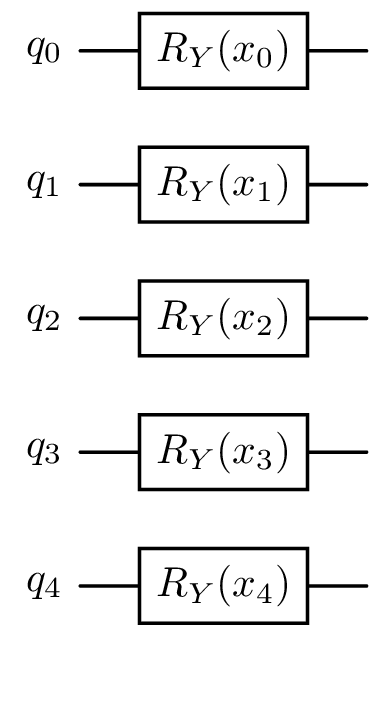
\includegraphics[width=\textwidth]{../images/encoders/quantikz/A1.png}
	%               \caption{}
	%               \label{fig:A1}
	%       \end{subfigure}%
%       \hfill
%       \begin{subfigure}{0.3\textwidth}
	%               \centering
	%               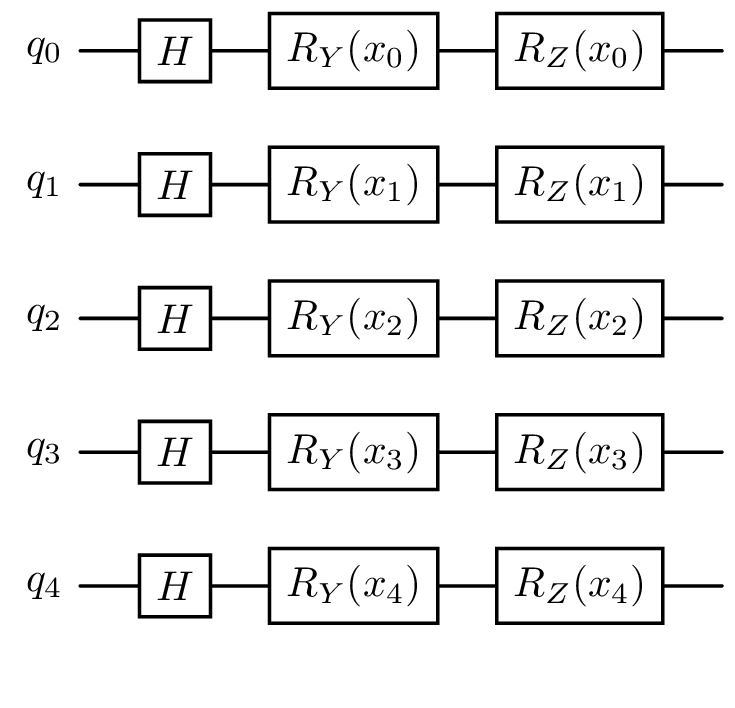
\includegraphics[width=\textwidth]{../images/encoders/quantikz/A2.png}
	%               \caption{}
	%               \label{fig:A2}
	%       \end{subfigure}%
%       \hfill
%       \begin{subfigure}{0.3\textwidth}
	%               \centering
	%               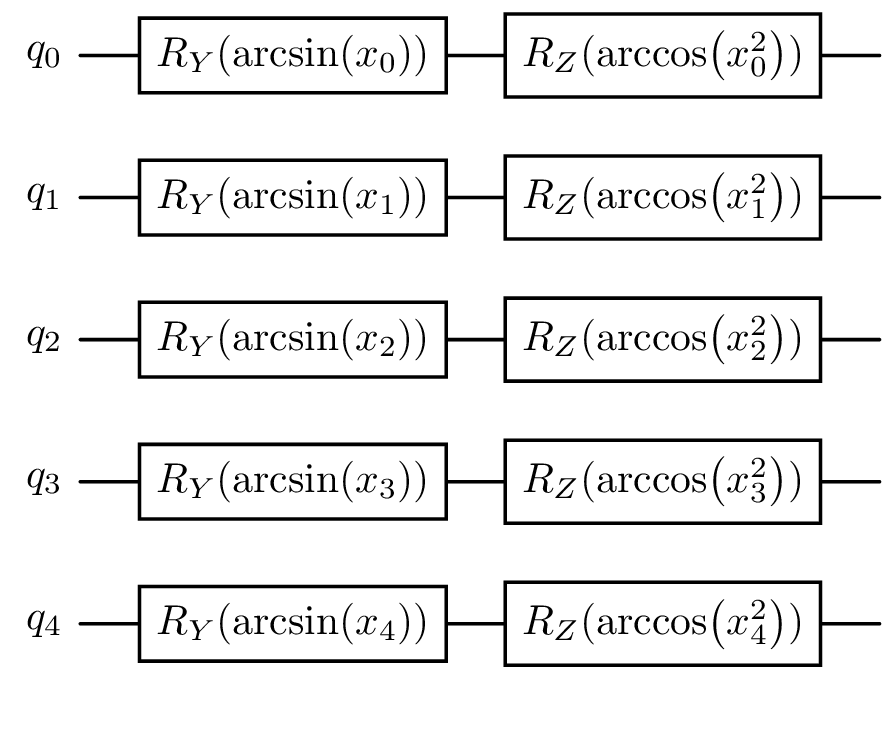
\includegraphics[width=1\textwidth]{../images/encoders/quantikz/M.png}
	%               \caption{}
	%               \label{fig:M}
	%       \end{subfigure}%
%       \hfill
%       \begin{subfigure}{1\textwidth}
	%               \centering
	%                   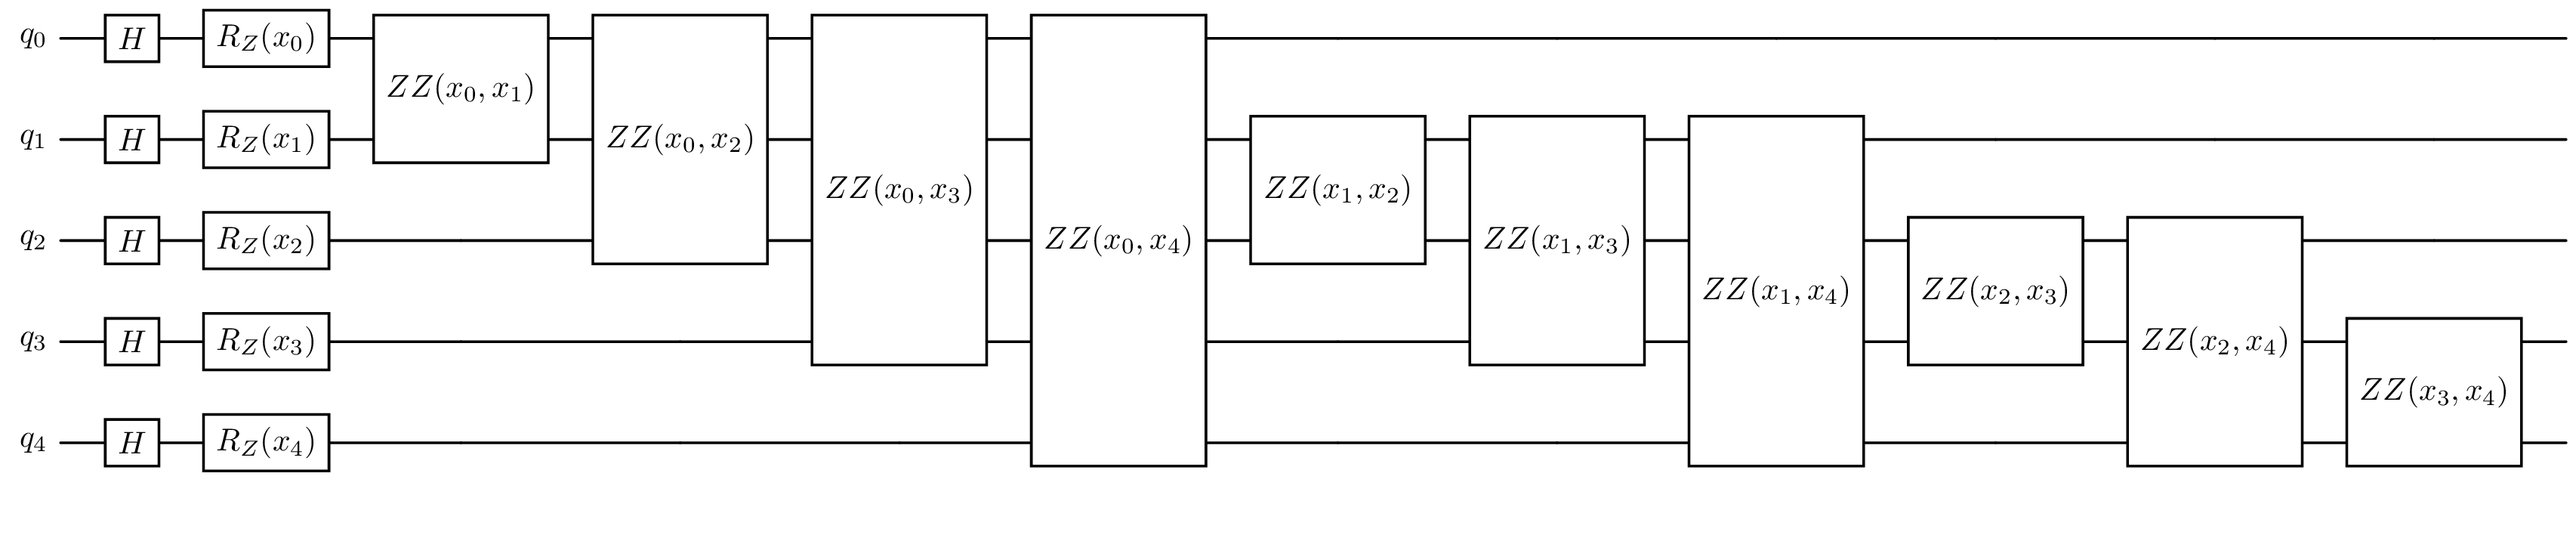
\includegraphics[width=\textwidth]{../images/encoders/quantikz/IQP.png}
	%               \caption{}
	%               \label{fig:IQP}
	%       \end{subfigure}%
%       \caption{(a) Single angle (A1) encoding, (b) double angle (A2) encoding, (c) Mitarai (M) encoding, and (d) Instantaneous Quantum Polynomial (IQP) encoding}
%       \label{fig:encoders}
%\end{figure}



  
\begin{figure}[H]
	\centering
	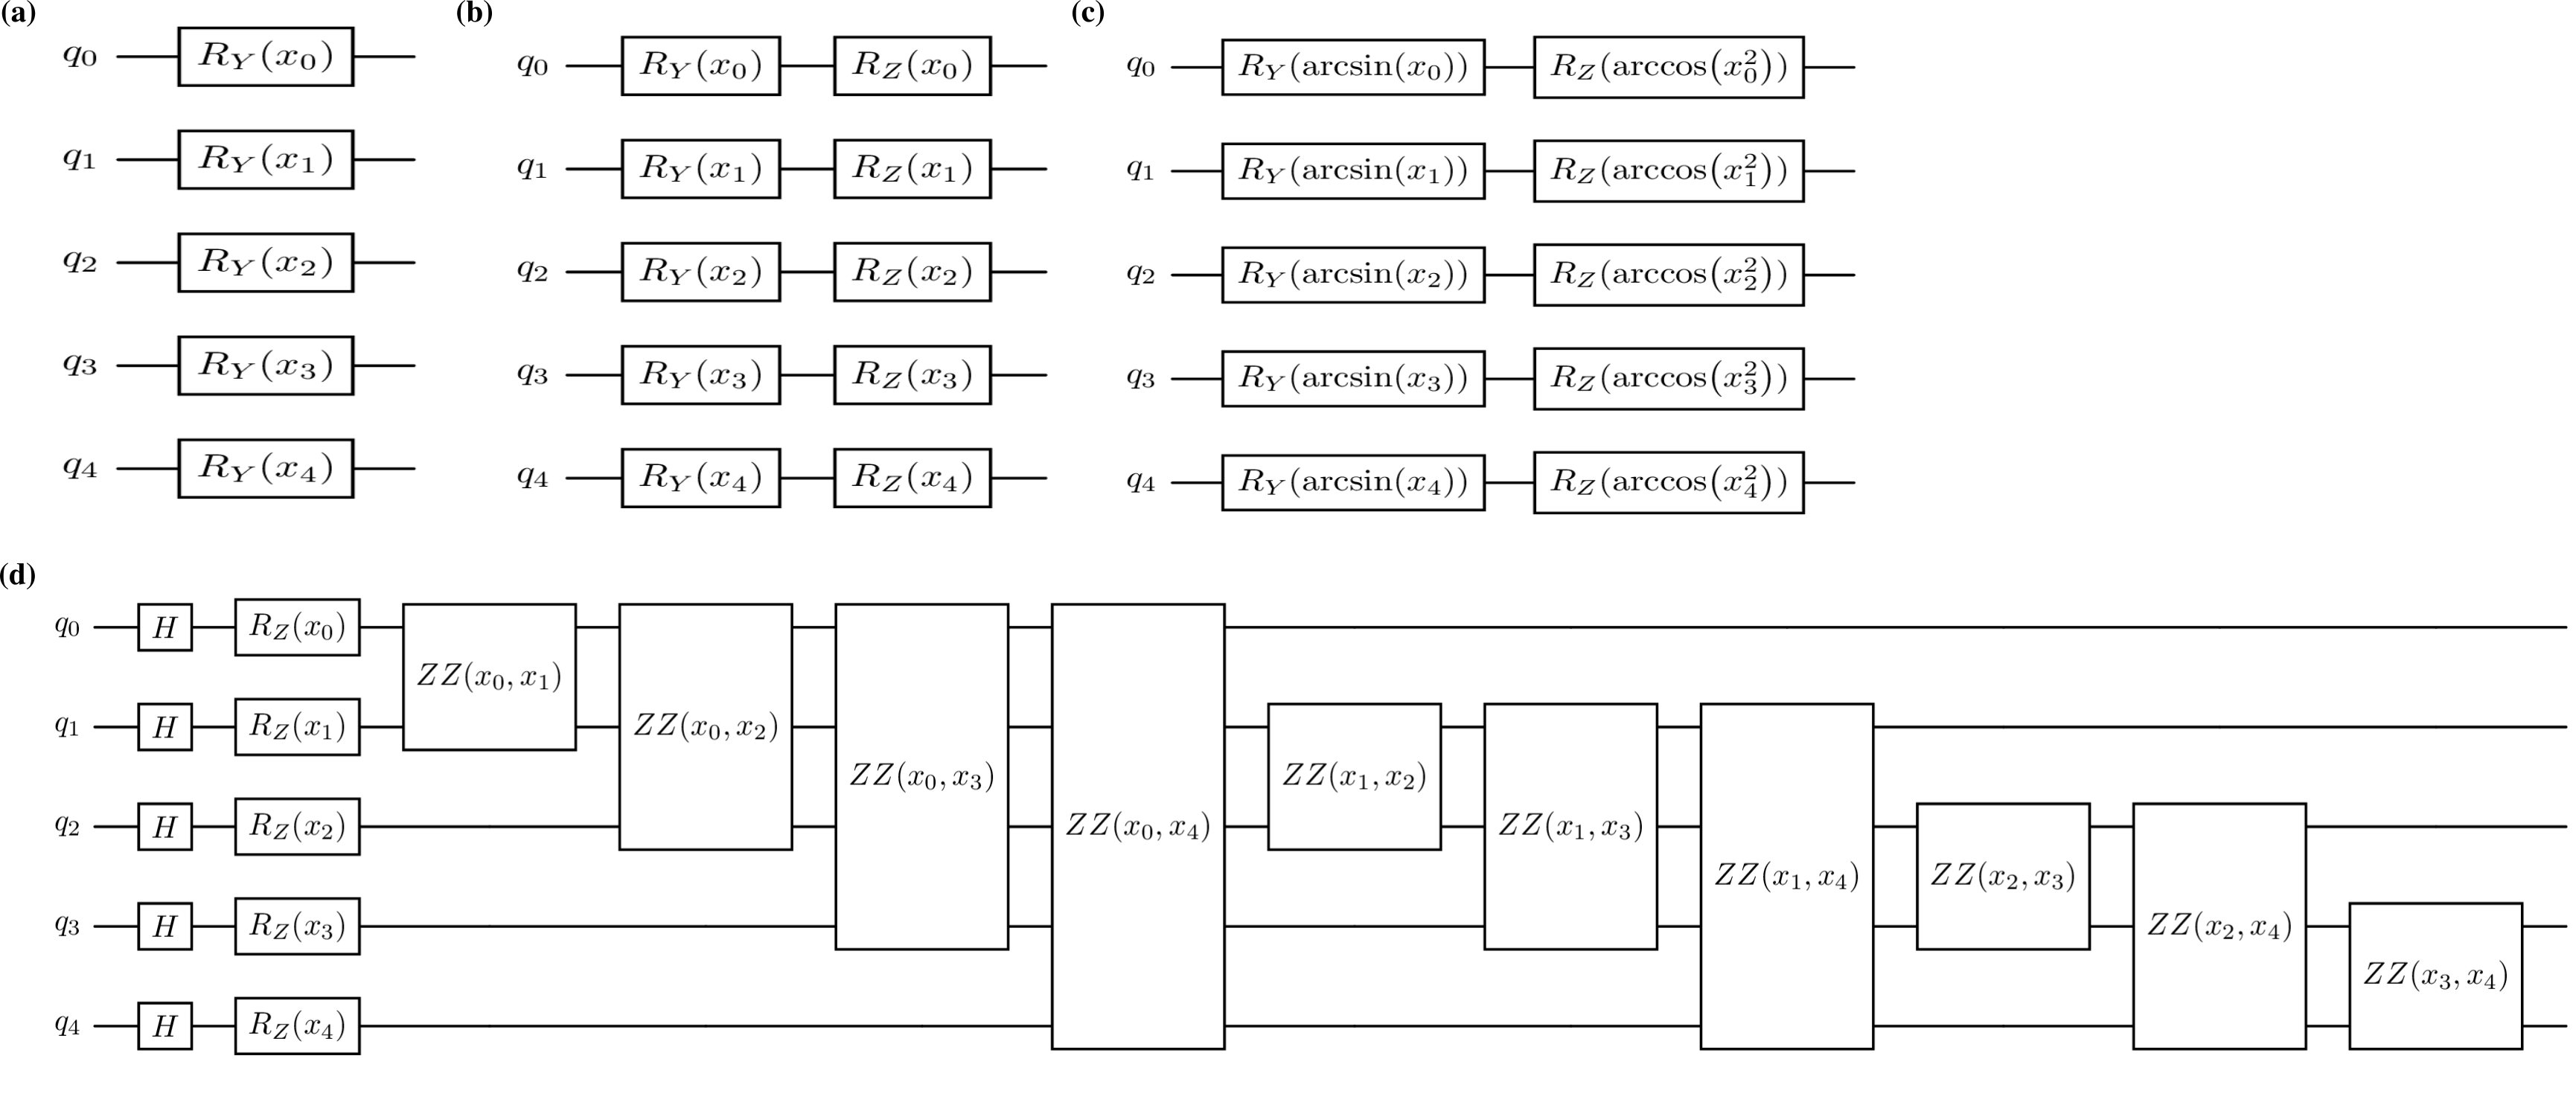
\includegraphics[width=\textwidth]{../images/encoders/quantikz/combined.png}
	\caption{(a) Single angle (A1) encoding, (b) double angle (A2) encoding, (c) Mitarai (M) encoding, and (d) Instantaneous Quantum Polynomial (IQP) encoding}
	\label{fig:encoders}
\end{figure}





  
When $l=2$, like in Ref. \citep{suzuki_predicting_2020} we choose entanglement gates, $E_{\text{ent}}^{1}$ and $E_{\text{ent}}^{2}$ to be equivalent, and the encoding layer takes the following form, $U_{\Phi(x)} =  E_{\text{ent}} U_{\phi_{2}(\mathbf{x})} E_{\text{ent}} U_{\phi_{1}(\mathbf{x})}$ .
We also exclude IQP encoding when $l=2$ due to the increased circuit depth, when compared to A1, A2, and M encoding.
Therefore, there are five unique combinations of $U_{\phi_{1}(\mathbf{x})}$ and $U_{\phi_{2}(\mathbf{x})}$ (M-M, A1-A1, A2-A2, M-A1, and M-A2) and two different entanglement layer options (CNOT and CZ) for a total of 10 encoding circuits. 
These circuits are denoted as $U_{\phi_{1}(\mathbf{x})}-U_{\phi_{2}(\mathbf{x})}-E_{\text{ent}}$, for example, two example encoding circuits are M--M--CNOT and M--A1--CNOT.
Table \ref{tab:encoders} shows all fourteen encoding circuits examined in this study.

\begin{table}[htbp]
	\centering
	\begin{tabular}{|c|c|c|c|}
		\hline
		\textbf{Name} & $U_{\phi_{1}(\mathbf{x})}$ & $U_{\phi_{2}(\mathbf{x})}$ & $E_{\text{ent}}$  \\
		\hline
		\hline
		A1 & $U_{\text{A1}}$ & --- & --- \\
		\hline
		A2 & $U_{\text{A2}}$ & --- & --- \\
		\hline		
		M & $U_{\text{M}}$ & --- & --- \\
		\hline
		IQP & $U_{\text{IQP}}$ & --- & --- \\
		\hline
		A1--A1--CNOT & $U_{\text{A1}}$ & $U_{\text{A1}}$ & $E_{\text{CNOT}}$ \\
		\hline
		 A2--A2--CNOT & $U_{\text{A2}}$ & $U_{\text{A2}}$ & $E_{\text{CNOT}}$ \\
		\hline
		M--M--CNOT & $U_{\text{M}}$ & $U_{\text{M}}$ & $E_{\text{CNOT}}$ \\
		\hline
		M--A1--CNOT & $U_{\text{M}}$ & $U_{\text{A1}}$ & $E_{\text{CNOT}}$ \\
		\hline		
		M--A2--CNOT & $U_{\text{M}}$ & $U_{\text{A2}}$ & $E_{\text{CNOT}}$ \\
		\hline				
		A1--A1--CZ & $U_{\text{A1}}$ & $U_{\text{A1}}$ & $E_{\text{CZ}}$ \\
		\hline
		A2--A2--CZ& $U_{\text{A2}}$ & $U_{\text{A2}}$ & $E_{\text{CZ}}$ \\
		\hline
		M--M--CZ & $U_{\text{M}}$ & $U_{\text{M}}$ & $E_{\text{CZ}}$ \\
		\hline
		M--A1--CZ & $U_{\text{M}}$ & $U_{\text{A1}}$ & $E_{\text{CZ}}$ \\
		\hline		
		M--A2--CZ & $U_{\text{M}}$ & $U_{\text{A2}}$ & $E_{\text{CZ}}$ \\
		\hline						
	\end{tabular}
	\caption{Add something smart}
	\label{tab:encoders}
\end{table}



Following the encoding layers,variational (or ansatz) layers are used to introduce trainable parameters into the quantum circuit.
We use a mixed notation from Refs. \citep{suzuki_predicting_2020} and \citep{sim_expressibility_2019}, since Ref. \citep{sim_expressibility_2019} contains all of the variational layers used within this work.
We relegate the discussion of the expressibility and entanglement examined in that work to Section \ref{section:results_and_discussion}.
A general variational layer can be denoted as,
\begin{equation}
	U(\bm{\theta}) = \prod_{v} U_{v}(\bm{\theta}_{v}), % E_{\text{ent}}^{v}
	\label{eq:general_variational}
\end{equation}
where $\bm{\theta}$ denotes the variational parameters and $v$ denotes the number of times that the layer is repeated within the circuit. 
As $v$ increases and the number of trainable parameters ($\bm{\theta}$) increase, the theoretical assumption is that the model expressibility should also increase.
In our study, we the number of variational layers as the number of ansatz layers (ALs).
%In our study, we choose $v \in \{1, 3, 5\}$ and refer to this as the number of ansatz layers (ALs).
We examine 12 different variational circuits, as shown in Fig. \ref{fig:ansatz}, which are denoted using the following labels: Modified-Pauli-CRZ (Fig. \ref{fig:ansatz}\textbf{(a)}) , Modified-Pauli-CRX (Fig. \ref{fig:ansatz}\textbf{(b)}), Efficient-CRZ (Fig. \ref{fig:ansatz}\textbf{(c)}), Efficient-CRX (Fig. \ref{fig:ansatz}\textbf{(d)}),, HWE-CNOT (Fig. \ref{fig:ansatz}\textbf{(e)}), HWE-CZ (Fig. \ref{fig:ansatz}\textbf{(f)}), ESU2 (Fig. \ref{fig:ansatz}\textbf{(g)}), Full-Pauli-CRZ (Fig. \ref{fig:ansatz}\textbf{(h)}), Full-Pauli-CRX (Fig. \ref{fig:ansatz}\textbf{(i)}), Hadamard (Fig. \ref{fig:ansatz}\textbf{(j)}), Full-CRZ (Fig. \ref{fig:ansatz}\textbf{(k)}), and Full-CRX (Fig. \ref{fig:ansatz}\textbf{(l)}),

\begin{figure}[H]
	\centering
	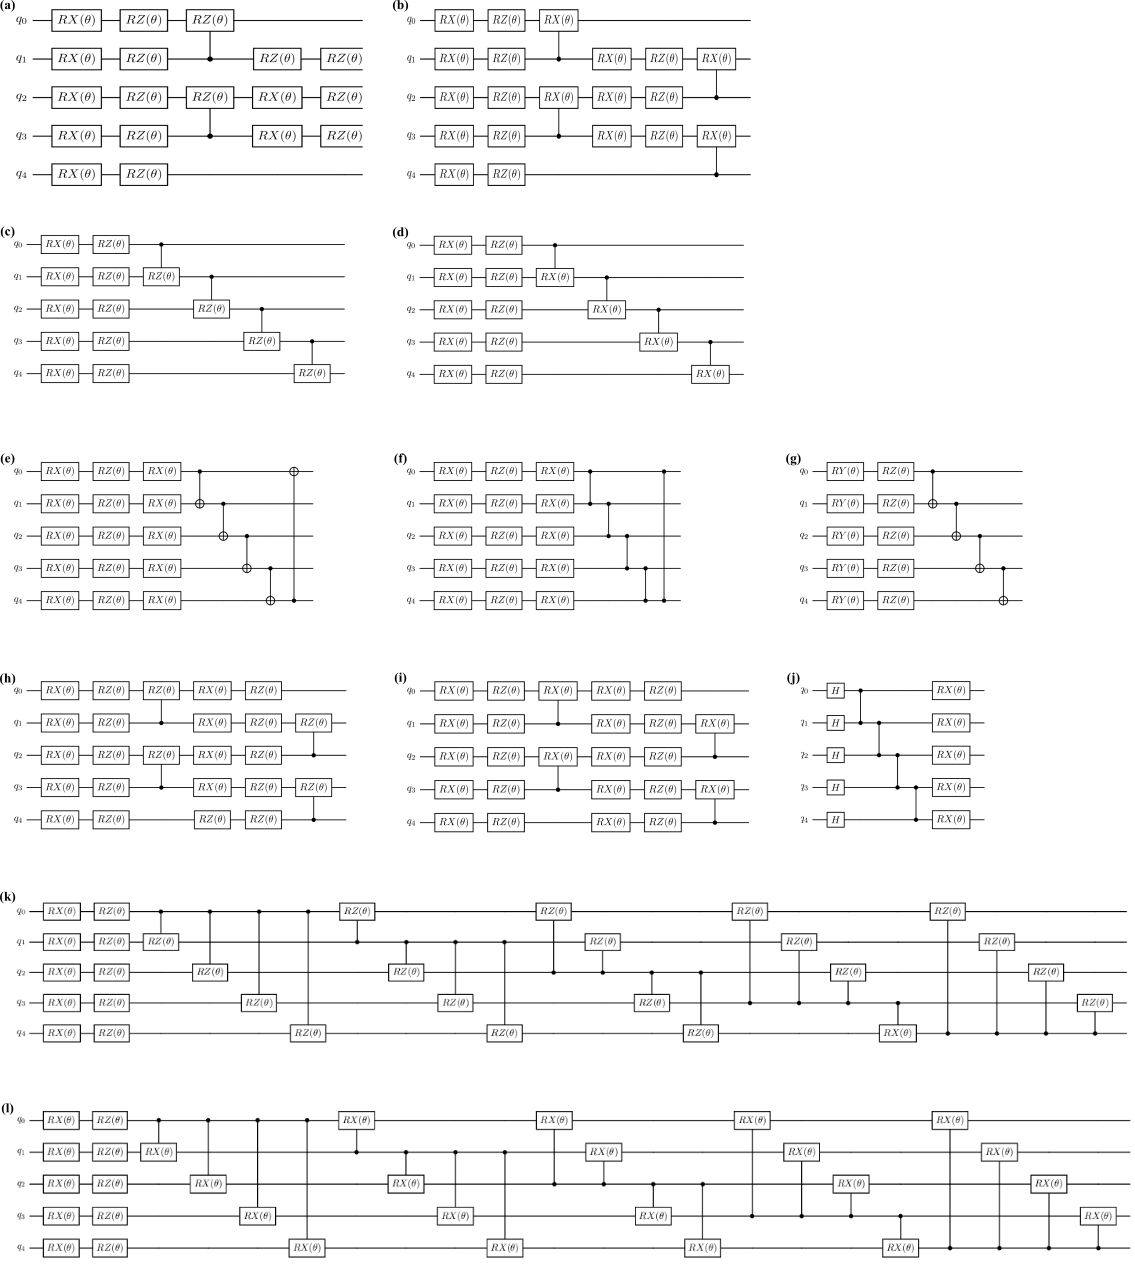
\includegraphics[width=\textwidth]{../images/ansatz/quantikz/combined.png}
	\caption{(a) Modified-Pauli-CRZ, (b) Modified-Pauli-CRX, (c) Efficient-CRZ, (d) Efficient-CRX, (e) HWE-CNOT, (f) HWE-CZ,  (g) ESU2, (h) Full-Pauli-CRZ, (i) Full-Pauli-CRX, (j) Hadamard, (k) Full-CRZ, and (l)Full-CRX}
	\label{fig:ansatz}
\end{figure}

Now that we have define the encoding (Eq. \ref{eq:general_encoding}) and variational (Eq. \ref{eq:general_variational}) circuits, we can then combine them to denote a general, complete circuit as,
\begin{equation}
	\ket{\Psi} = U(\bm{\theta}) U_{\Phi(\mathbf{x})}\ket{0}^{\otimes n} = \prod_{k}
	\left( \prod_{v} U_{v}(\bm{\theta}_{v}) \prod_{l} E_{\text{ent}}^{l} U_{\phi_{l}(\mathbf{x})} \right)  \ket{0}^{\otimes n},
\end{equation}
where we choose $k \in \{1, 3, 5\}$, which denotes the re-upload depth (RUD) of the circuit.
When a sufficient number of data re-uploading occur, it has been shown by P\'{e}rez-Salinas \textit{et al.} that data re-uploading is equivalent to the Universal Approximation Theorem for artificial neural networks.\cite{perez-salinas_data_2020}


Lastly, to recover the predicted target values, $\hat{y}_{i}$, from our quantum circuits, measurement of the quantum state, $\ket{\Psi}$, must be performed.
To perform this operation, we apply the Pauli Z operator on the first qubit denoted as,
\begin{equation}
	\hat{y}_{i} = \bra{\Psi}Z_{0}\ket{\Psi}_{i}.
	\label{eq:y_pred}
\end{equation}
The set of predicted target values, $\bm{\hat{y}} = (\hat{y}_{1}, \ldots, \hat{y}_{N}) \in \mathbb{R}^{N}$, where $N$ is the number of samples, is then passed to the loss function, $\mathcal{L}(\bm{y}, \bm{\hat y})$, where $y_{i}$ belongs to the set of true target values $\bm{y} = (y_{1}, \ldots, y_{N}) \in \mathbb{R}^{N}$.
In practice, $\mathcal{L}$ can be any loss function but we choose to use the mean square error loss function denoted as,
\begin{equation}
	\mathcal{L}(\bm{y}, \bm{\hat y}) = \frac{1}{N} \sum_{i=1}^{N} (y_{i} - \hat{y}_{i})^{2}.
	\label{eq:isthisloss}
\end{equation}


\subsection{Implementation}
\begin{figure}[H]
	\centering
	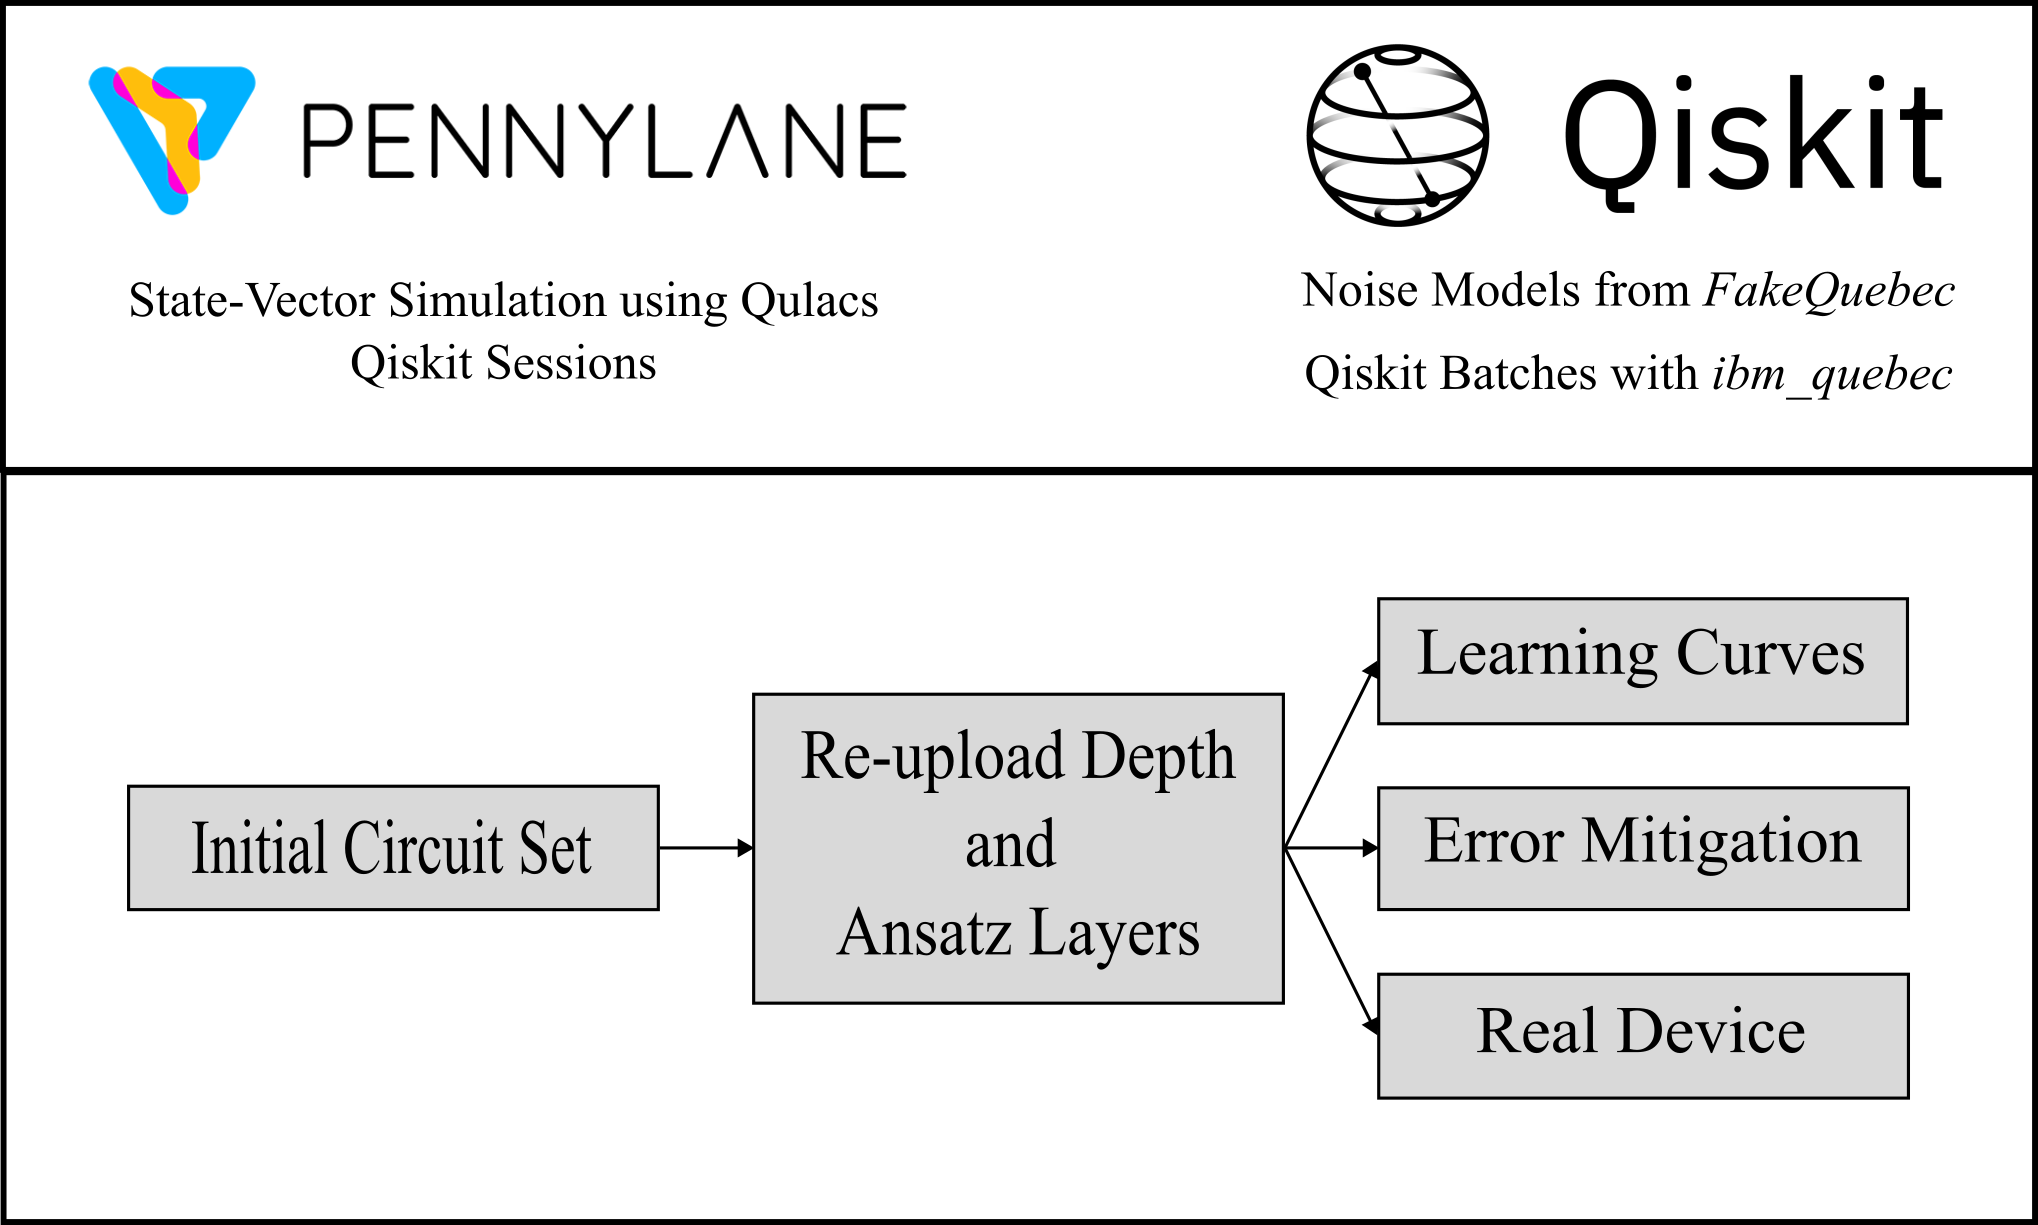
\includegraphics[width=\linewidth]{../images/manuscript_figures/overview.png}
	\caption{Make this figure highlight the modularity of \textit{qregress}}
	\label{fig:overview_project}
\end{figure}

We introduce \textit{qregress}, a modular Python package for regression-based PQCs.

We perform all simulation calculations using PennyLane\cite{bergholm_pennylane_2022}, either using Qulacs\cite{suzuki_qulacs_2021} for state vector calcualtions, while noisy calculations were performed using \textit{qiskit-aer} with the \textit{FakeQuebec} backend as implemented in the PennyLane-Qiskit plugin.\cite{javadi-abhari_quantum_2024}
We perform calculations in the \textit{ibm\_quebec} device using circuits implemented using Qiskit\cite{javadi-abhari_quantum_2024}, due to issues we initially faced with running experiments on the real device using the PennyLane-Qiskit plugin.
For the experiments using PennyLane,  we utilize the Simultaneous Perturbation Stochastic Approximation method (SPSA) as implemented in PennyLane, while for the experiments run on \textit{ibm\_quebec} utilizes the Constrained Optimization By Linear Approximation (COBYLA) optimizer as implemented ing SciPy\cite{virtanen_scipy_2020}.
Each optimizer was chosen based on the performance for the given task.
All features ($\mathbf{x}$) and target values ($\mathbf{y}$) were scaled using the MinMaxScaler in Scikit-learn\cite{pedregosa_scikit-learn_2011}, such that all featues and target values are $\mathbb{R}\in [ -1,1 ]$.
For the simulations using \textit{FakeQuebec} and experiments on \textit{ibm\_quebec} we utilize Twirled Readout Error eXtinction (TREX) error mitigation.



Used QisKit for real and fake back end using Qiskit Batches

optimization levels
none (0) 

``No optimization: typically used for hardware characterization
Basic translation and Layout/Routing: TrivialLayout, where it selects the same physical qubit numbers as virtual and inserts SWAPs to make it work (using StochasticSwap)''


light (1)
``Light optimization: Layout/Routing: Layout is first attempted with TrivialLayout. If additional SWAPs are required, a layout with a minimum number of SWAPs is found by using SabreSWAP, then it uses VF2LayoutPostLayout to try to select the best qubits in the graph, InverseCancellation, 1Q gate optimization''

medium (2)
``Medium optimization: Layout/Routing: Optimization level 1 (without trivial) + heuristic optimized with greater search depth and trials of optimization function. Because TrivialLayout is not used, there is no attempt to use the same physical and virtual qubit numbers. CommutativeCancellation''

high (3)
``High Optimization:
Optimization level 2 + heuristic optimized on layout/routing further with greater effort/trials
Resynthesis of two-qubit blocks using Cartan's KAK Decomposition.
Unitarity-breaking passes:
OptimizeSwapBeforeMeasure: Moves the measurements around to avoid SWAPs
RemoveDiagonalGatesBeforeMeasure: Removes gates before measurements that would not effect the measurements''


resilience levels (error mitigation)
none (0) 
level 1 readout error mitigation and measurement twirling using Twirled Readout Error eXtinction (TREX) \cite{van_den_berg_model-free_2022}
level 2 level 1 + gate twirling and zero noise extrapolation (ZNE)\cite{kandala_error_2019,li_efficient_2017,temme_error_2017}

Function fitting 5: all ran with 1000 iterations
Function fitting 16: all ran with 1000 iterations
BSE 5: all ran with 1000 iterations
BSE 16: all ran with 1000 iterations
DDCC

\subsection{Datasets}\label{subsection:datasets}
In this study, we explore two datasets: a dataset of bond separation energies (BSE) of molecules (Figs. \ref{fig:bondtypes} and \ref{fig:BSEdistr}), where the feature set encodes structural information of each molecule;
and a dataset consisting of electronic structure features to predict wave functions using the data-driven coupled-cluster scheme of Townsend and Vogiatzis (Fig. \ref{fig:waterddccdistribution}).\cite{townsend_data-driven_2019}
We utilize the BSE49 and DDCC databases for two different reasons: the BSE49 database consists of a hard chemical property to predict using few features, while the DDCC dataset can be predicted easily using few features classically but is data intensive in the number of samples per molecule.

\begin{figure}[H]
	\centering
	\begin{subfigure}[b]{0.65\textwidth}
		\centering
		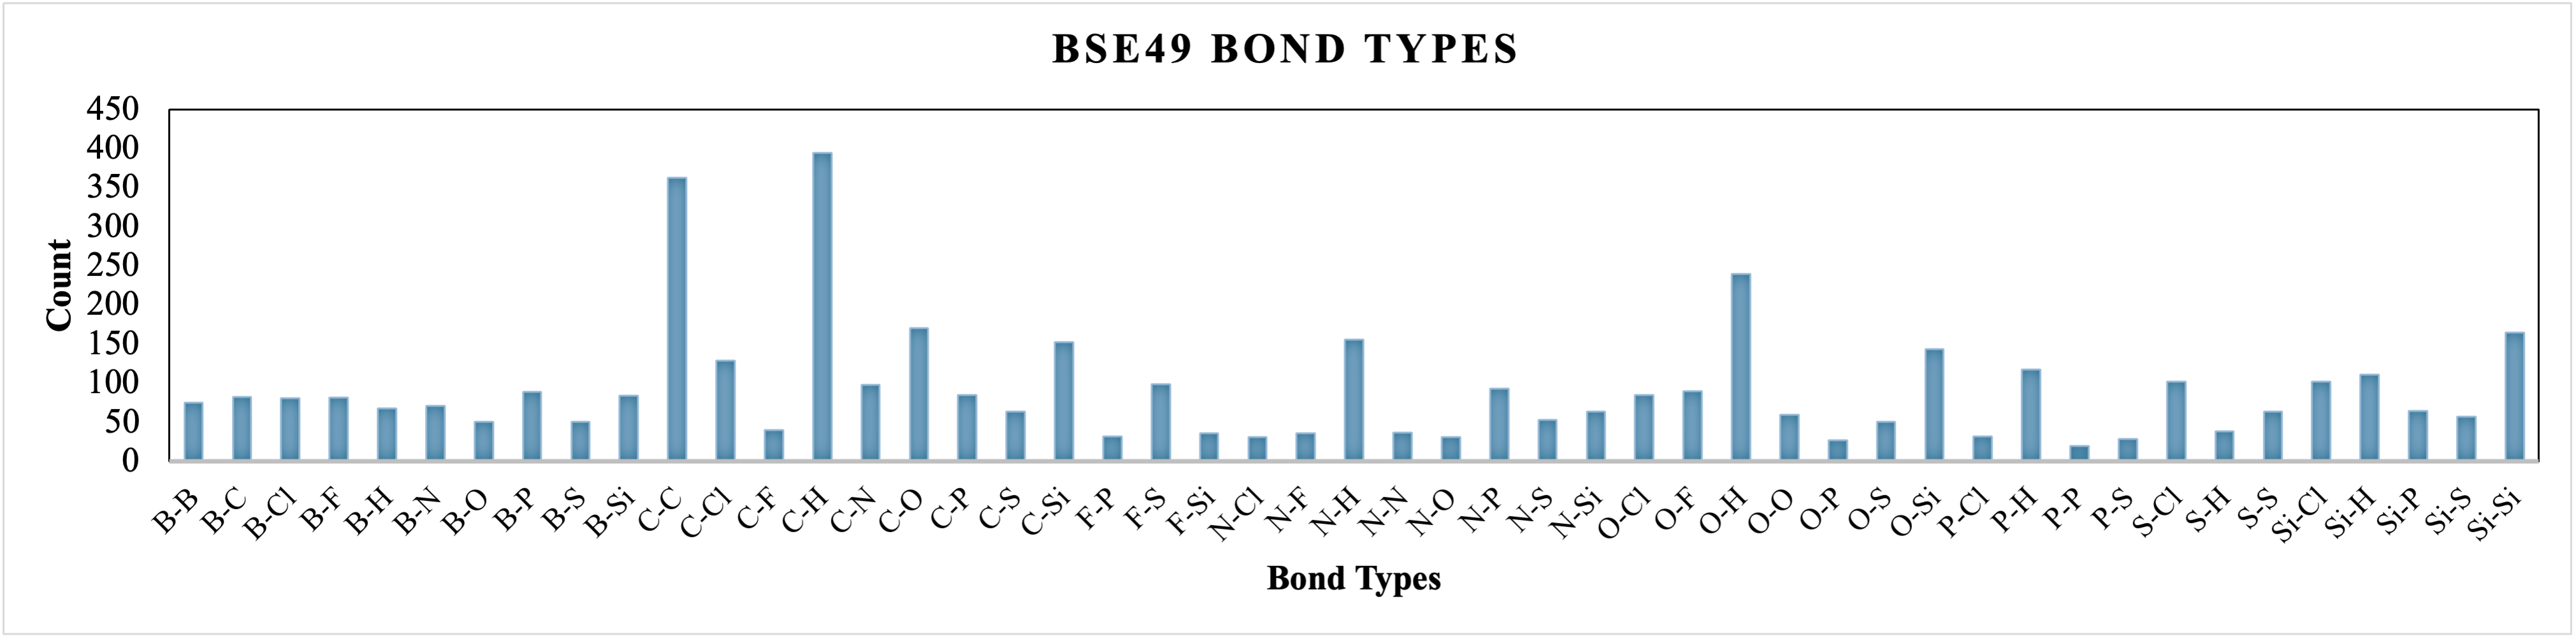
\includegraphics[width=\textwidth]{../images/BSE/bondtypes.png}
		\caption{}
		\label{fig:bondtypes}
	\end{subfigure}
	\hfill
	\begin{subfigure}[b]{0.3\textwidth}
		\centering
		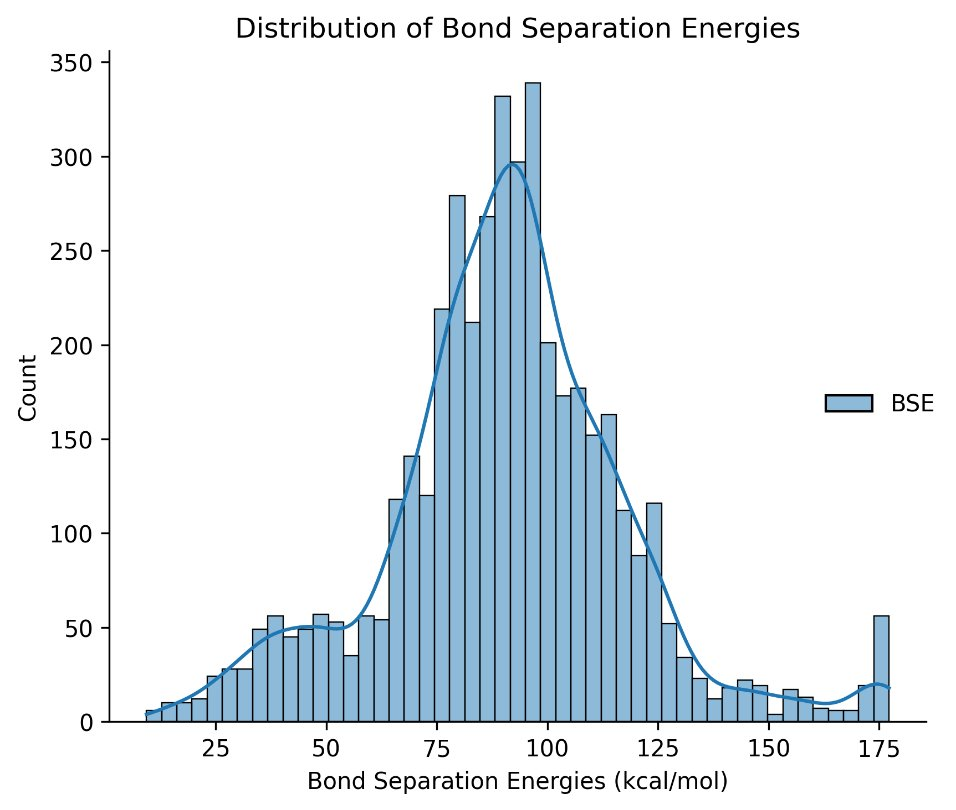
\includegraphics[width=\textwidth]{../images/BSE/BSE.jpg}
		\caption{}
		\label{fig:BSEdistr}
	\end{subfigure}
	\hfill
	\begin{subfigure}[b]{0.3\textwidth}
		\centering
		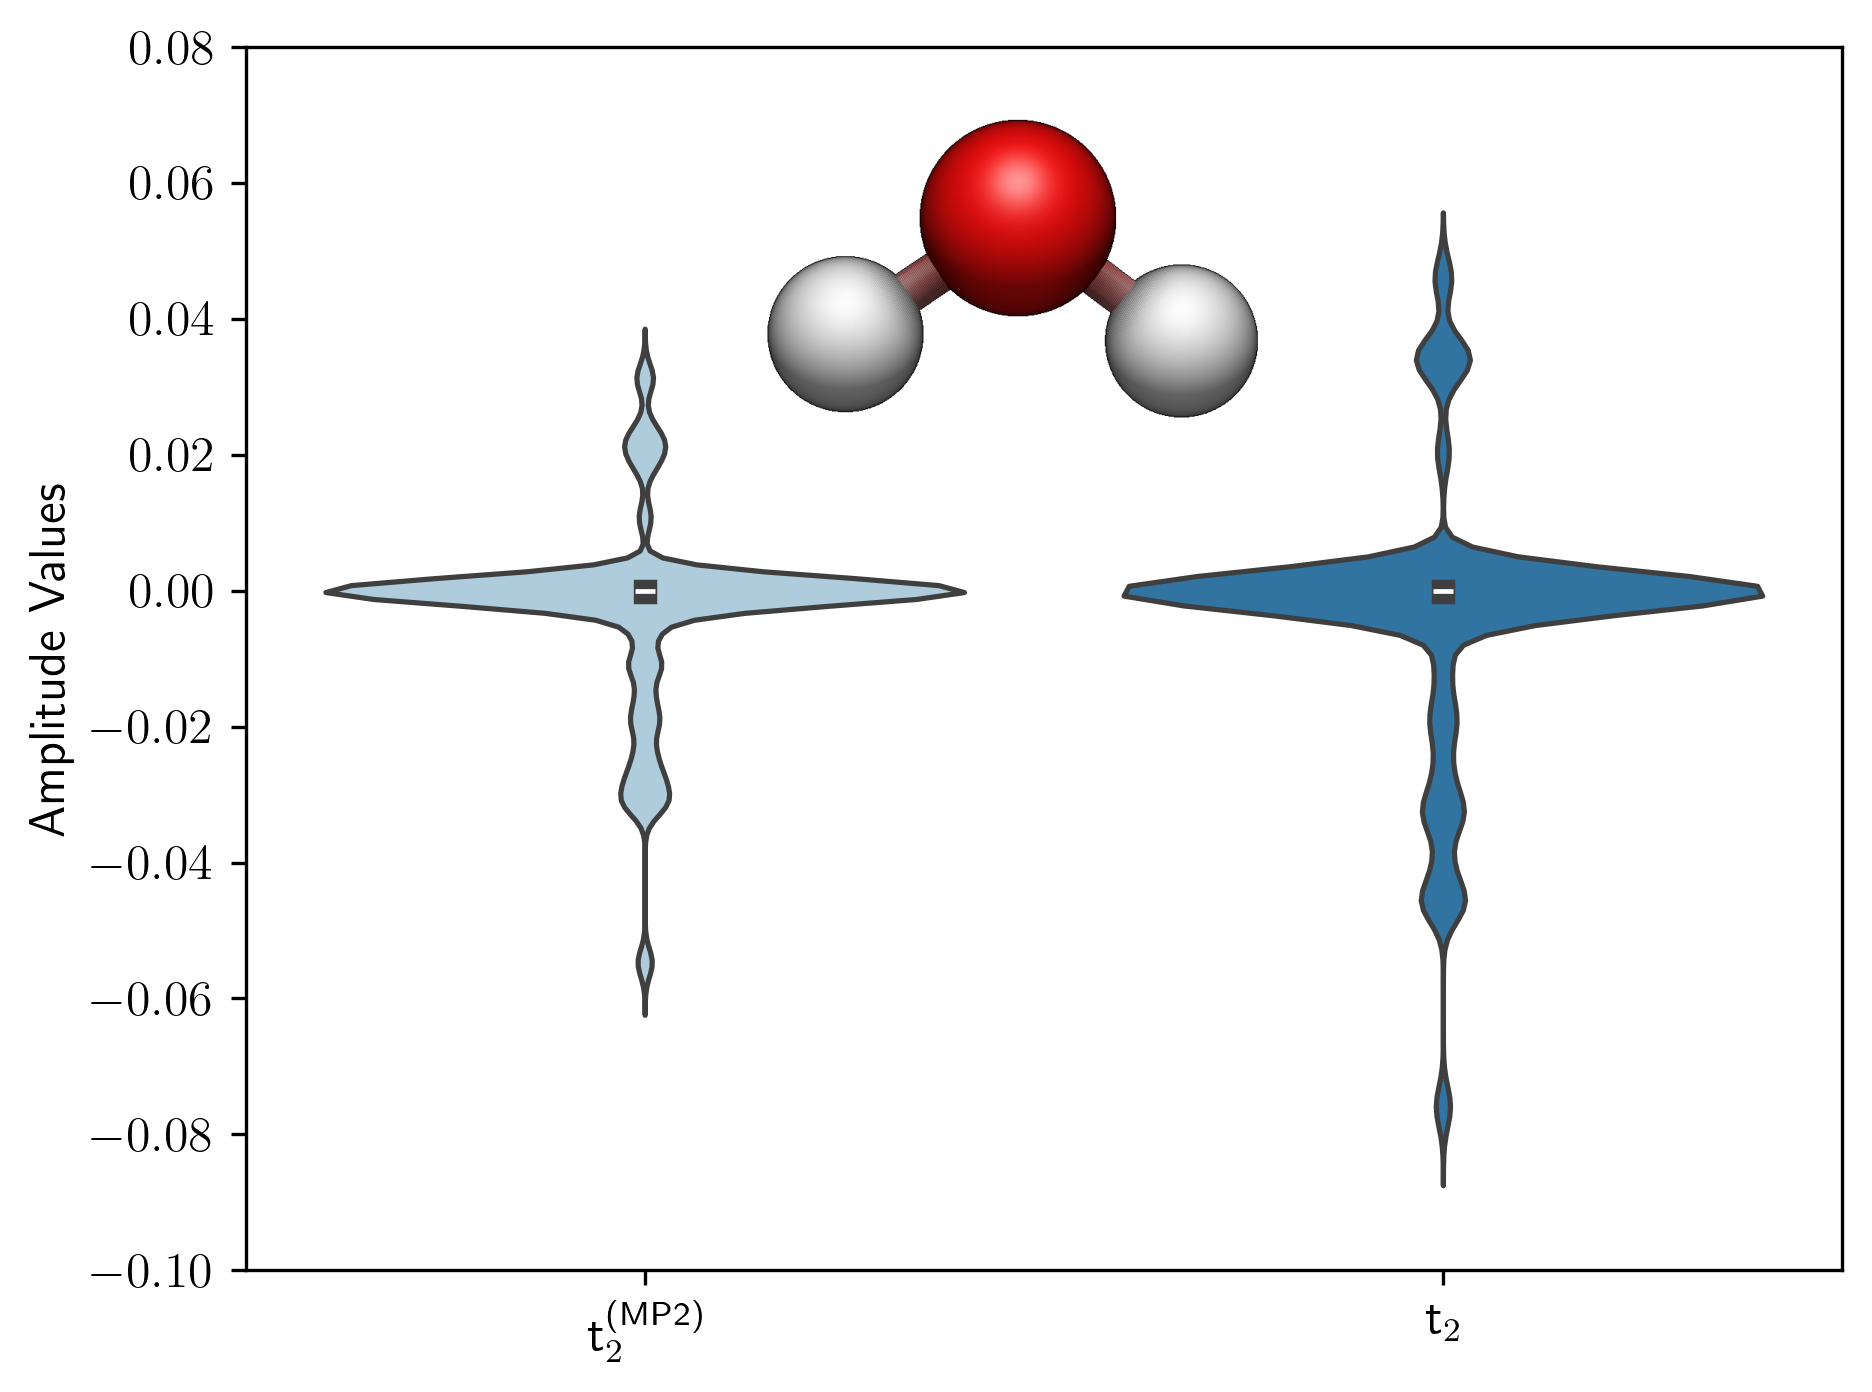
\includegraphics[width=\textwidth]{../images/manuscript_figures/waterddccdistribution.png}
		\caption{}
		\label{fig:waterddccdistribution}
	\end{subfigure}	
	\caption{Examples of the datasets explored in this study. For the BSE49 dataset the distributions of the (d) bond types and the (e) bond separation energies in kcal/mol. For the DDCC dataset distributions of the initial MP2 $t_{2}$-amplitudes and the optimized CCSD $t_{2}$-amplitudes are shown in (f).}
	\label{fig:bse_data}
\end{figure}


BSE49
``This work addresses the aforementioned gap in the literature by constructing a large dataset (4502 datapoints) of computationally predicted BSEs of 49 unique bond types, all of which are determined with a high-level composite theoretical procedure denoted as (RO)CBS-QB3. This approach ensures uniform, high-quality reference data and eliminates the need to collect and verify data gathered from various sources, which may differ substantially in their accuracy. The (RO)CBS-QB3 method is known to produce BDEs of high accuracy. Therefore, it is suitable for developing a database of BSEs that can be used to test and parametrize low-cost computational methods. One particular target application of our dataset is for the training of cost-effective computational approaches like atom-centered potentials (ACPs) or machine learning potentials.''
(RO)CBS-QB3\cite{wood_restricted-open-shell_2006,montgomery_complete_1999,montgomery_complete_2000}  

```The structures obtained from the workflow described above were then used for the final step of reference data calculation, using the composite (RO)CBS-QB331,32,33 method. The restricted-open-shell61 CBS-QB3 or ROCBS-QB3 was employed for the open-shell radical fragments, while restricted closed-shell calculations were performed for the closed-shell parent molecules with CBS-QB3. The composite (RO)CBS-QB3 method approximates energies at the complete-basis-set CCSD(T) level, using a series of computationally lower-cost methods including: (i) geometry optimization followed by vibration frequency calculation using the unrestricted-open-shell62 B3LYP/6-311G(2d,d,p) method46,47,48,49,50,51,63, (ii) ROMP2/6-311+G(3d2f,2df,2p) level63,64,65 energy extrapolated to the complete-basis-set limit, (iii) energy calculation at ROMP4(SDQ)/6-31+G(d(f),p) level63,64,66, and (iv) energy calculation at ROCCSD(T)/6-31+G† level63,64,67 (where 6-31+G† is a modified 6-31+G(d) basis set). Note that the final (RO)CBS-QB3 energy includes additional empirical correction terms described in Reference33. Structures were screened to remove any system for which the imaginary frequencies were obtained. The (RO)CBS-QB3 energies for the structures associated with a particular bond breaking reaction were used to obtain the bond separation energies for the dataset.'''



Following model calibration using the function fitting dataset, we explore the appliciblity of PQCs for complex chemically relevant machine learning tasks.
The first chemically motivated dataset we explore is the BSE49 dataset, which contains the bond seperation energies (BSE)  for the homolytic bond cleavage of covalently bonded molecules, such as \ce{A-B -> A^{.} + B^{.}}.\cite{prasad_bse49_2021}
This dataset consists of 4394 datapoints, 1951 of which are existing and 2443 are hypthoetical structures, with 49 unique A-B single bond types.
In practice, we used 2436 of the hypothetical structures due to issues with valency exceptions when converting to RDKit mol objects which were later used for generating our features for the machine learning models.
An important aspect of machine learning in chemistry is the choice of molecular representation, or how the molecule is represented in the machine learning models.\cite{jones_molecular_2023}
Using RDKit\cite{noauthor_rdkit_nodate} we examined three commonly applied graph-based molecular preresentations, Molecular ACCess Systems (MACCS)\cite{durant_reoptimization_2002}, Morgan or extended-connectivity fingerprints \cite{morgan_generation_1965,rogers_extended-connectivity_2010}, and RDKit fingerprints.
All three of these methods are use traversals of the molecular graphs to encode various structural details into bit vectors.
Lastly, we explore both topology- and physics-based molecular representations, both of which encode the three-dimensional structure of molecules in various, unique ways.
Persistent images (PIs) are a topology-based fingerprint that uses persistence homology to encode topological information of three-dimensional molecular structures into fixed dimension images.\cite{adams_persistence_2017,townsend_representation_2020,schiff_augmenting_2022} 
We use the implementation from Townsend \textit{et al.}\cite{townsend_representation_2020}, which uses the Ripser Python package to generate PIs.\cite{tralie_ripserpy_2018}
Lastly, we explre two physics-based representations, Coulomb matrices (CMs) \cite{rupp_fast_2012} and smooth overlap of atomic positions (SOAPs), that were generated using DScribe.\cite{de_comparing_2016}
Due to the computational cost of computing the regularized entropy match (REMatch) kernel  with the SOAPs representation, we excluded this representation in the overall discussion.
We  also tested two different methods for representing the components of the bond separation chemical reaction, one where the feature vectors for the products are subtracted from the reactants, denoted by \textit{sub}, similar to the method used in Ref. \cite{garcia-andrade_barrier_2023}, and one that is composed of the reactant molecular only, denoted as \textit{AB}.


Since we are analyzing a diverse set of PQCs, we also examine a diverse set of classic regression models, with varying capabilities, such as ridge, lasso, elastic net, \textit{k}-nearest-neighbors, random forest, gradient boosting, support vector, kernel ridge, and gaussian process regression as implemented in sckit-learn.\cite{pedregosa_scikit-learn_2011}
Based on our results shown in Fig. \ref{fig:classical_molrepfig} we found that Morgan fingerprints
We found that the best molecular representation across all models test, as shown in Fig. \ref{fig:classical_molrepfig}, was Morgan fingerprints using the \textit{sub} formulation.
 
\begin{figure}[H]
	\centering	
	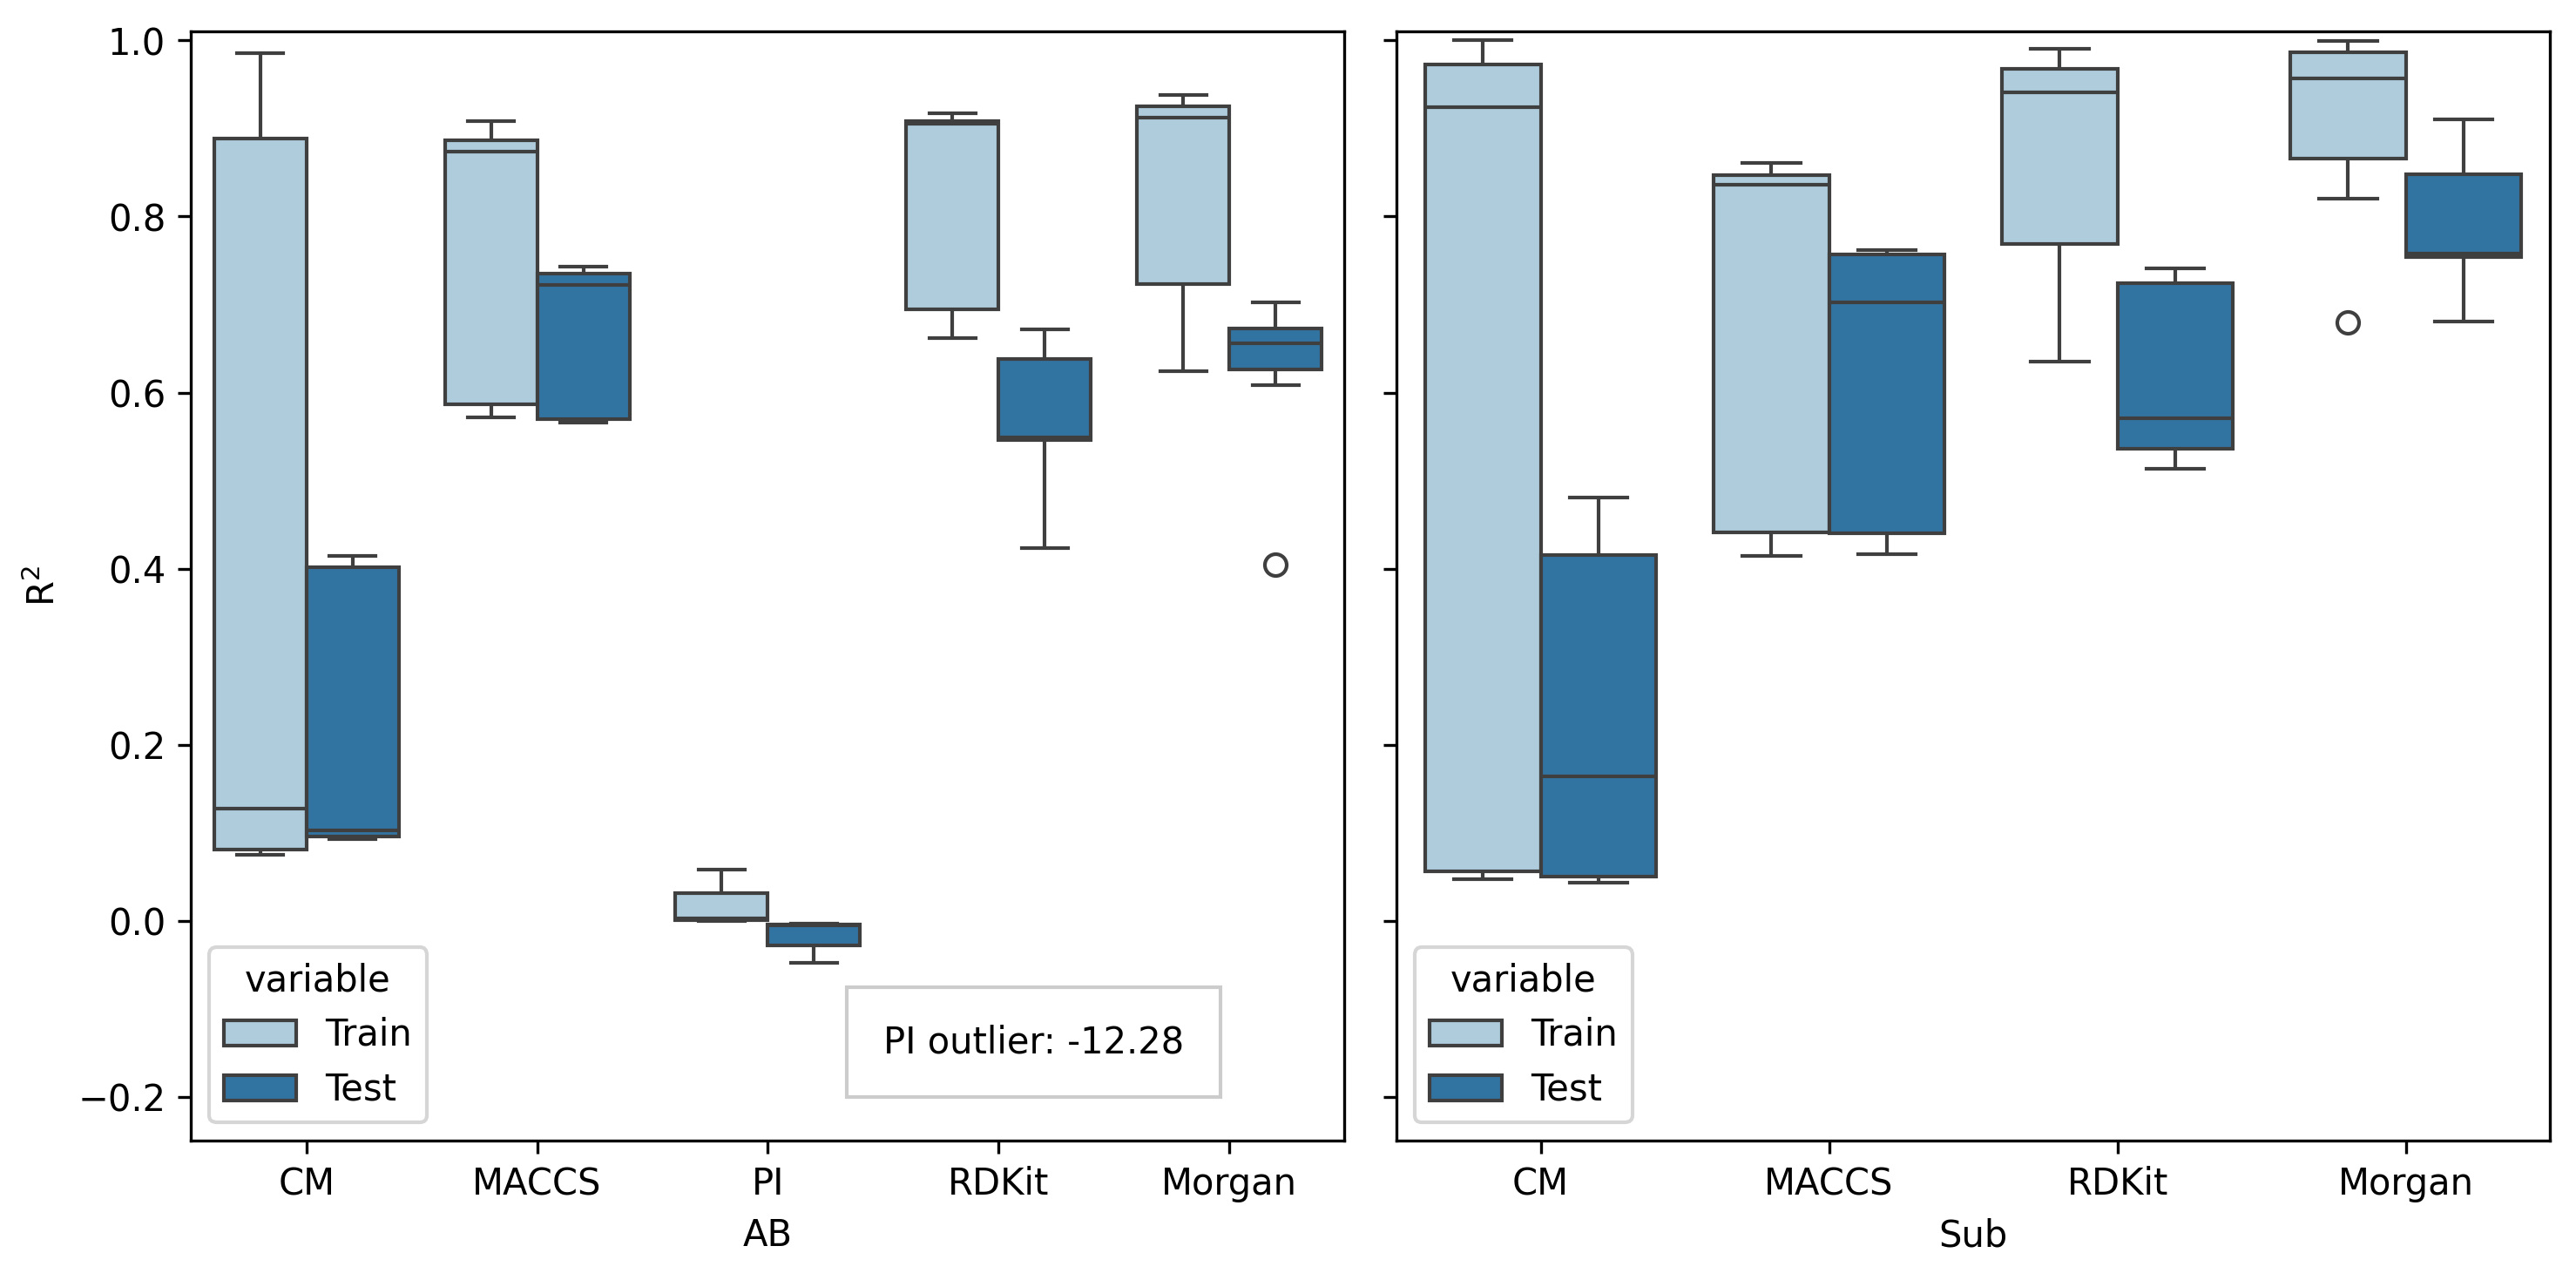
\includegraphics[width=\linewidth]{../images/BSE/classical/classical_molrepfig.png}
	\caption{Coulomb matrices (CMs), Molecular ACCess Systems (MACCS), persistence images (PIs), RDKit and Morgan fingerprints. Performance of a diverse set of molecular representations R$^{2}$}
	\label{fig:classical_molrepfig}
\end{figure}


An additional challenge of applying classical molecular representations for quantum machine learning models is mapping the classical features, often containing hundreds or thousands of features per sample, to the number of qubits used on the quantum device.
Initially, the Morgan fingerpints have 2048 features per sample, that need to be reduced down to 5 or 16 qubits.
We choose 5 and 16 qubits for two reasons, the first is that these were the standard number of qubits on IBM quantum devices when we started the project and the second is that reducing the number of features reduces the depth of the circuits.
To reduce the feature set from 2048 to 5 or 16 features, we explore two different methods, SHapley Additive ExPlanation analysis (SHAP)\cite{lundberg_unified_2017} and principal component analysis (PCA), as implemented in scikit-learn.\cite{pedregosa_scikit-learn_2011}
Figs. \ref{fig:BSE_classical_features_R2} and \ref{fig:BSE_bse_classical_features_MAE} show the results for the reductions using SHAP and PCA for the training and test set of using 5 and 16 features.
The initial model using 2048 features has a train and test mean absolute error (MAE) of 1.91 and 4.98 kcal/mol, with train and test R$^{2}$s of 0.99 and 0.91, respectively.
When using SHAP to reduce the feature set size to 5 features, we see that the training set has an MAE of 16.08 kcal/mol and an R$^{2}$ of 0.39, while for the test set has an MAE of 15.86 kcal/mol and an R$^{2}$ of 0.42.
When the number of features is reduced to 16 features using SHAP, we see slight improvements with train and test MAEs of 10.48 and 11.08 kcal/mol with R$^{2}$s of 0.69 and 0.68, respectively.
Using PCA, we see an improvement in accuracy for both 5 and 16 features, where the training sets have MAEs of 4.09 and 3.23 kcal/mol and the test sets have MAEs of 10.17 and 8.40 kcal/mol, respectively.
The R$^{2}$s for PCA with 5 and 16 features also shows improvement over the reductions using SHAP, with R$^{2}$s of 0.95 and 0.69 for the training and test set, respectively, using 5 features and 0.97 and 0.78 for the training and test set, respectively, using 16 features.
Due to the increased performance, despite exhibiting overfitting, we choose to use Morgan fingerprints reduced using PCA for our QML models.



\begin{figure}[H]
	\centering	
	\begin{subfigure}[b]{0.49\textwidth}
		\centering
		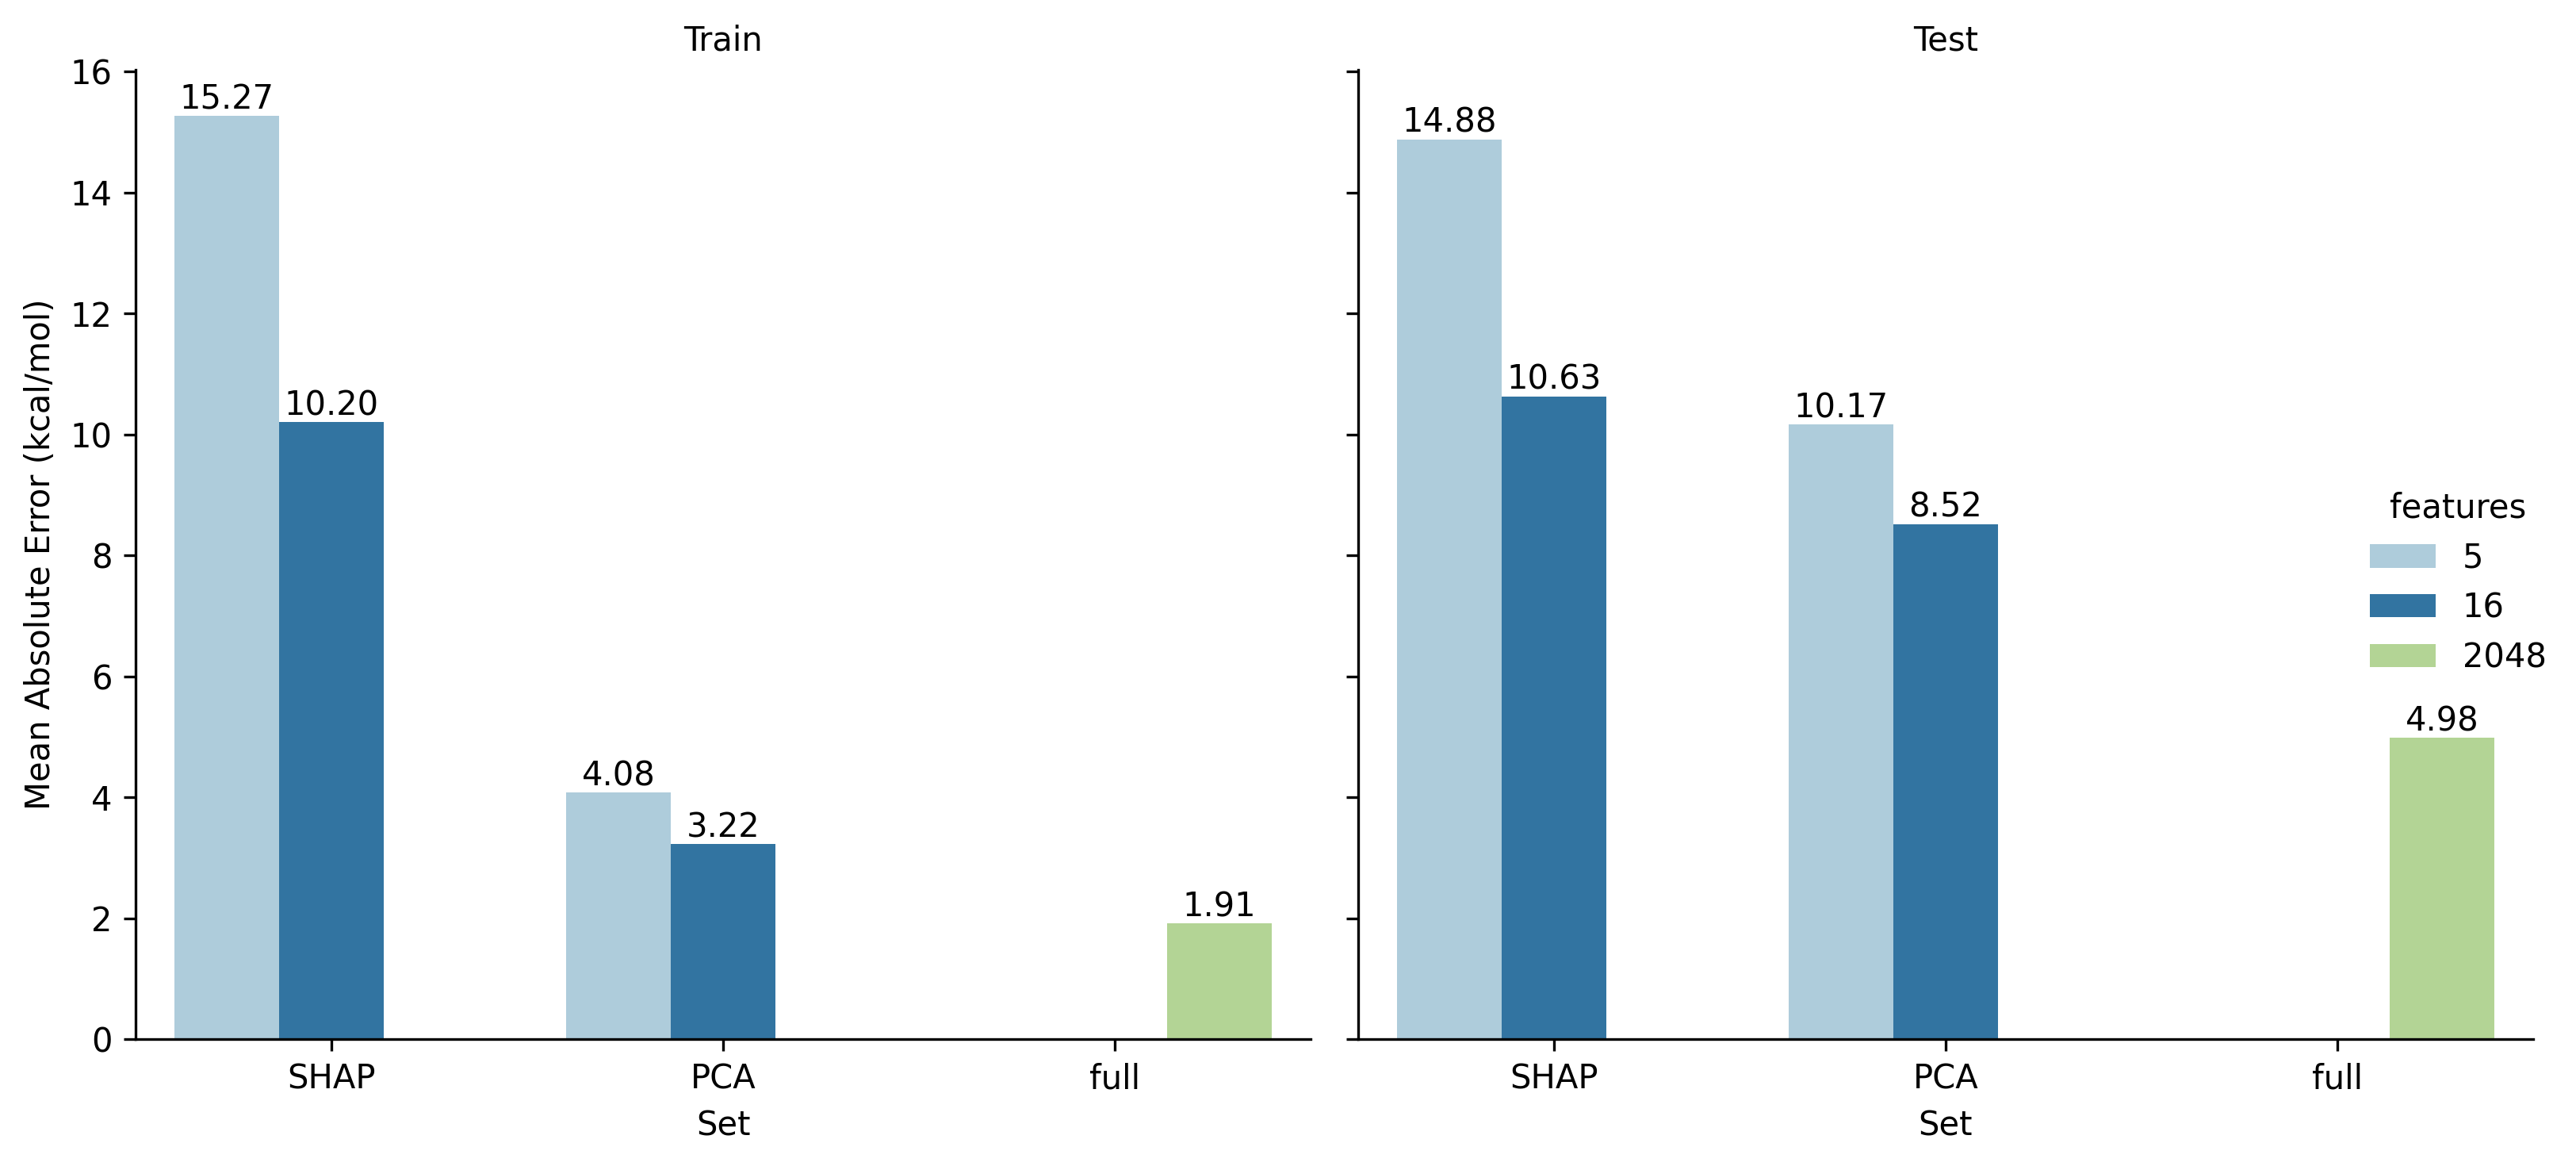
\includegraphics[width=\textwidth]{../images/BSE/classical_features_MAE.png}
		\caption{}
		\label{fig:BSE_bse_classical_features_MAE}
	\end{subfigure}
	\hfill		
	\begin{subfigure}[b]{0.49\textwidth}
		\centering
		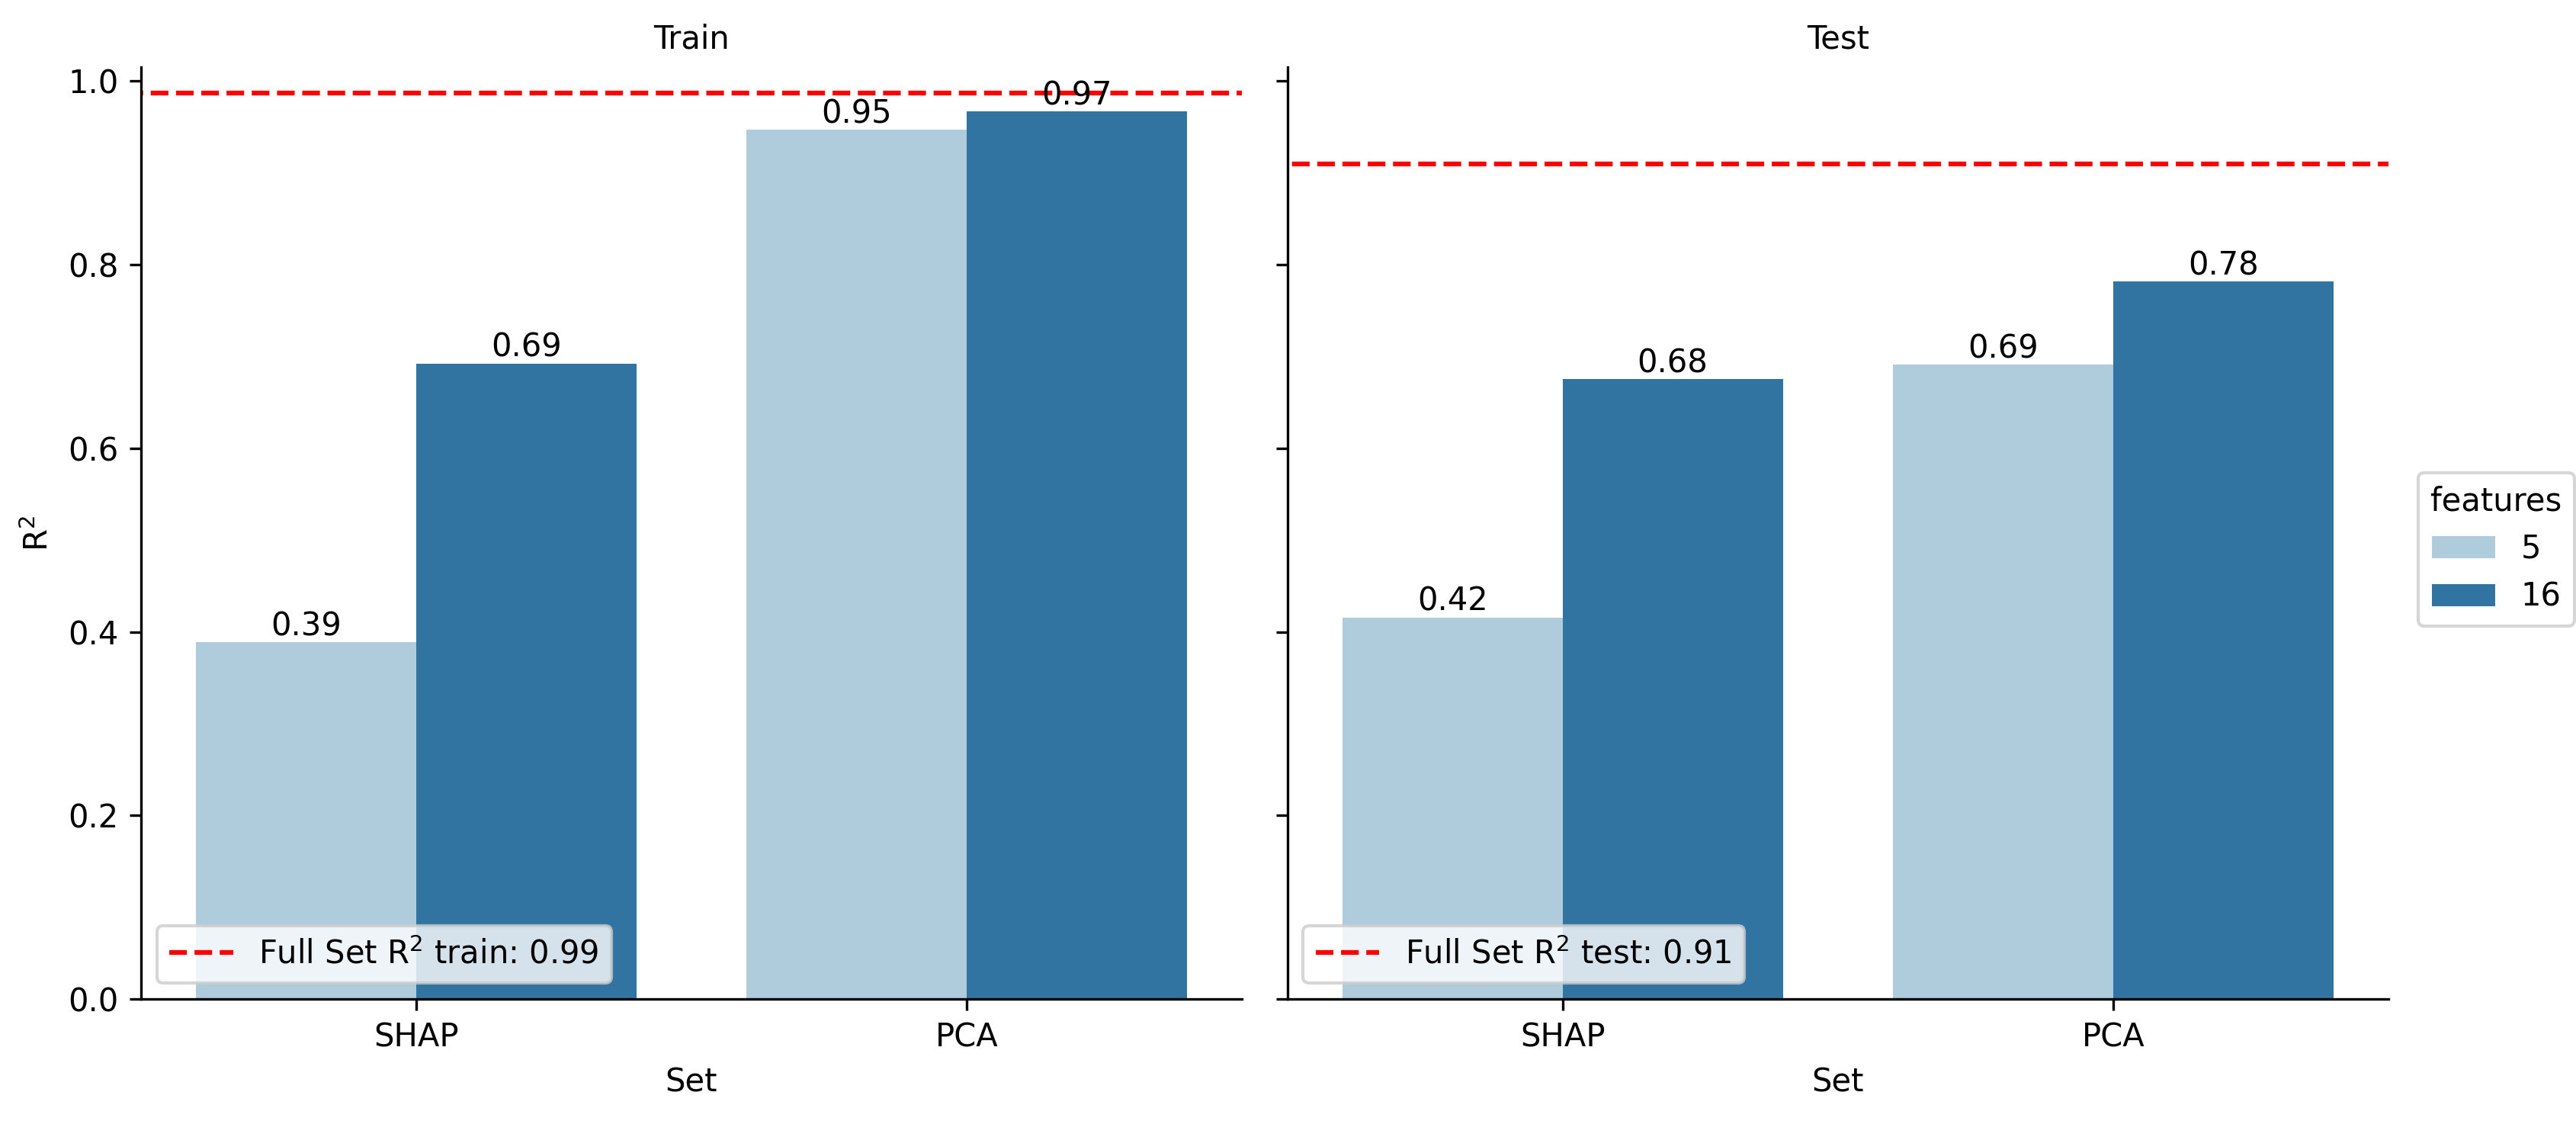
\includegraphics[width=\textwidth]{../images/BSE/classical_features_R2.png}
		\caption{}
		\label{fig:BSE_classical_features_R2}
	\end{subfigure}
	\caption{Feature reduction of the BSE dataset represented using }
	\label{fig:bse_classical_features}
\end{figure}


The next chemical dataset explored is based on the data-driven coupled-cluster (DDCC) method, which is a machine learning-based approach for accelerating the convergence of coupled-cluster singles and doubles (CCSD) calculations.\cite{townsend_data-driven_2019,jones_chapter_2023}
This method works by predicting the $t_{2}$-amplitudes of the CCSD wave function (Eq. \ref{eq:cc_wfn}) with features generated using lower-level methods, such as Hartree-Fock (HF) and M{\o}ller-Plesset second-order perturbation theory (MP2), which are used to initialize CCSD calculations.

The coupled-cluster wave function takes the general form,
\begin{equation}
	\ket{\Psi_{\text{CC}}} = \exp(\hat{T}) \ket{\Psi_{0}}
	\label{eq:cc_wfn}
\end{equation}
where the cluster operator is denoted as $\hat{T}$ and the reference, Hartree-Fock wave function is denoted as $\ket{\Psi_{0}}$.
The CCSD wave function truncates the cluster operator to only include singles and doubles excitations.
The CCSD correlation energy is defined as,
\begin{equation}
	E^{\text{CCSD}}_{\text{corr}} = \sum_{\substack{a<b \\ i<j}} \mel{ij}{}{ab} t^{ab}_{ij} + \sum_{\substack{a<b \\ i<j}} \mel{ij}{}{ab} t^{a}_{i} t^{b}_{j}
	\label{eq:cc_corr}
\end{equation}
where $i$ and $j$ denote occupied orbitals, $a$ and $b$ denote virtual orbitals, $t^{ab}_{ij}$ are the $t_{2}$-amplitudes which correspond to two-electron excitations, 
$t^{a}_{i}$ and $t^{b}_{j}$ are $t_{1}$-amplitudes corresponding to one-electron excitations, and $\mel{ij}{}{ab}$ are two-electron integrals.

For each two-electron excitation, $t^{ab}_{ij}$, a feature set can be generated from HF and MP2.
The feature set includes the MP2 $t_{2}$-amplitudes, which are used to initialize the CCSD amplitudes,
\begin{equation}
	t^{ab}_{ij(\text{MP2})} = \frac{\mel{ij}{}{ab}}{\varepsilon_{i}+\varepsilon_{j}-\varepsilon_{a}-\varepsilon_{b}}
	\label{eq:MP2_t2}
\end{equation}
where $\varepsilon_{i}$ and $\varepsilon_{j}$ denote the orbital energies of the occupied orbitals $i$ and $j$, while the virtual orbitals $a$ and $b$ are denoted by $\varepsilon_{a}$ and $\varepsilon_{b}$.
Features related to the MP2 $t_{2}$-amplitudes that are also included in the feature set are the numerator ($\mel{ij}{}{ab}$) and denominator ($\varepsilon_{i}+\varepsilon_{j}-\varepsilon_{a}-\varepsilon_{b}$), a binary feature to denote whether the excitation goes to the same virtual orbital, and the orbital energies ($\varepsilon_{i},\varepsilon_{j},\varepsilon_{a},\varepsilon_{b}$).
The feature set also includes terms related to the individual contributes to the orbital energies are also included, such as the one-electron Hamiltonain ($h$), Coulombic matrix ($J$), and exchange matrix $K$, and Coulombic and exchange integrals ($J^{i}_{a},J^{j}_{b},K^{a}_{i},K^{b}_{j}$).
In total, there are 30 features for each $t_{2}$-amplitude due to the addition of features that denote the sign and magntudes of the previously mentioned features.

Our dataset consists of 199 water molecules from the study by Townsend and Vogiatzis using the STO-3G basis set\cite{hehre_selfconsistent_1970} and frozen core orbitals.
All data was generated using Psi4\cite{parrish_psi4_2017} and Psi4Numpy\cite{smith_psi4numpy_2018}.
As previously mentioned, the DDCC method is data intensive regarding the number of samples per molecule, for example, each water molecule has 4 occupied and 2 virtual orbitals.
The number of $t_{2}$-amplitudes is equivalent to $(N_{occ})^{2}(N_{virt})^{2}$, where $N_{occ}$ denotes the number of occupied orbitals and $N_{virt}$ denotes the number of virtual orbitals, so the total number of $t_{2}$-amplitudes per molecule is 64.
Further details regarding the feature set and implementation can be found in \cite{townsend_data-driven_2019}

Like the BSE dataset, the 30 features from the full DDCC feature set must be reduced to 5 or 16 features using SHAP or PCA.
Unlike the BSE dataset, we choose SHAP over PCA for the feature reduction since there is a direct correlation between the input features and output values.
As shown in Fig. \ref{fig:DDCC_feature_set}, 5 and 16 features can accurately recover performance of the original model using 30 features, where all three models have train and test R$^{2}$s of 1.00.
Due to the computational costs of running QML models, we will then use only 5 features for all DDCC QML models.
The 5 most important features are the two-electron integrals ($\mel{ij}{}{ab}$), MP2 $t_{2}$-amplitudes ($t^{ab}_{ij(\text{MP2})}$), the magnitude of the MP2 $t_{2}$-amplitudes, and the difference in orbital energies ($\varepsilon_{i}+\varepsilon_{j}-\varepsilon_{a}-\varepsilon_{b}$).



\begin{figure}[H]
	\centering
	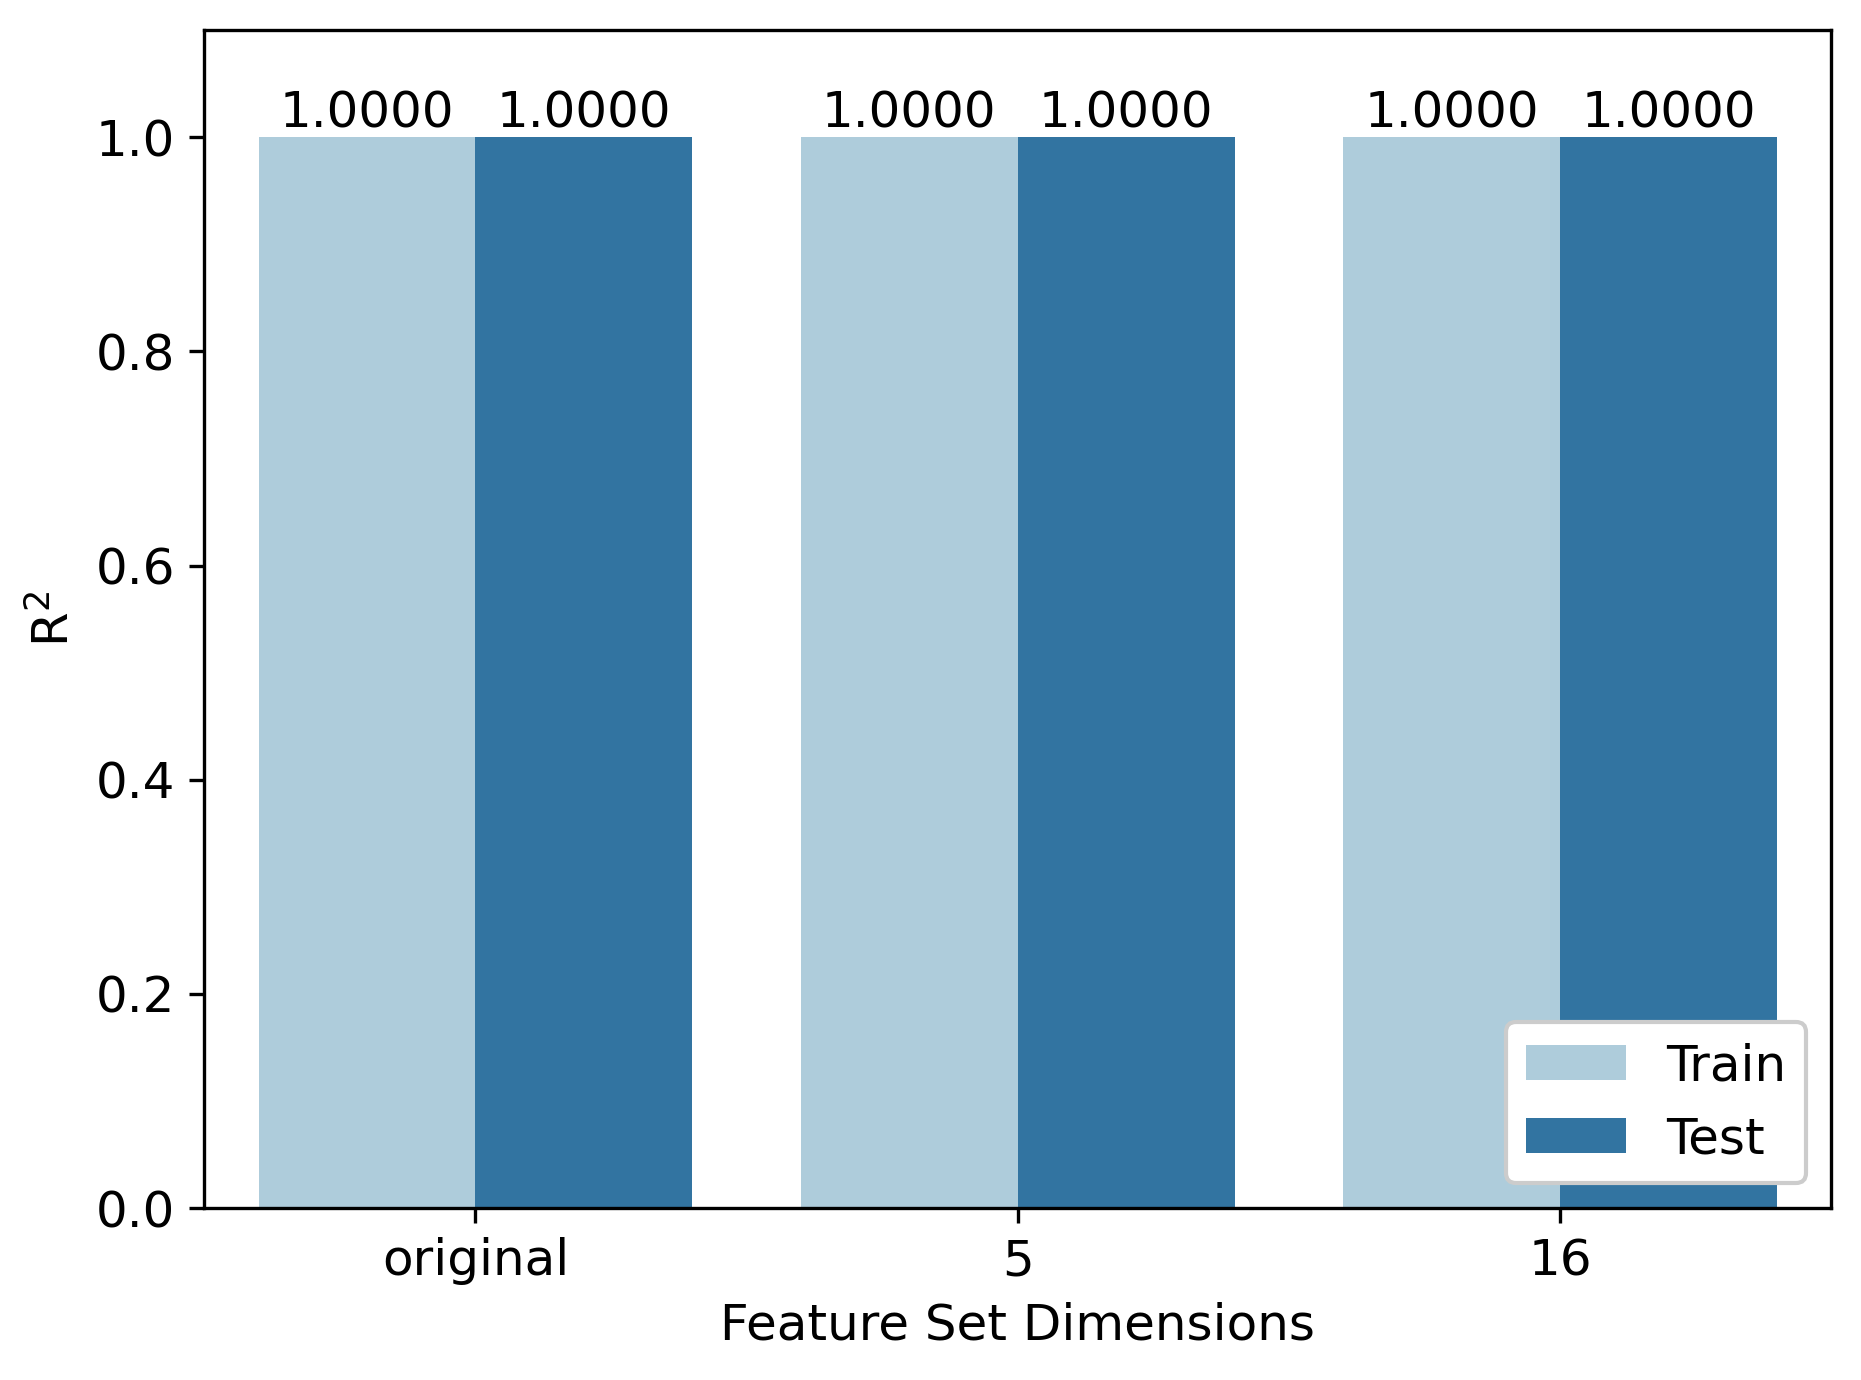
\includegraphics[width=0.49\textwidth]{../images/DDCC/DDCC_feature_set.png}
	\caption{}
	\label{fig:DDCC_feature_set}
\end{figure}


% Make distribution plot
%\begin{figure}[H]
%	\centering
%	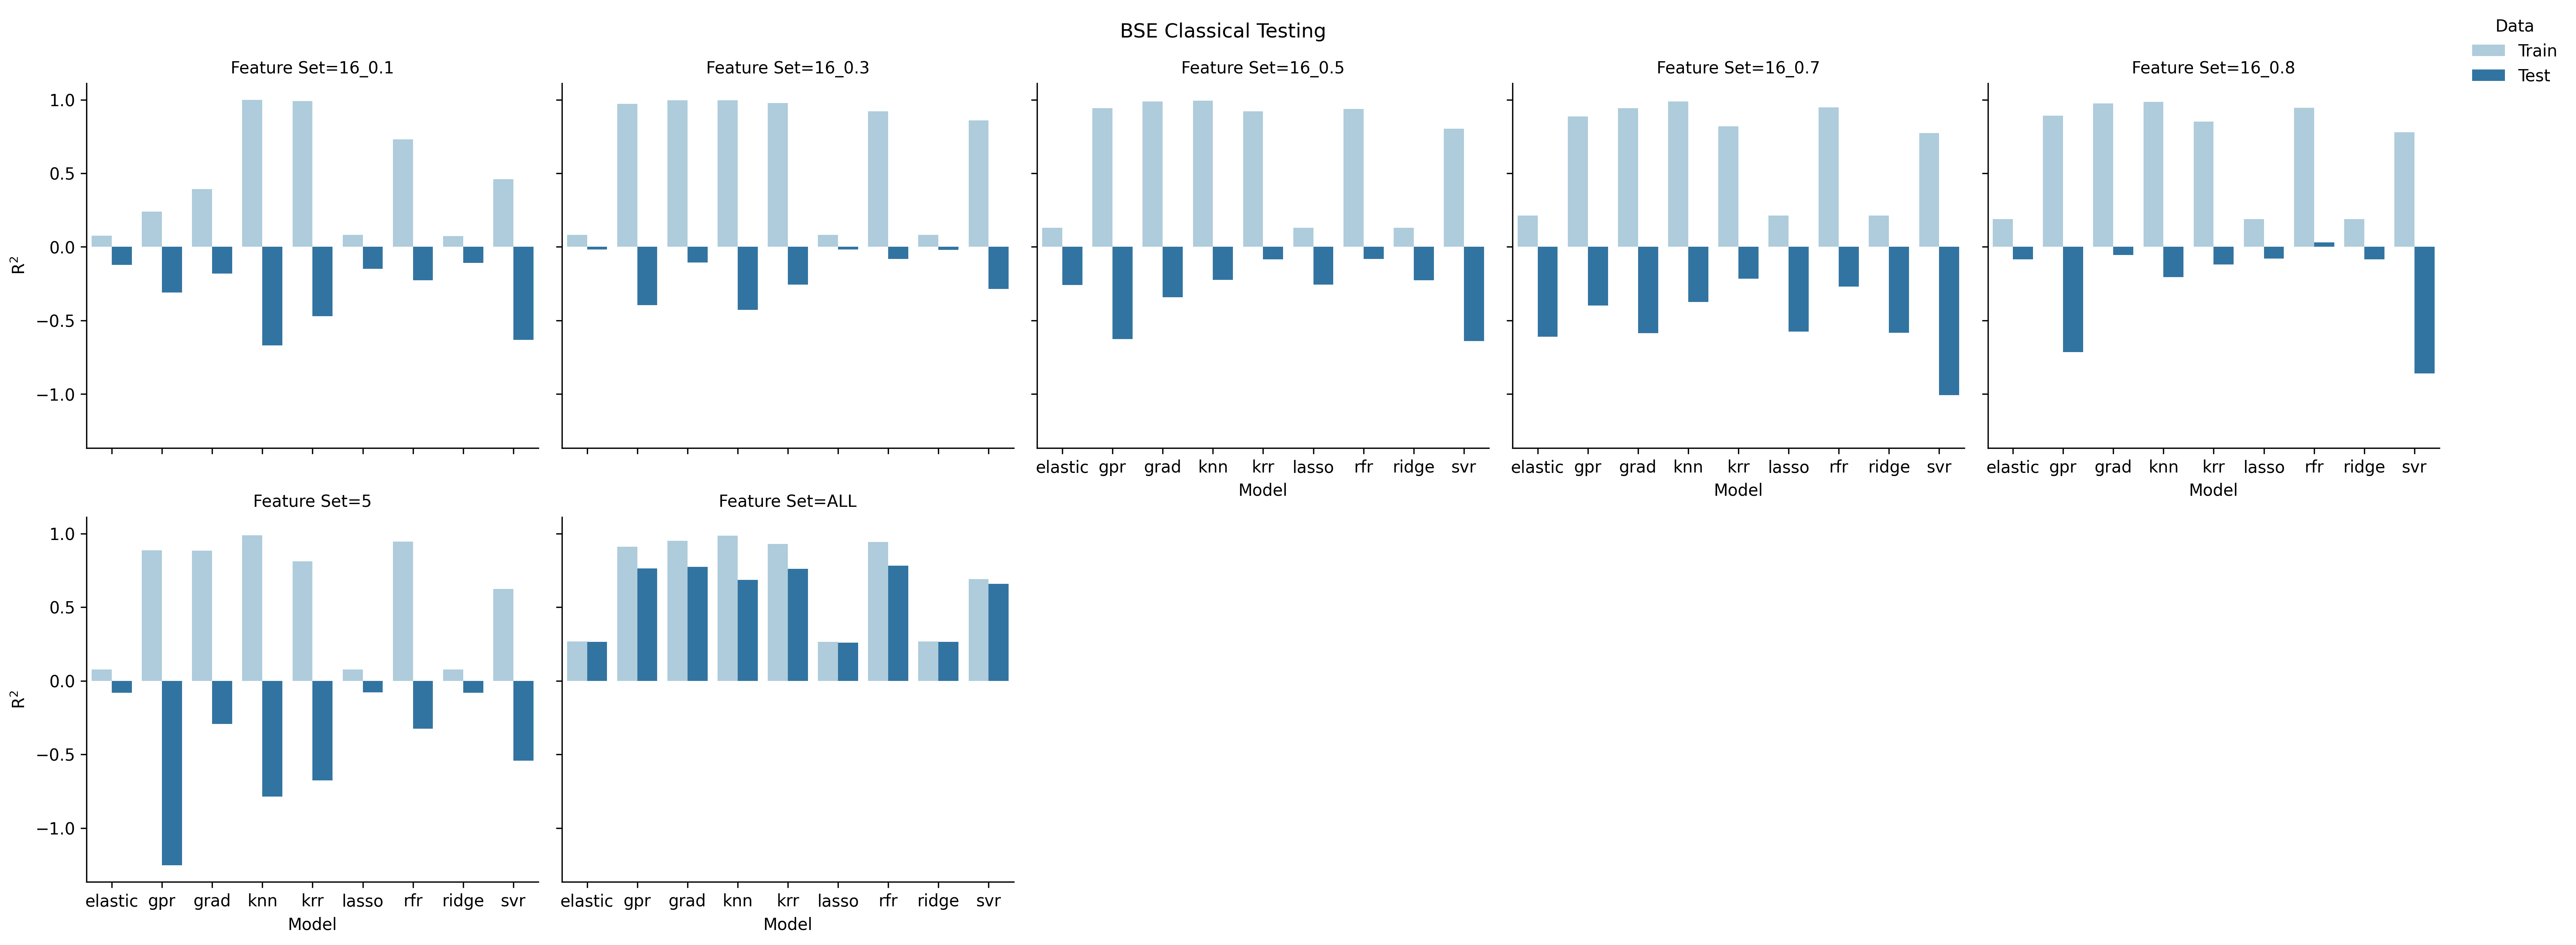
\includegraphics[width=\linewidth]{../images/BSE.png}
%	\caption{BSE}
%	\label{fig:BSE}
%\end{figure}







\section{Results and Discussion}
\label{section:results_and_discussion}


\subsection{BSE}
To explore the performance of PQCs for chemically relevant datasets, the dataset we explore is the BSE49 dataset, which consists of a diverse set of bond separation energies and the related structures, as highlighted in Figs. \ref{fig:bondtypes} and \ref{fig:BSEdistr}.
Initially, we study the five qubit data, Figs. \ref{fig:5BSE_heatplots} and \ref{fig:5BSE_boxplots}, due to computational considerations.



five qubit 
best encoder-ansatz pair: train R$^{2}$/test R$^{2}$
Best encoder on average train R$^{2}$/test R$^{2}$
Best ansatz on average train R$^{2}$/test R$^{2}$

'M-M-CNOT', '-0.0216'
'Full-CRX', '0.1214'

sixteen qubit \ref{fig:16BSE_heatplots} \ref{fig:16BSE_boxplots}
removed the really bad ones from five qubit
best encoder-ansatz pair: train R$^{2}$/test R$^{2}$
Best encoder on average train R$^{2}$/test R$^{2}$
Best ansatz on average train R$^{2}$/test R$^{2}$


Talk about the cost of going wider, and inherently deeper


\begin{figure}[H]
	\centering	
	\begin{subfigure}[b]{0.49\textwidth}
		\centering
		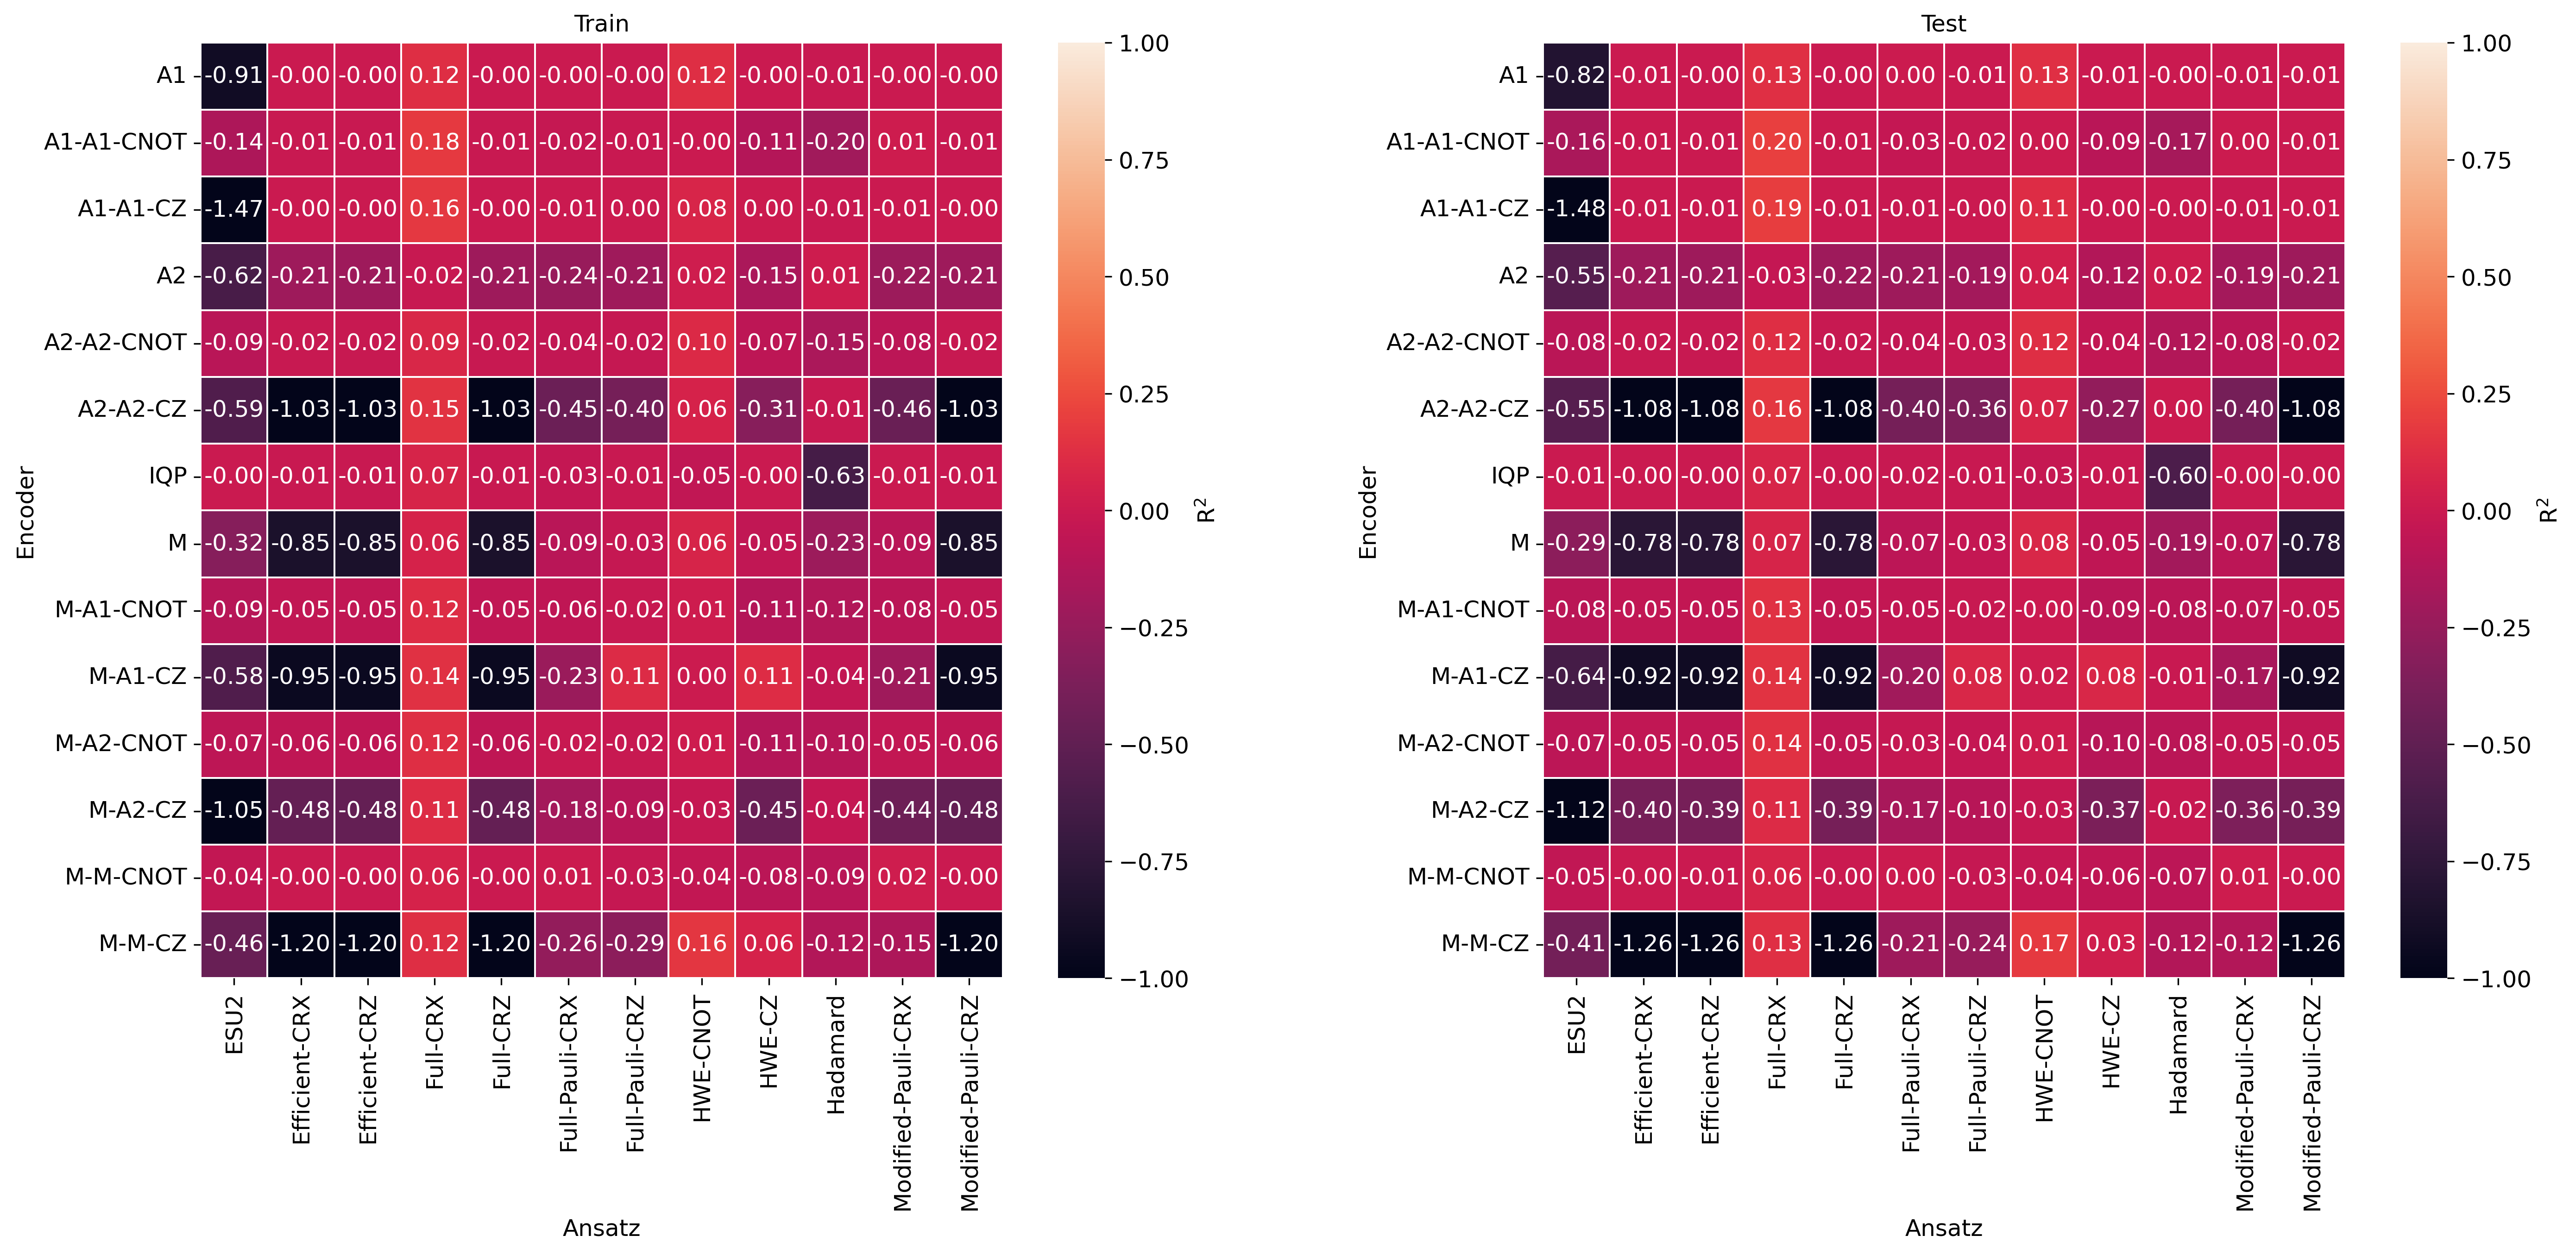
\includegraphics[width=\linewidth]{../images/BSE/fivequbit/BSE_heatplots}
		\caption{}
		\label{fig:5BSE_heatplots}
	\end{subfigure}
	\hfill
	\begin{subfigure}[b]{0.49\textwidth}
		\centering
		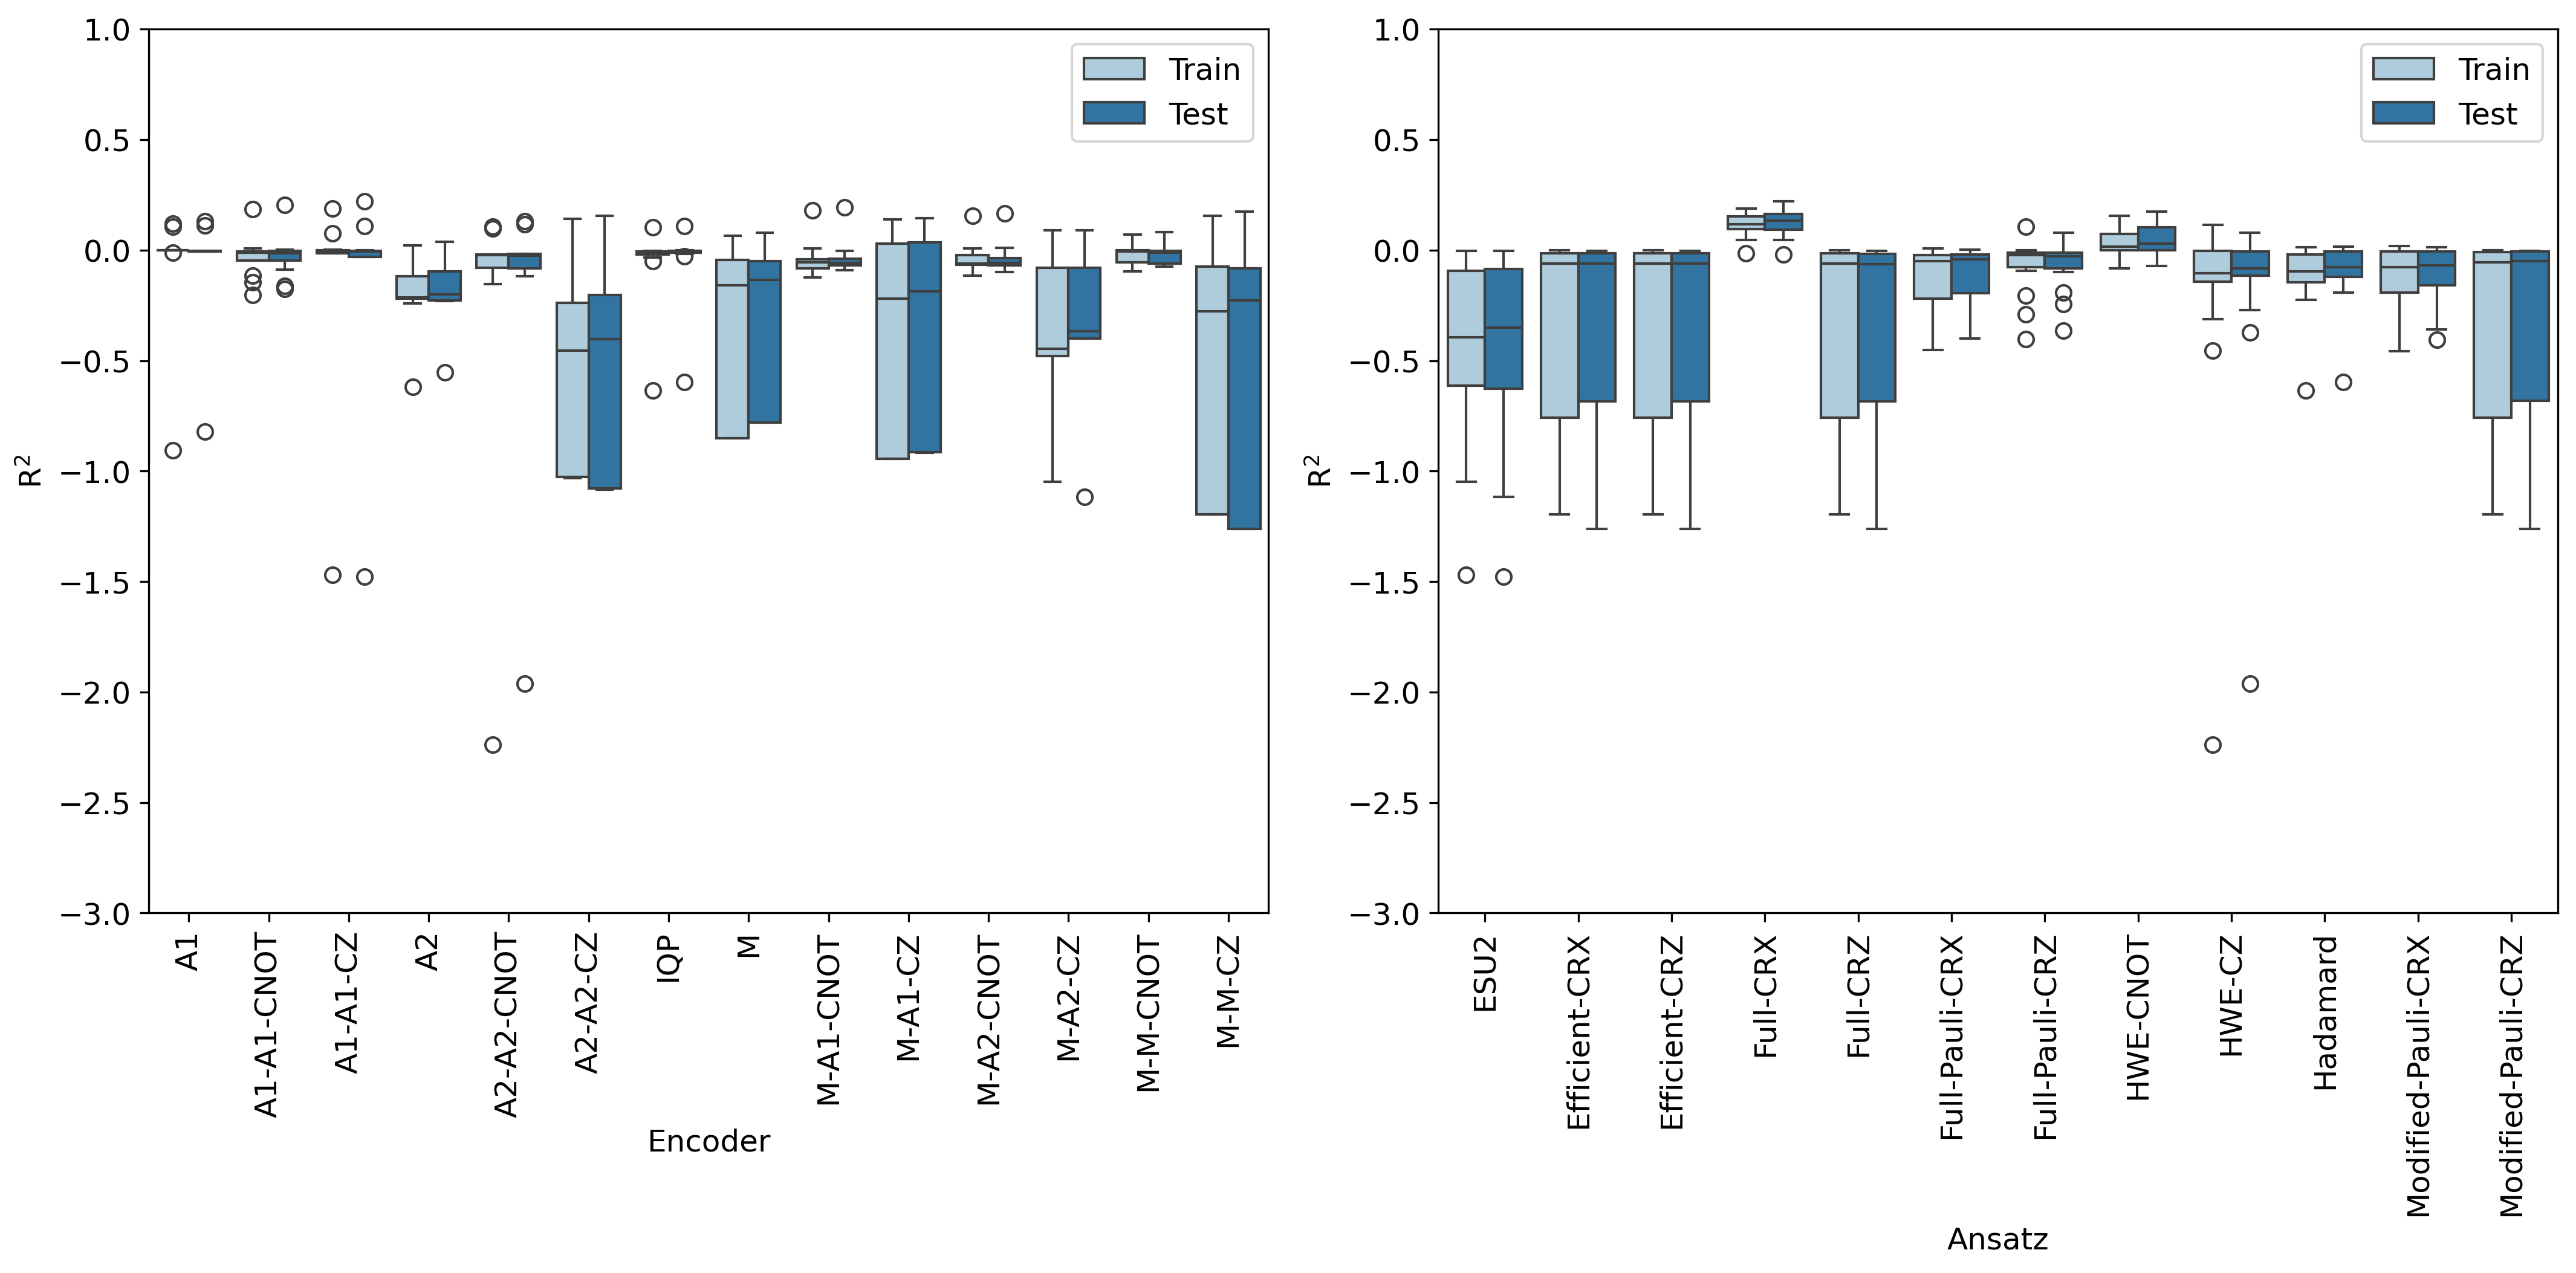
\includegraphics[width=\linewidth]{../images/BSE/fivequbit/BSE_boxplots}
		\caption{}
		\label{fig:5BSE_boxplots}
	\end{subfigure}
	\hfill
	\begin{subfigure}[b]{0.49\textwidth}
		\centering
		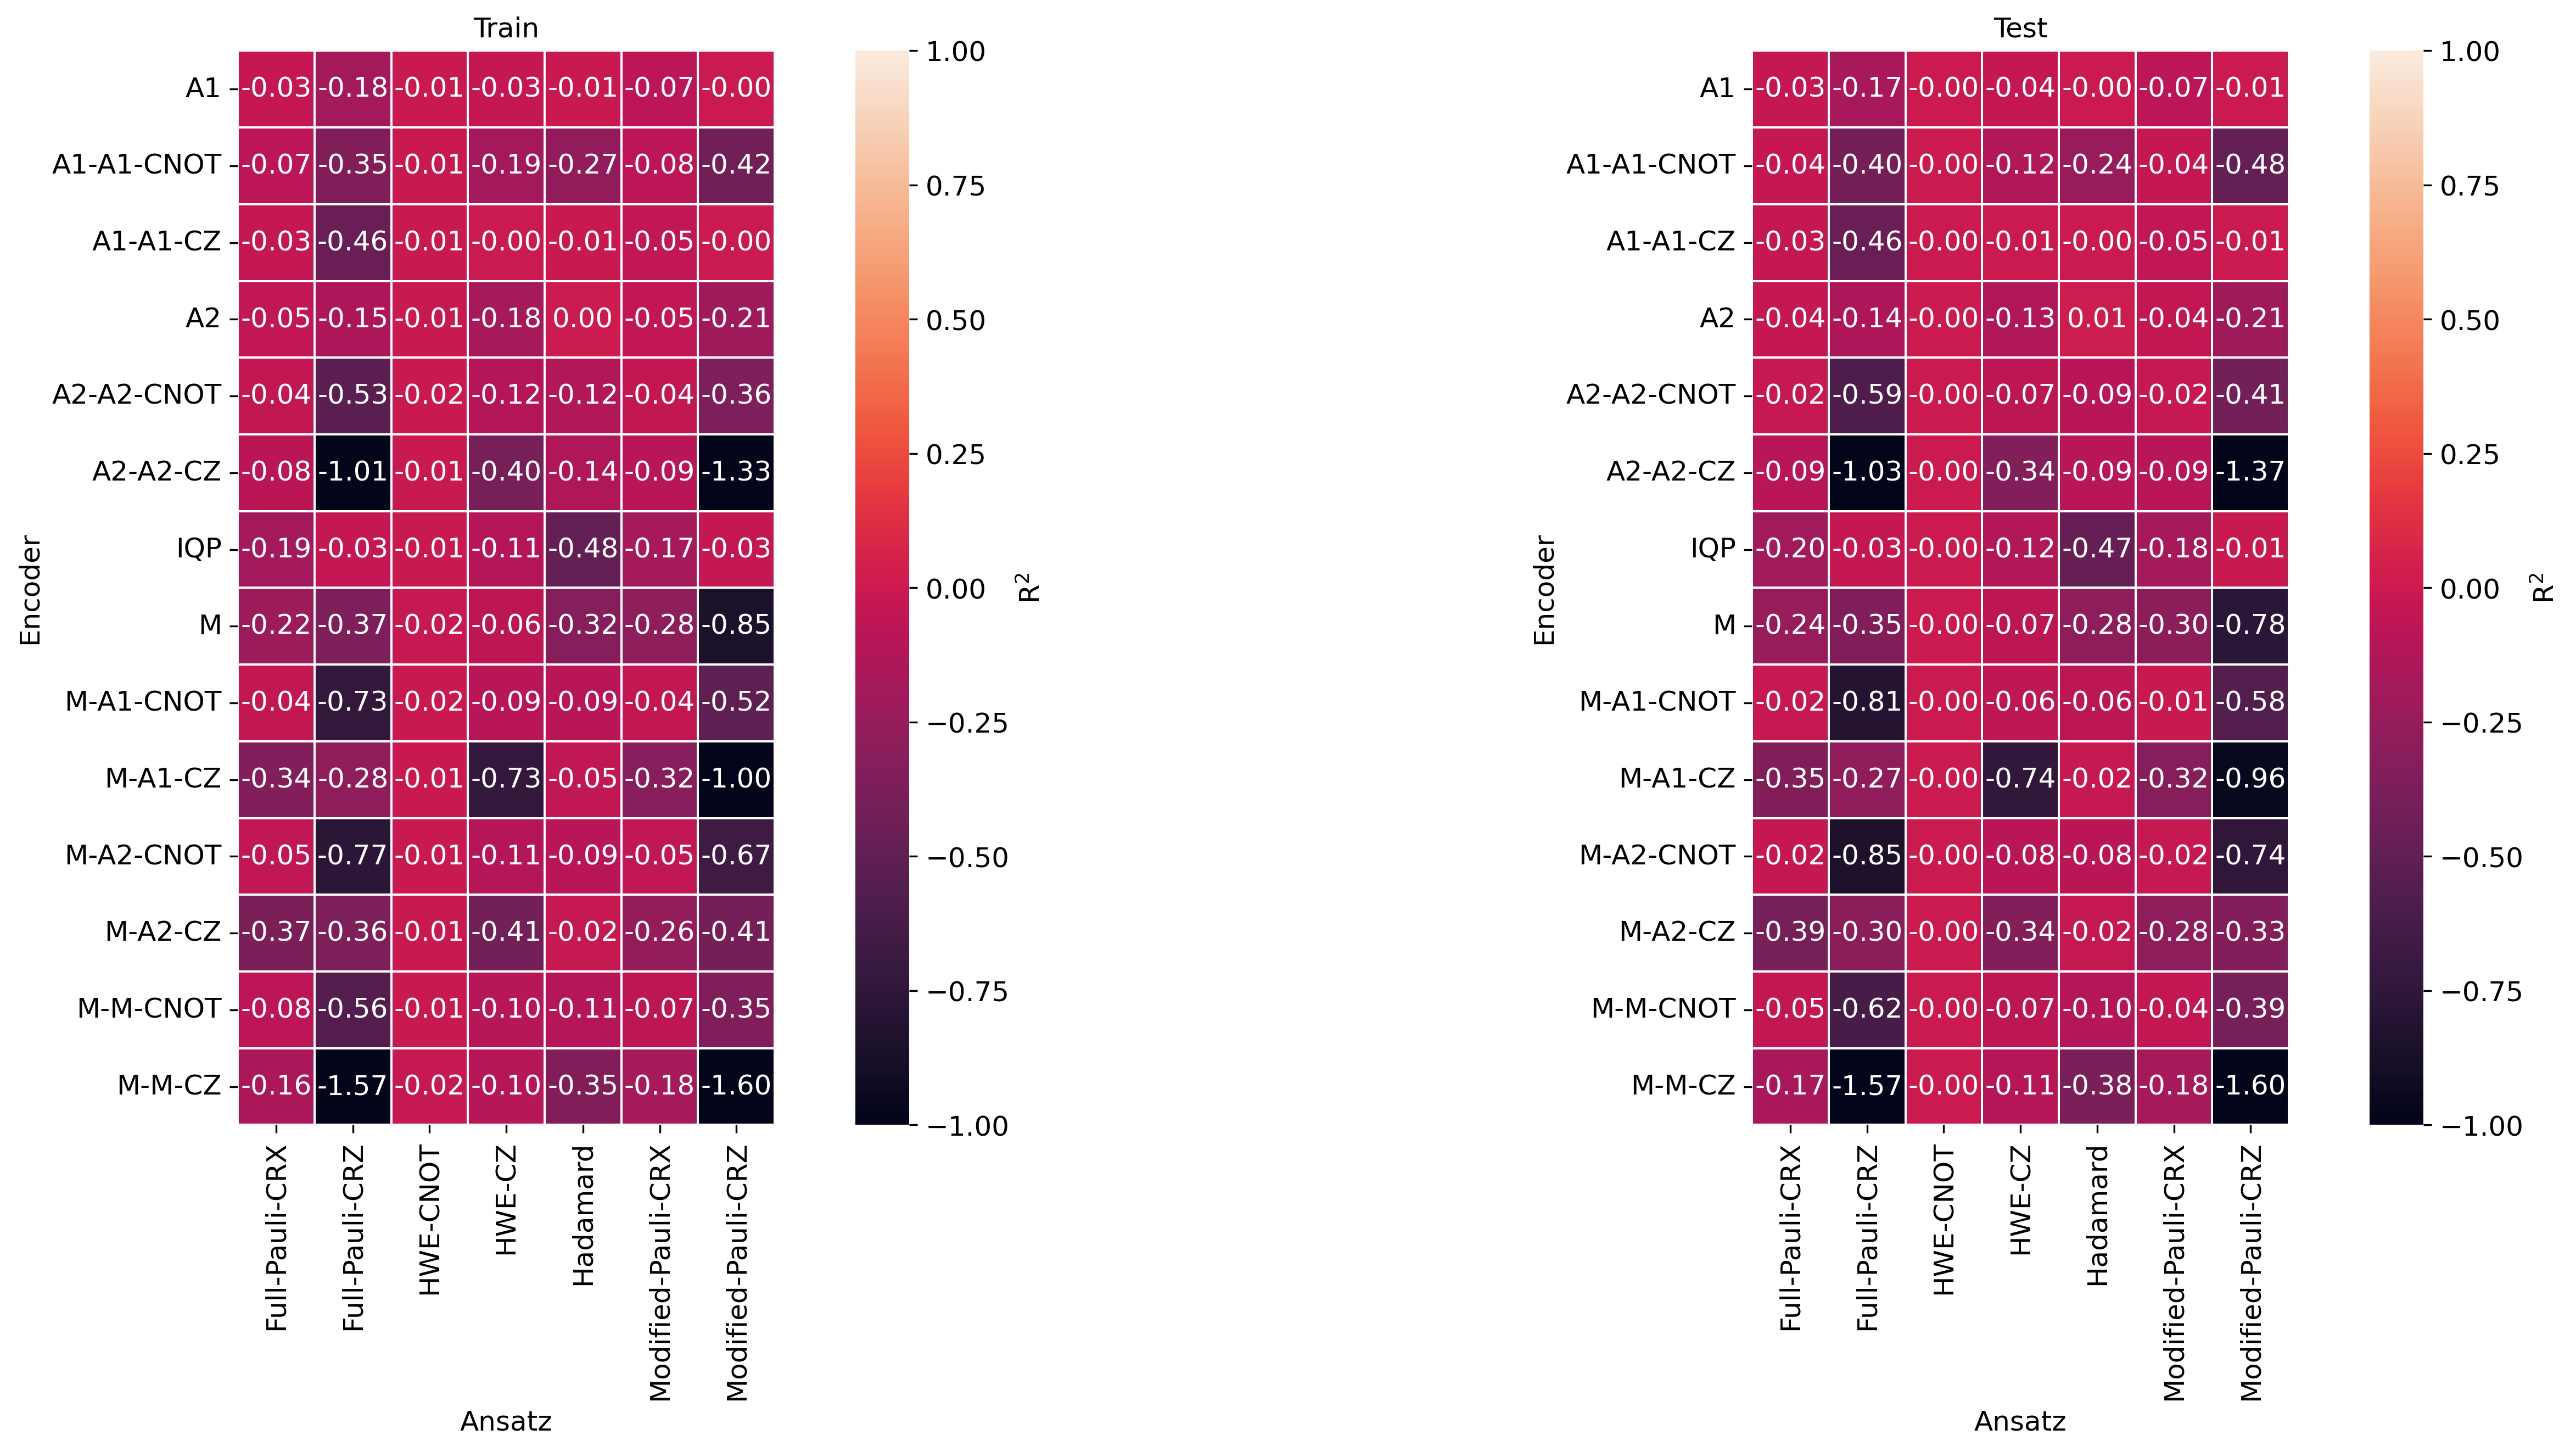
\includegraphics[width=\linewidth]{../images/BSE/sixteenqubit/BSE_heatplots}
		\caption{}
		\label{fig:16BSE_heatplots}
	\end{subfigure}
	\hfill
	\begin{subfigure}[b]{0.49\textwidth}
		\centering
		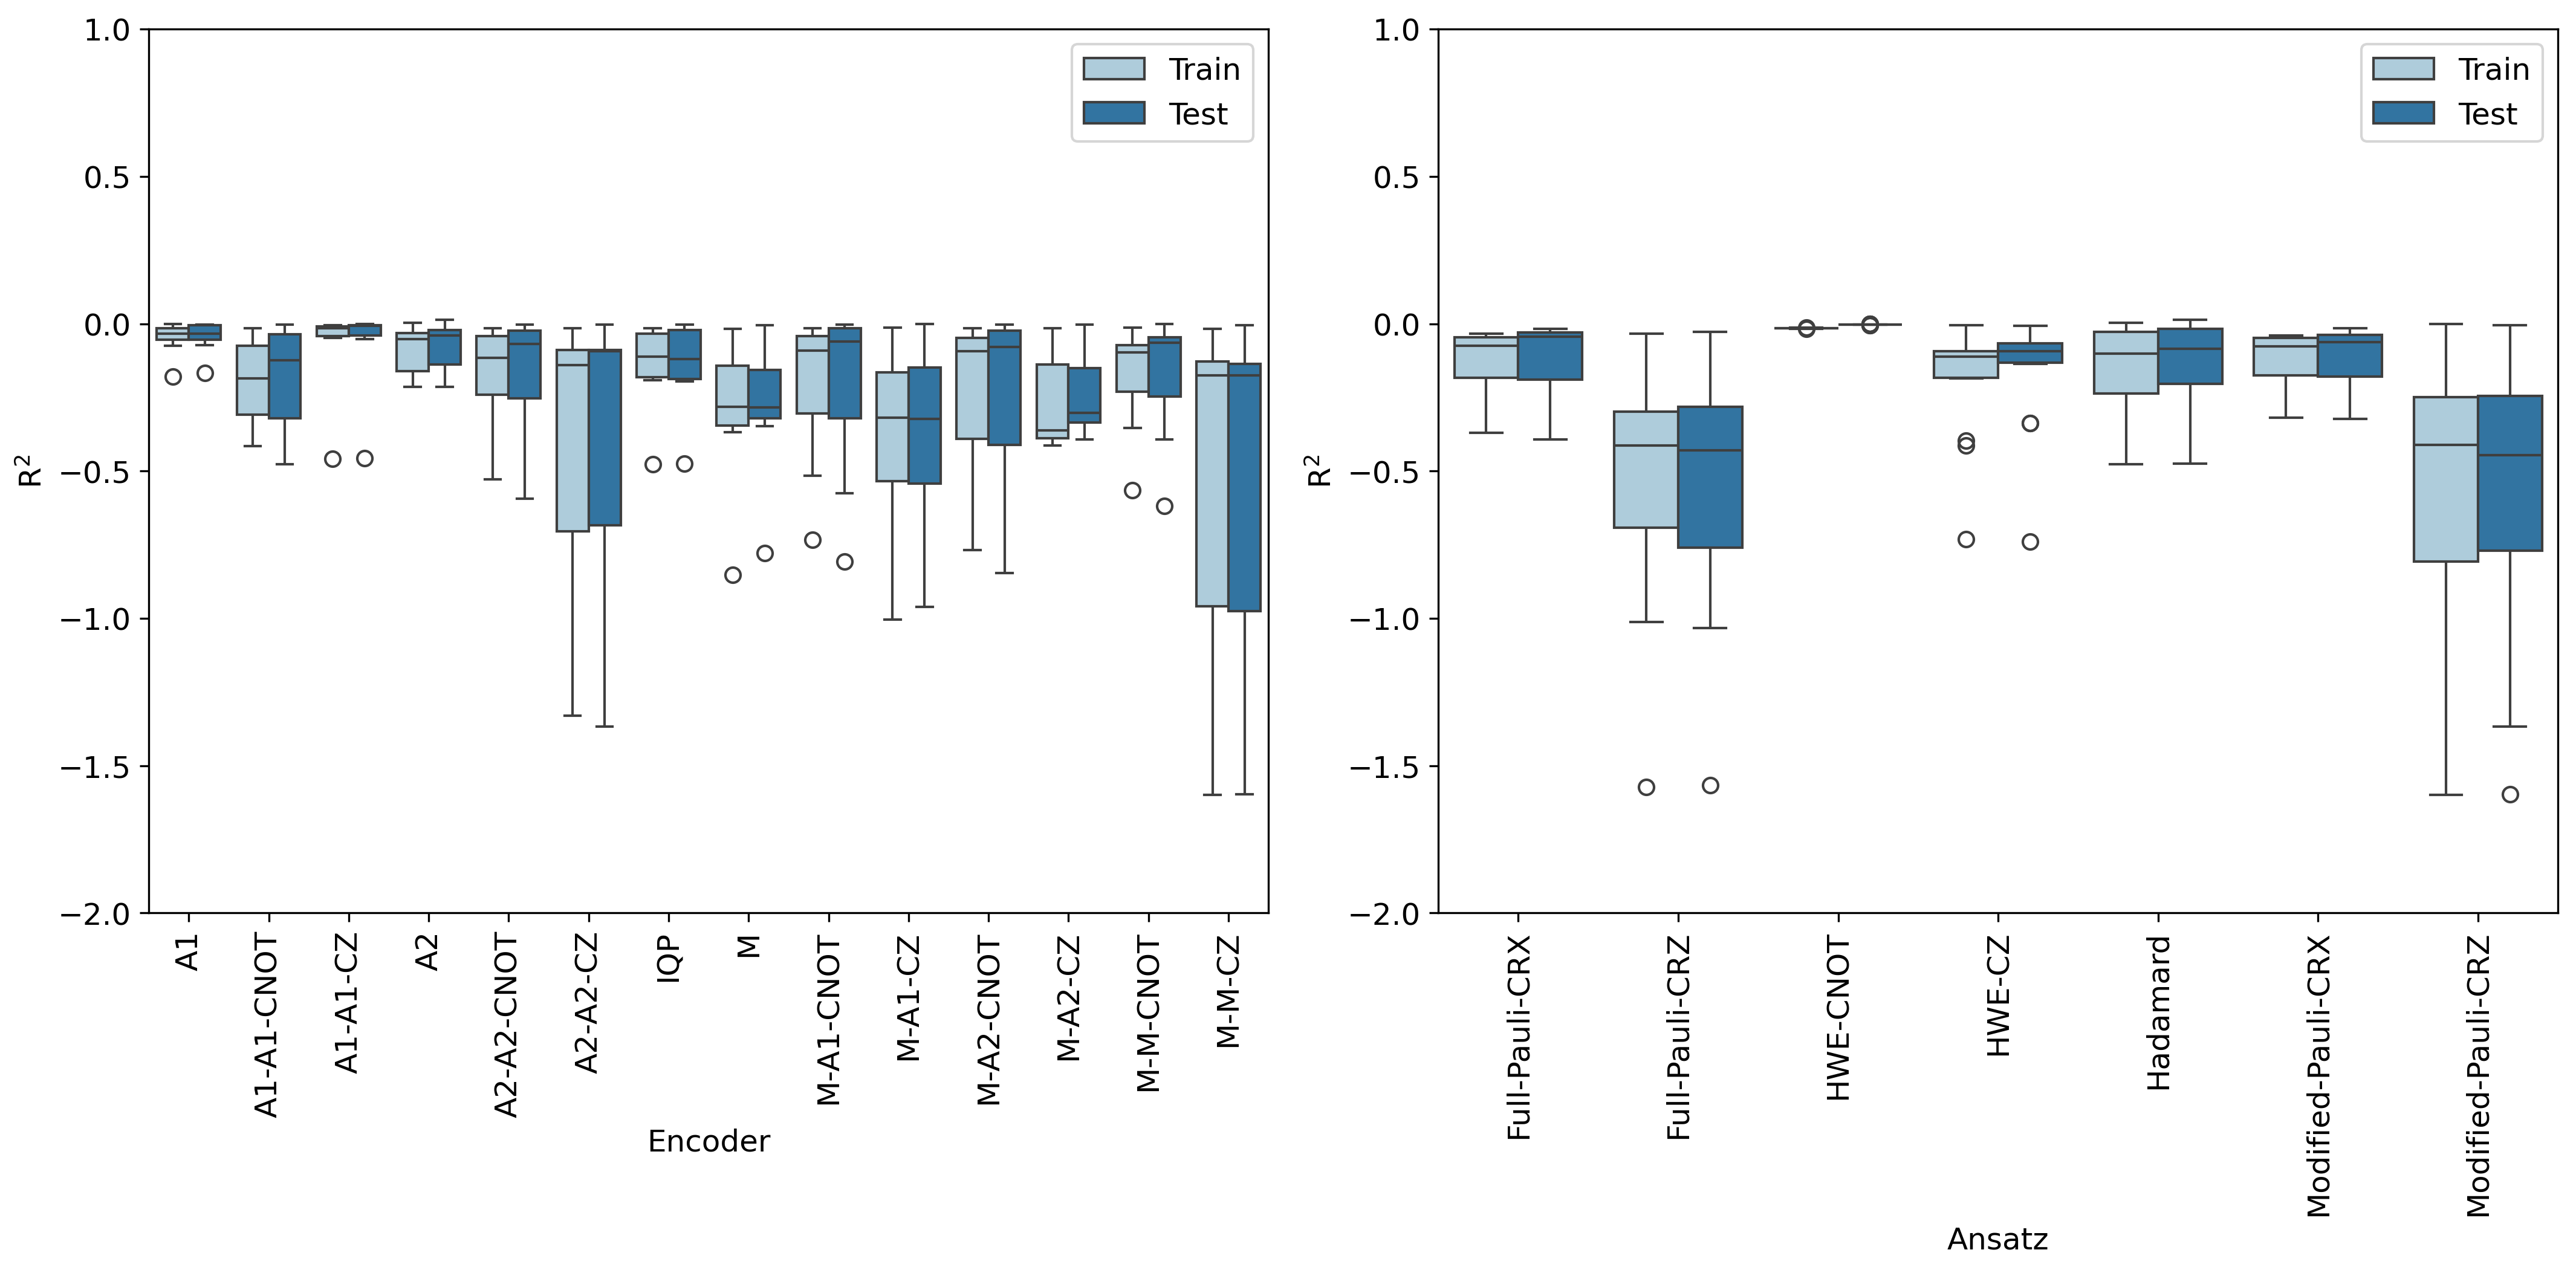
\includegraphics[width=\linewidth]{../images/BSE/sixteenqubit/BSE_boxplots}
		\caption{}
		\label{fig:16BSE_boxplots}
	\end{subfigure}
	\caption{}
	\label{fig:BSEboxandheat}	
\end{figure}

\begin{figure}[H]
	\centering	
	\begin{subfigure}[b]{0.49\textwidth}
		\centering
		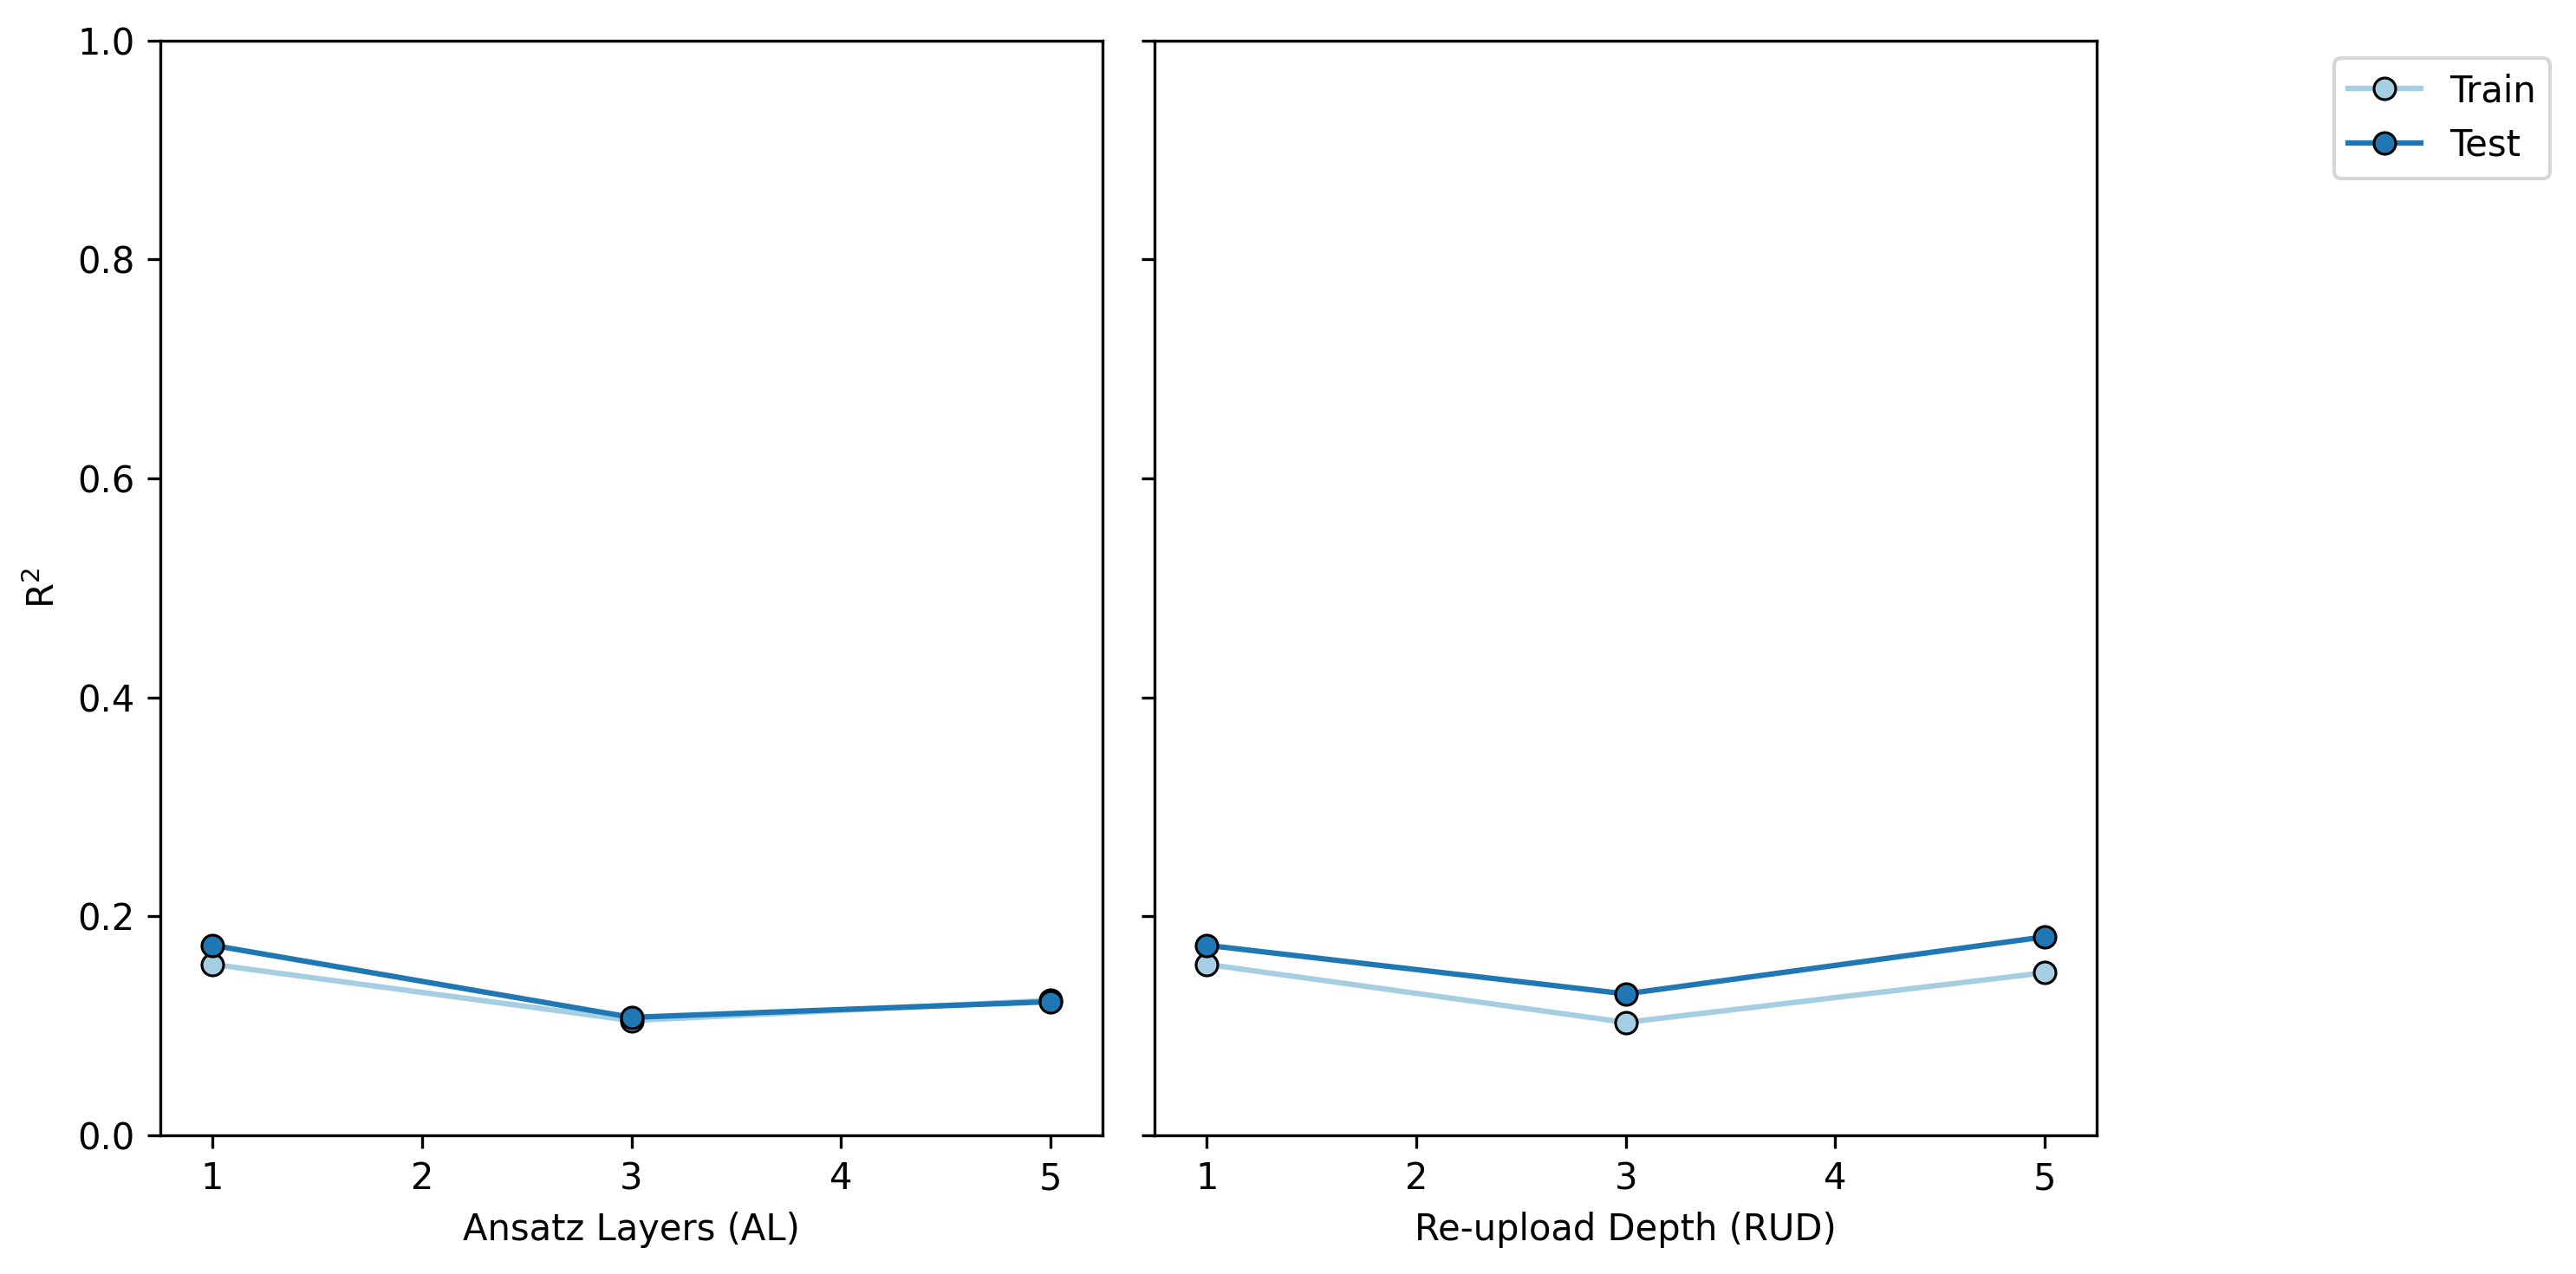
\includegraphics[width=\linewidth]{../images/BSE/fivequbit/BSE5_RUDAL_lineplot}
		\caption{}
		\label{fig:bse5RUDAL_lineplot}
	\end{subfigure}
	\hfill
	\begin{subfigure}[b]{0.49\textwidth}
		\centering
		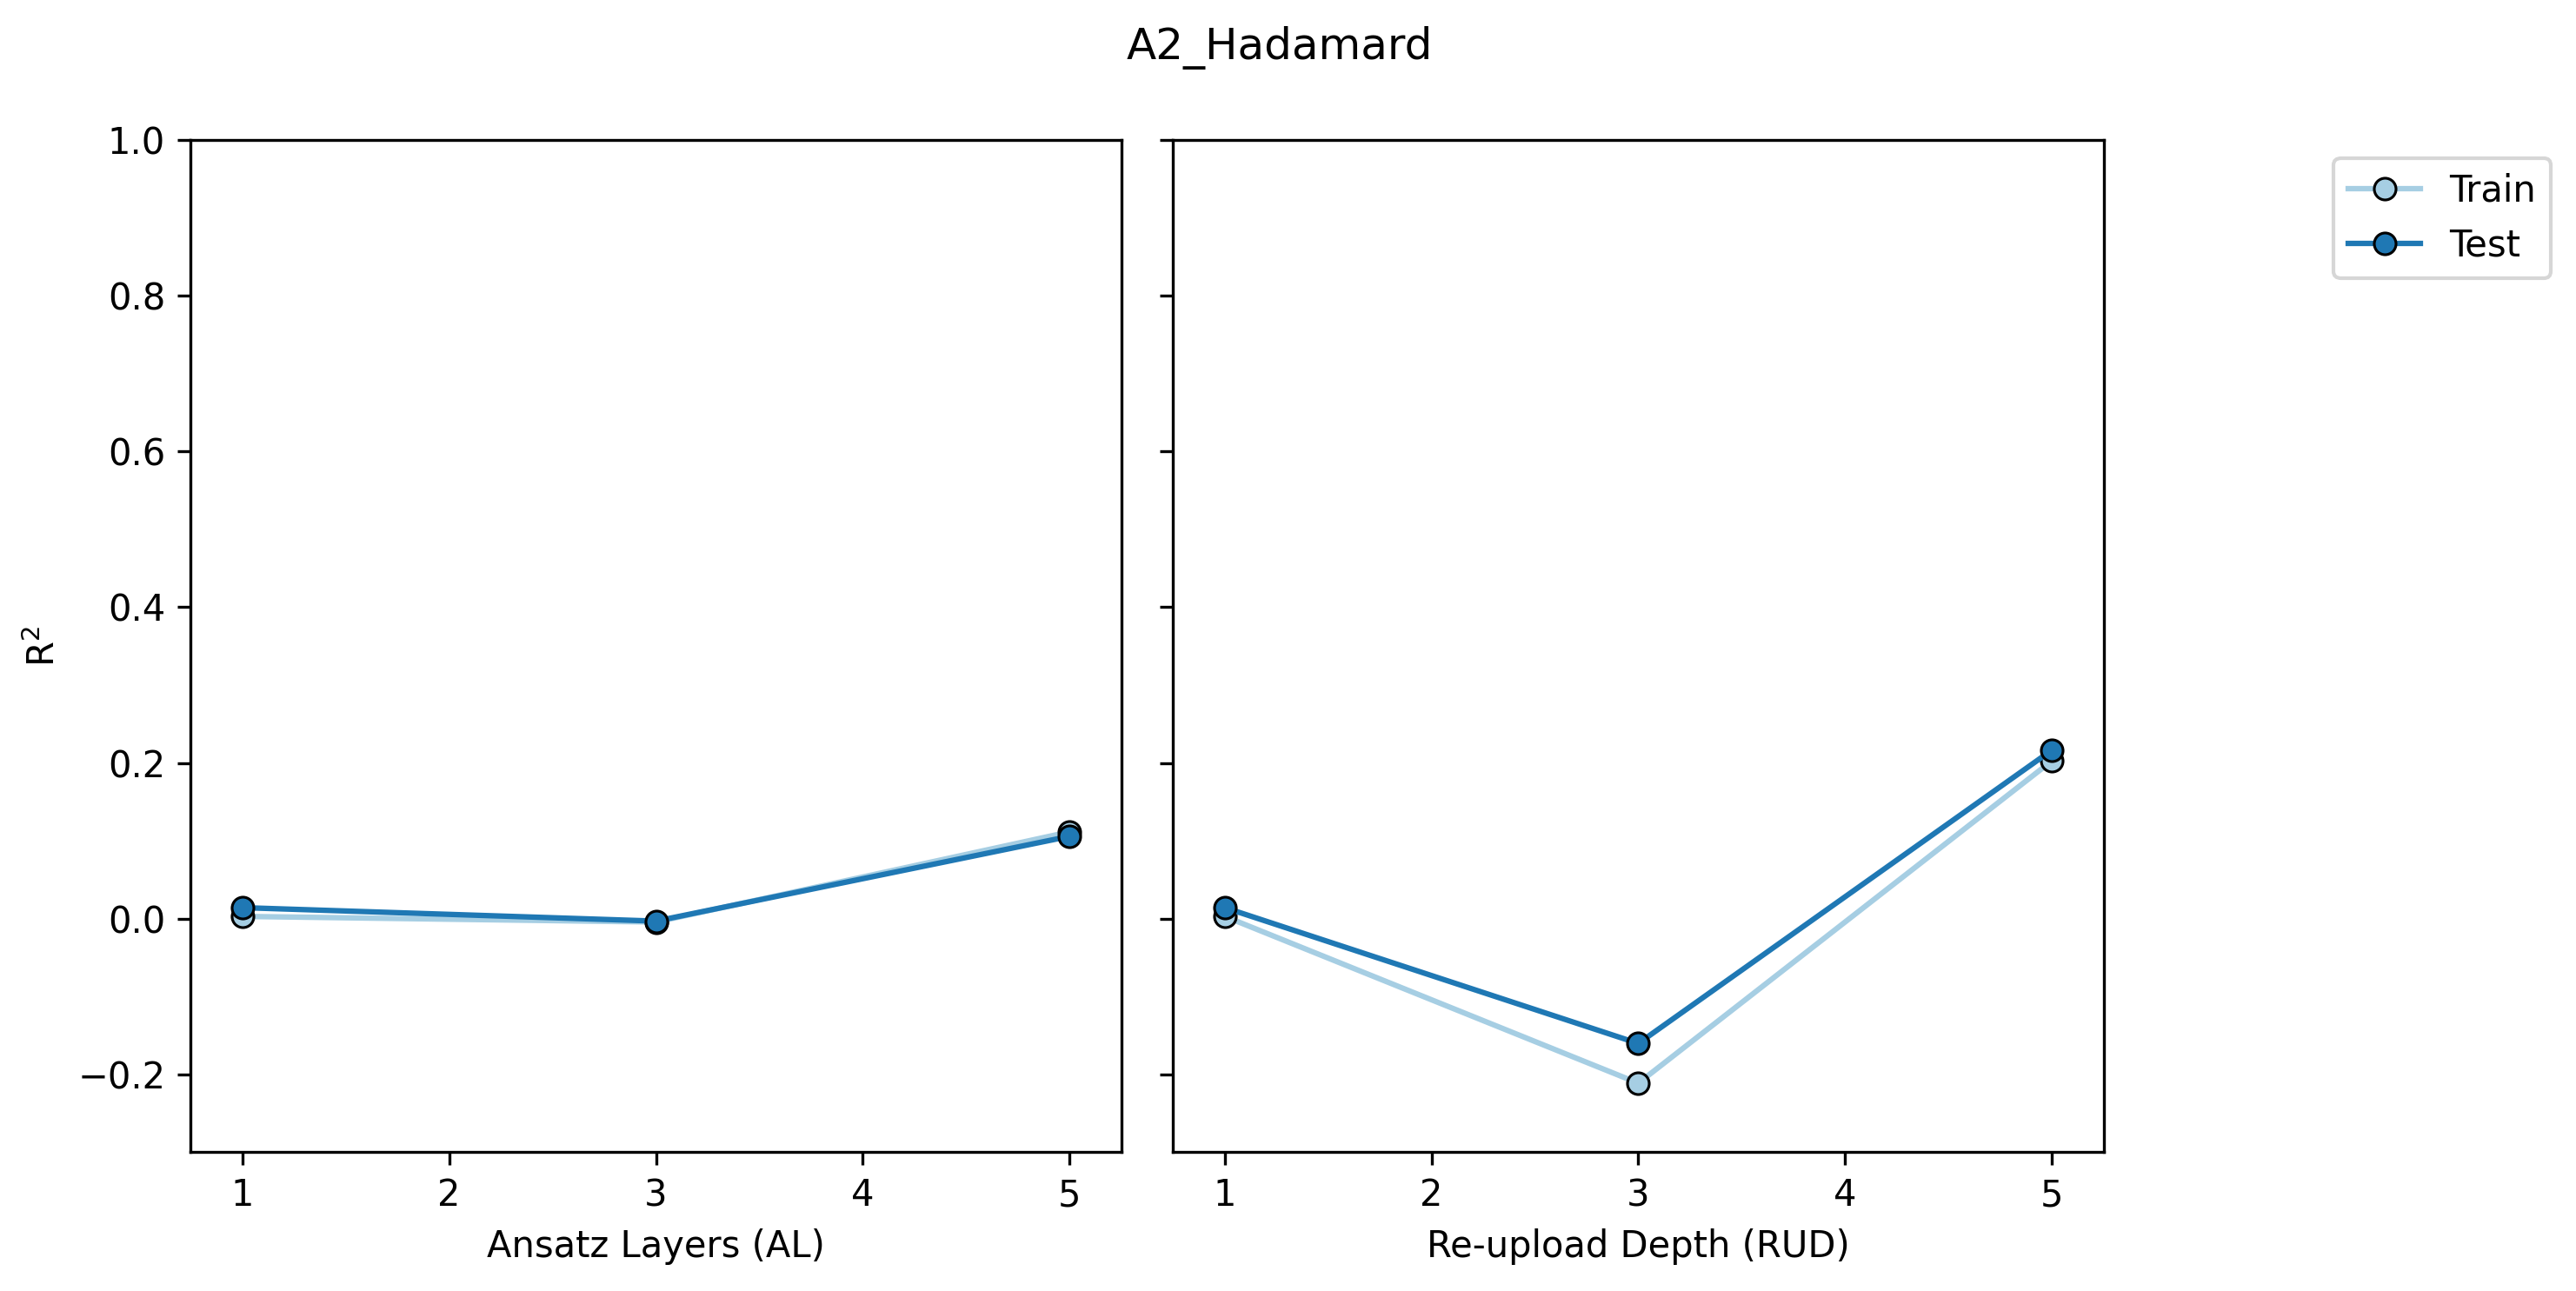
\includegraphics[width=\linewidth]{../images/BSE/sixteenqubit/BSE16_RUDAL_lineplot}
		\caption{}
		\label{fig:bse16RUDAL_lineplot}
	\end{subfigure}
	\hfill
	\begin{subfigure}[b]{0.49\textwidth}
		\centering
		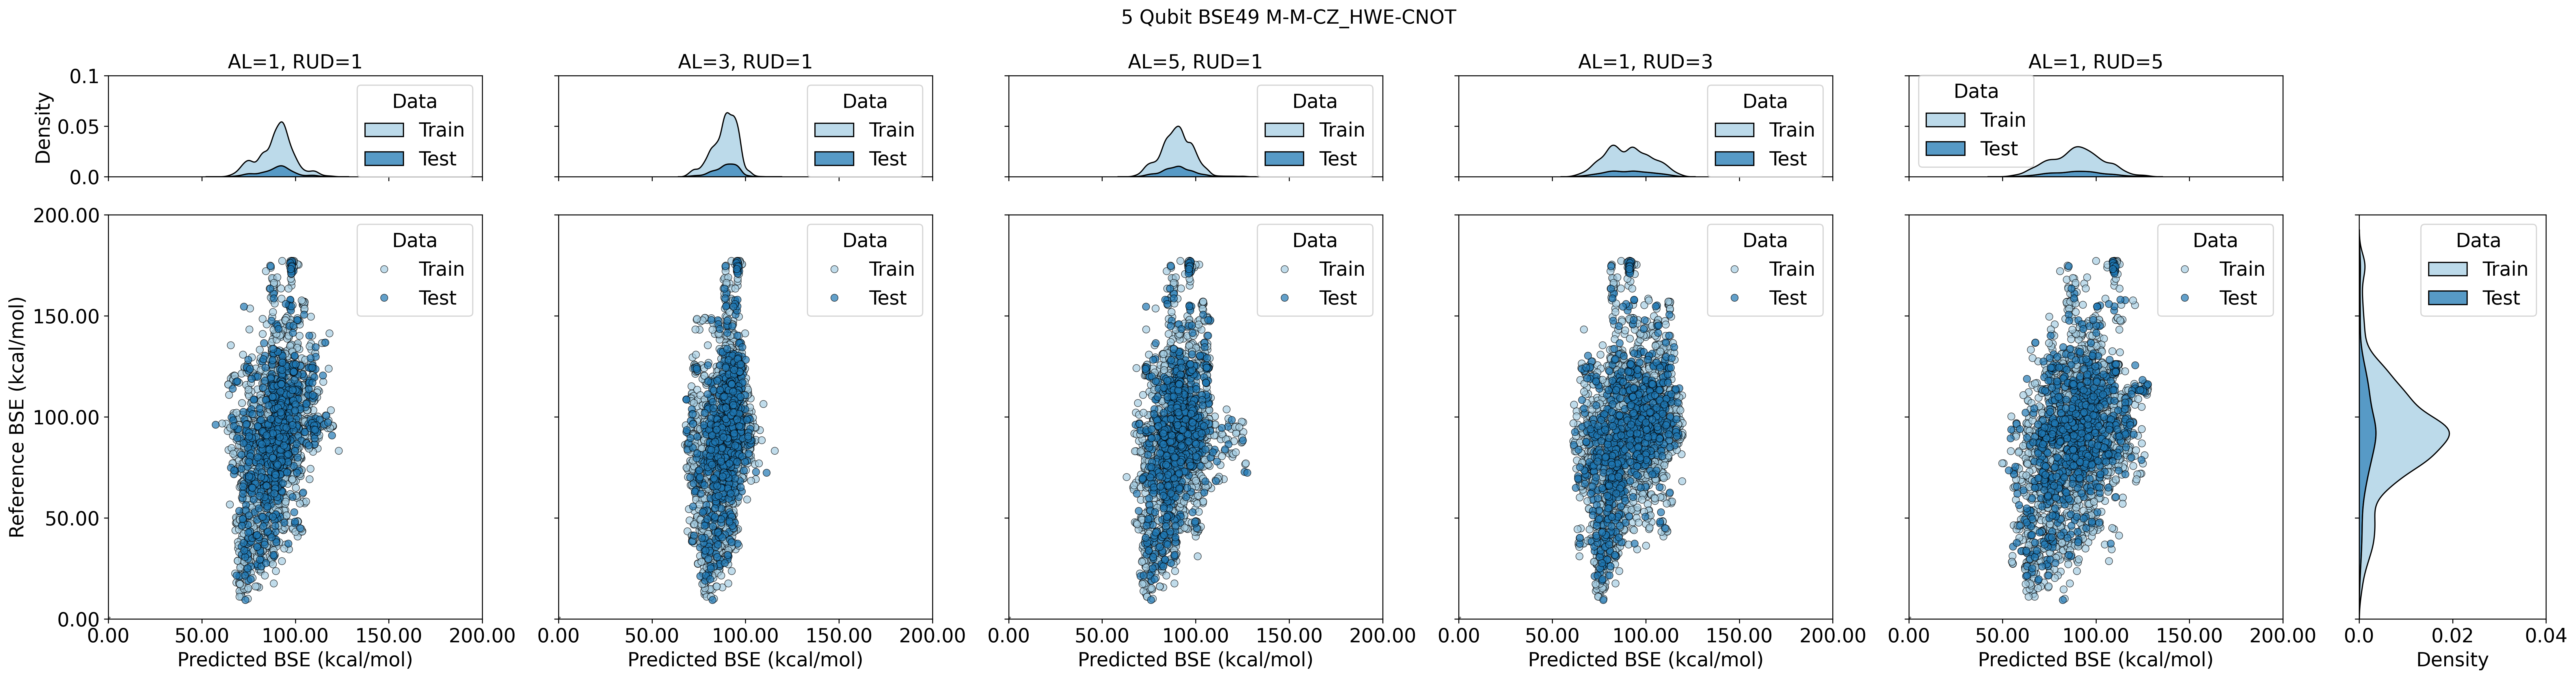
\includegraphics[width=\linewidth]{../images/BSE/fivequbit/distribution_parity}
		\caption{}
		\label{fig:BSE5_distribution_parity}
	\end{subfigure}
	\hfill
	\begin{subfigure}[b]{0.49\textwidth}
		\centering
		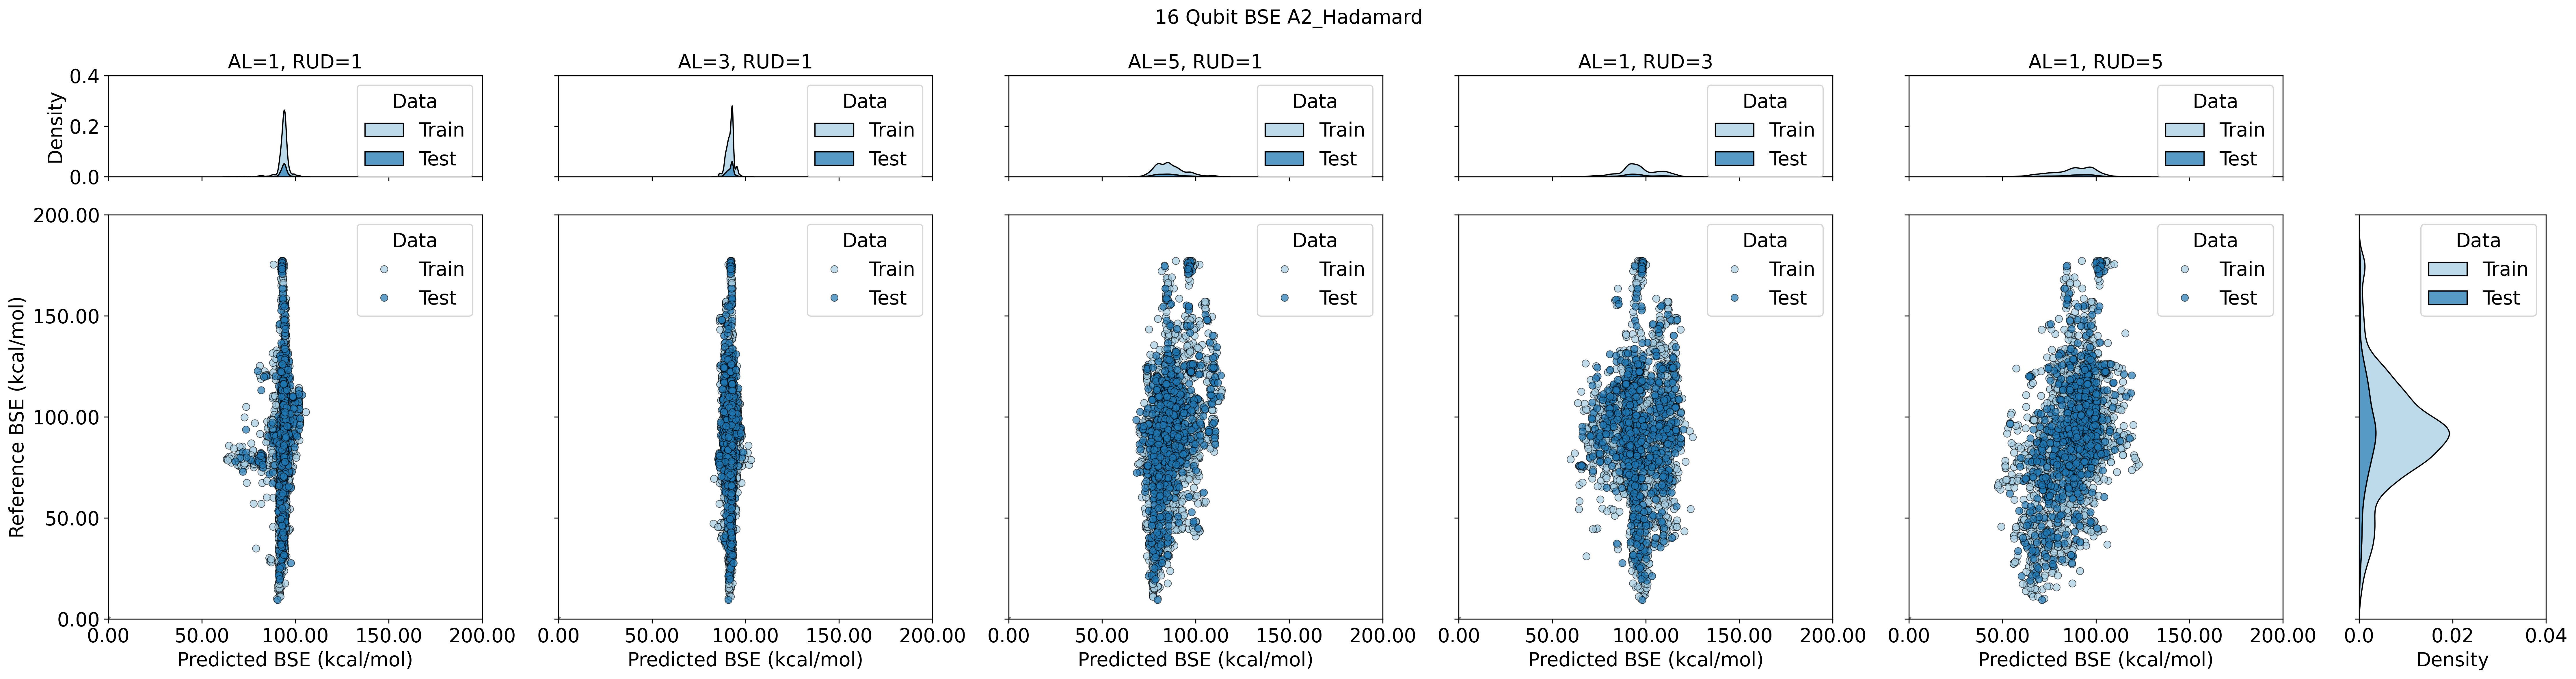
\includegraphics[width=\linewidth]{../images/BSE/sixteenqubit/distribution_parity}
		\caption{}
		\label{fig:BSE16_distribution_parity}
	\end{subfigure}
	\caption{}
	\label{fig:BSE_distribution_parity}	
\end{figure}



\begin{figure}[H]
	\centering	
	\begin{subfigure}[b]{0.49\textwidth}
		\centering
		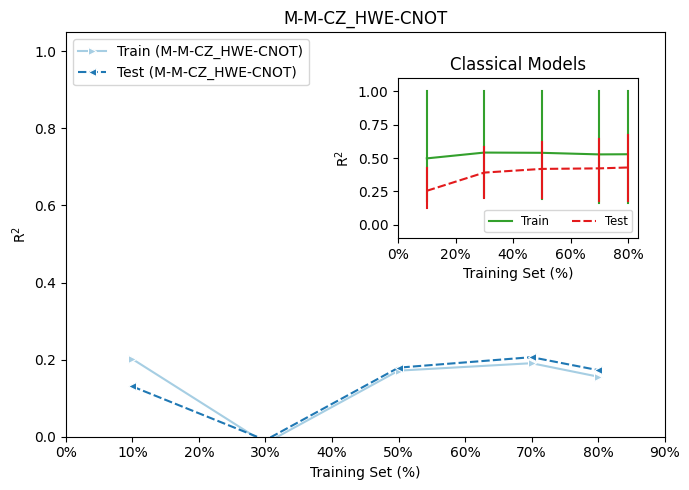
\includegraphics[width=\linewidth]{../images/BSE/fivequbit/BSE_learningcurve}
		\caption{}
		\label{fig:BSE5_learning_curves}
	\end{subfigure}
	\hfill
	\begin{subfigure}[b]{0.49\textwidth}
		\centering
		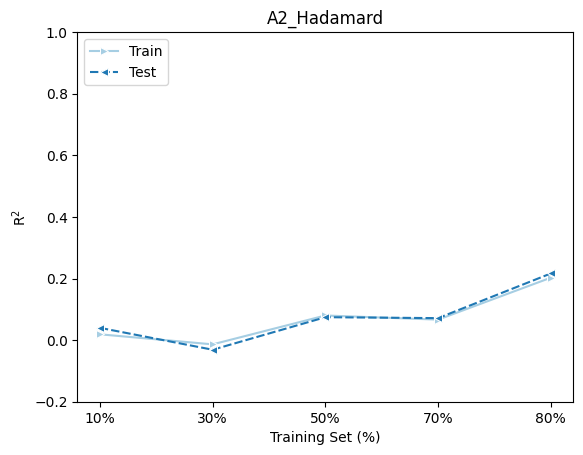
\includegraphics[width=\linewidth]{../images/BSE/sixteenqubit/BSE_learningcurve}
		\caption{}
		\label{fig:BSE16_learningcurve}
	\end{subfigure}
	\caption{}
	\label{fig:BSE_LC}	
\end{figure}







\subsection{DDCC}
Structure
\begin{itemize}
	\item Broad set
	\item RUD/AL tests
	\item learning curve (maybe)
	\item real device 
\end{itemize}

A2\_HWE-CNOT Train R$^{2}$ 0.62/test R$^{2}$ 0.62 
Best encoder average Train R$^{2}$ X/test R$^{2}$ Y
Best ansatz HWE-CNOT average Train R$^{2}$ X/test R$^{2}$ Y

\begin{figure}[H]
	\centering	
	\begin{subfigure}[b]{0.49\textwidth}
		\centering
		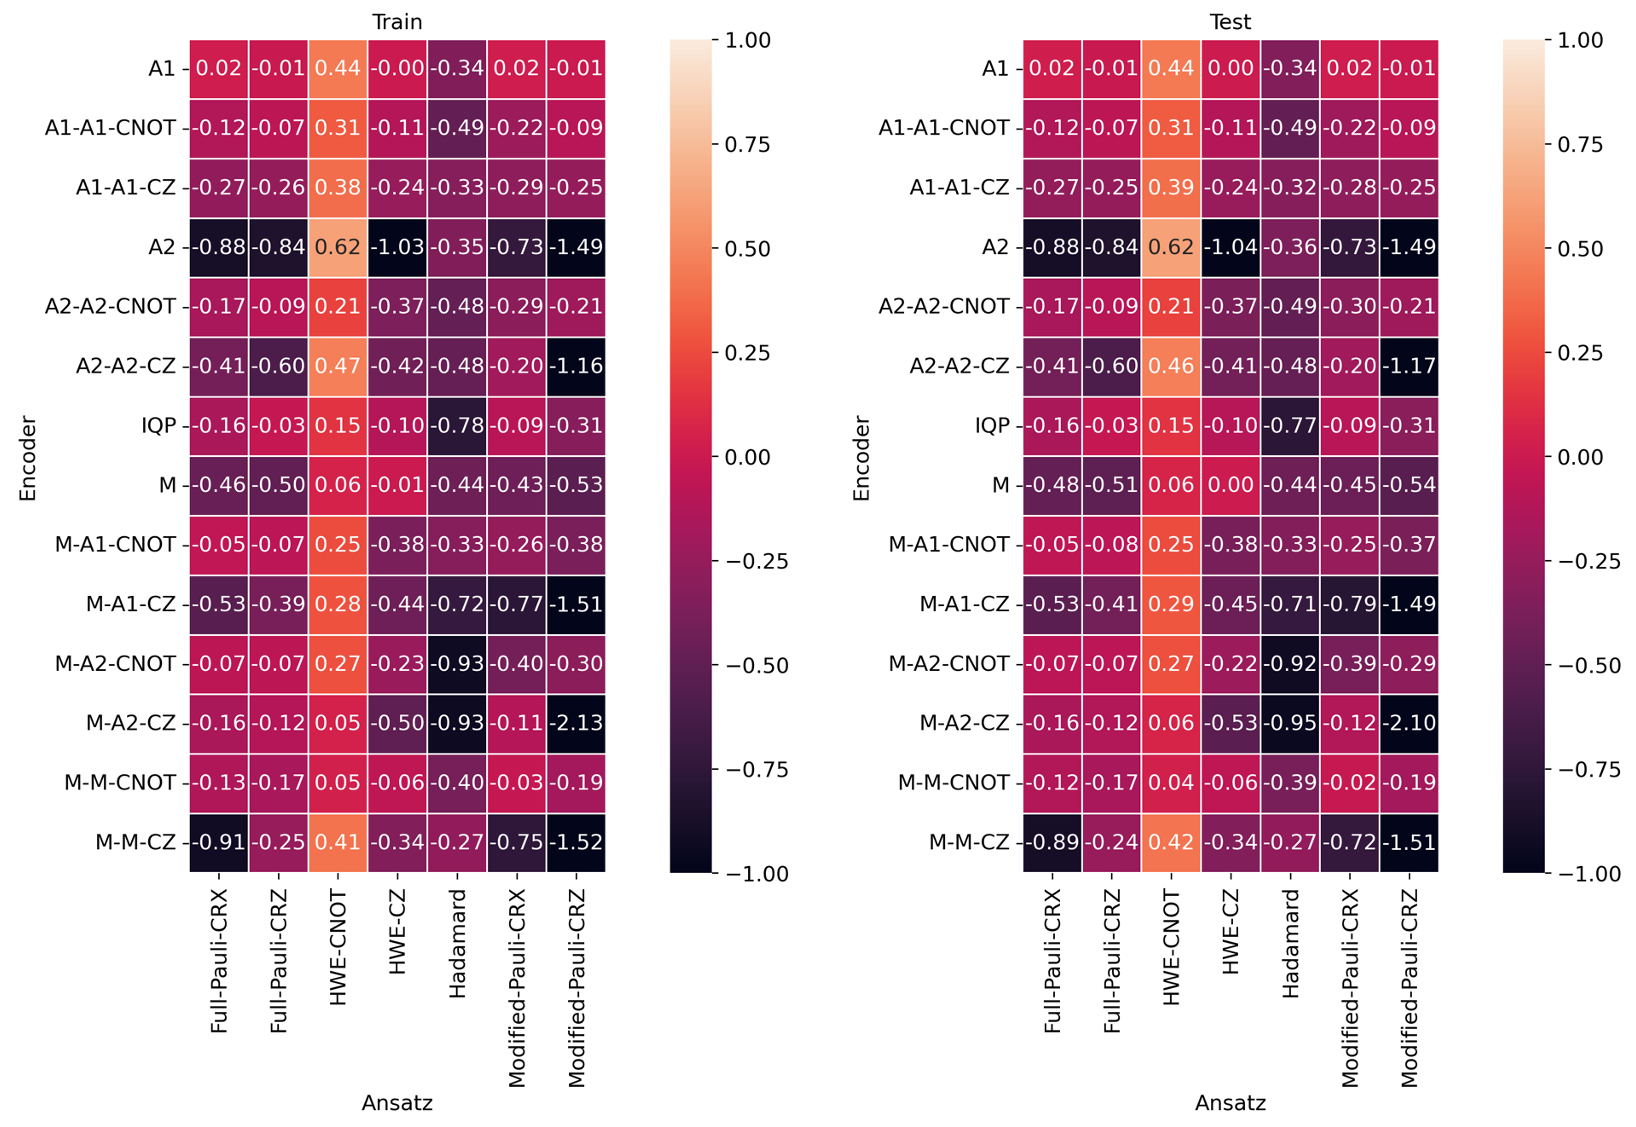
\includegraphics[width=\linewidth]{../images/DDCC/DDCC_heatplots}
		\caption{}
		\label{fig:ddccheatplots}
	\end{subfigure}
	\hfill	
	\begin{subfigure}[b]{0.49\textwidth}
		\centering
		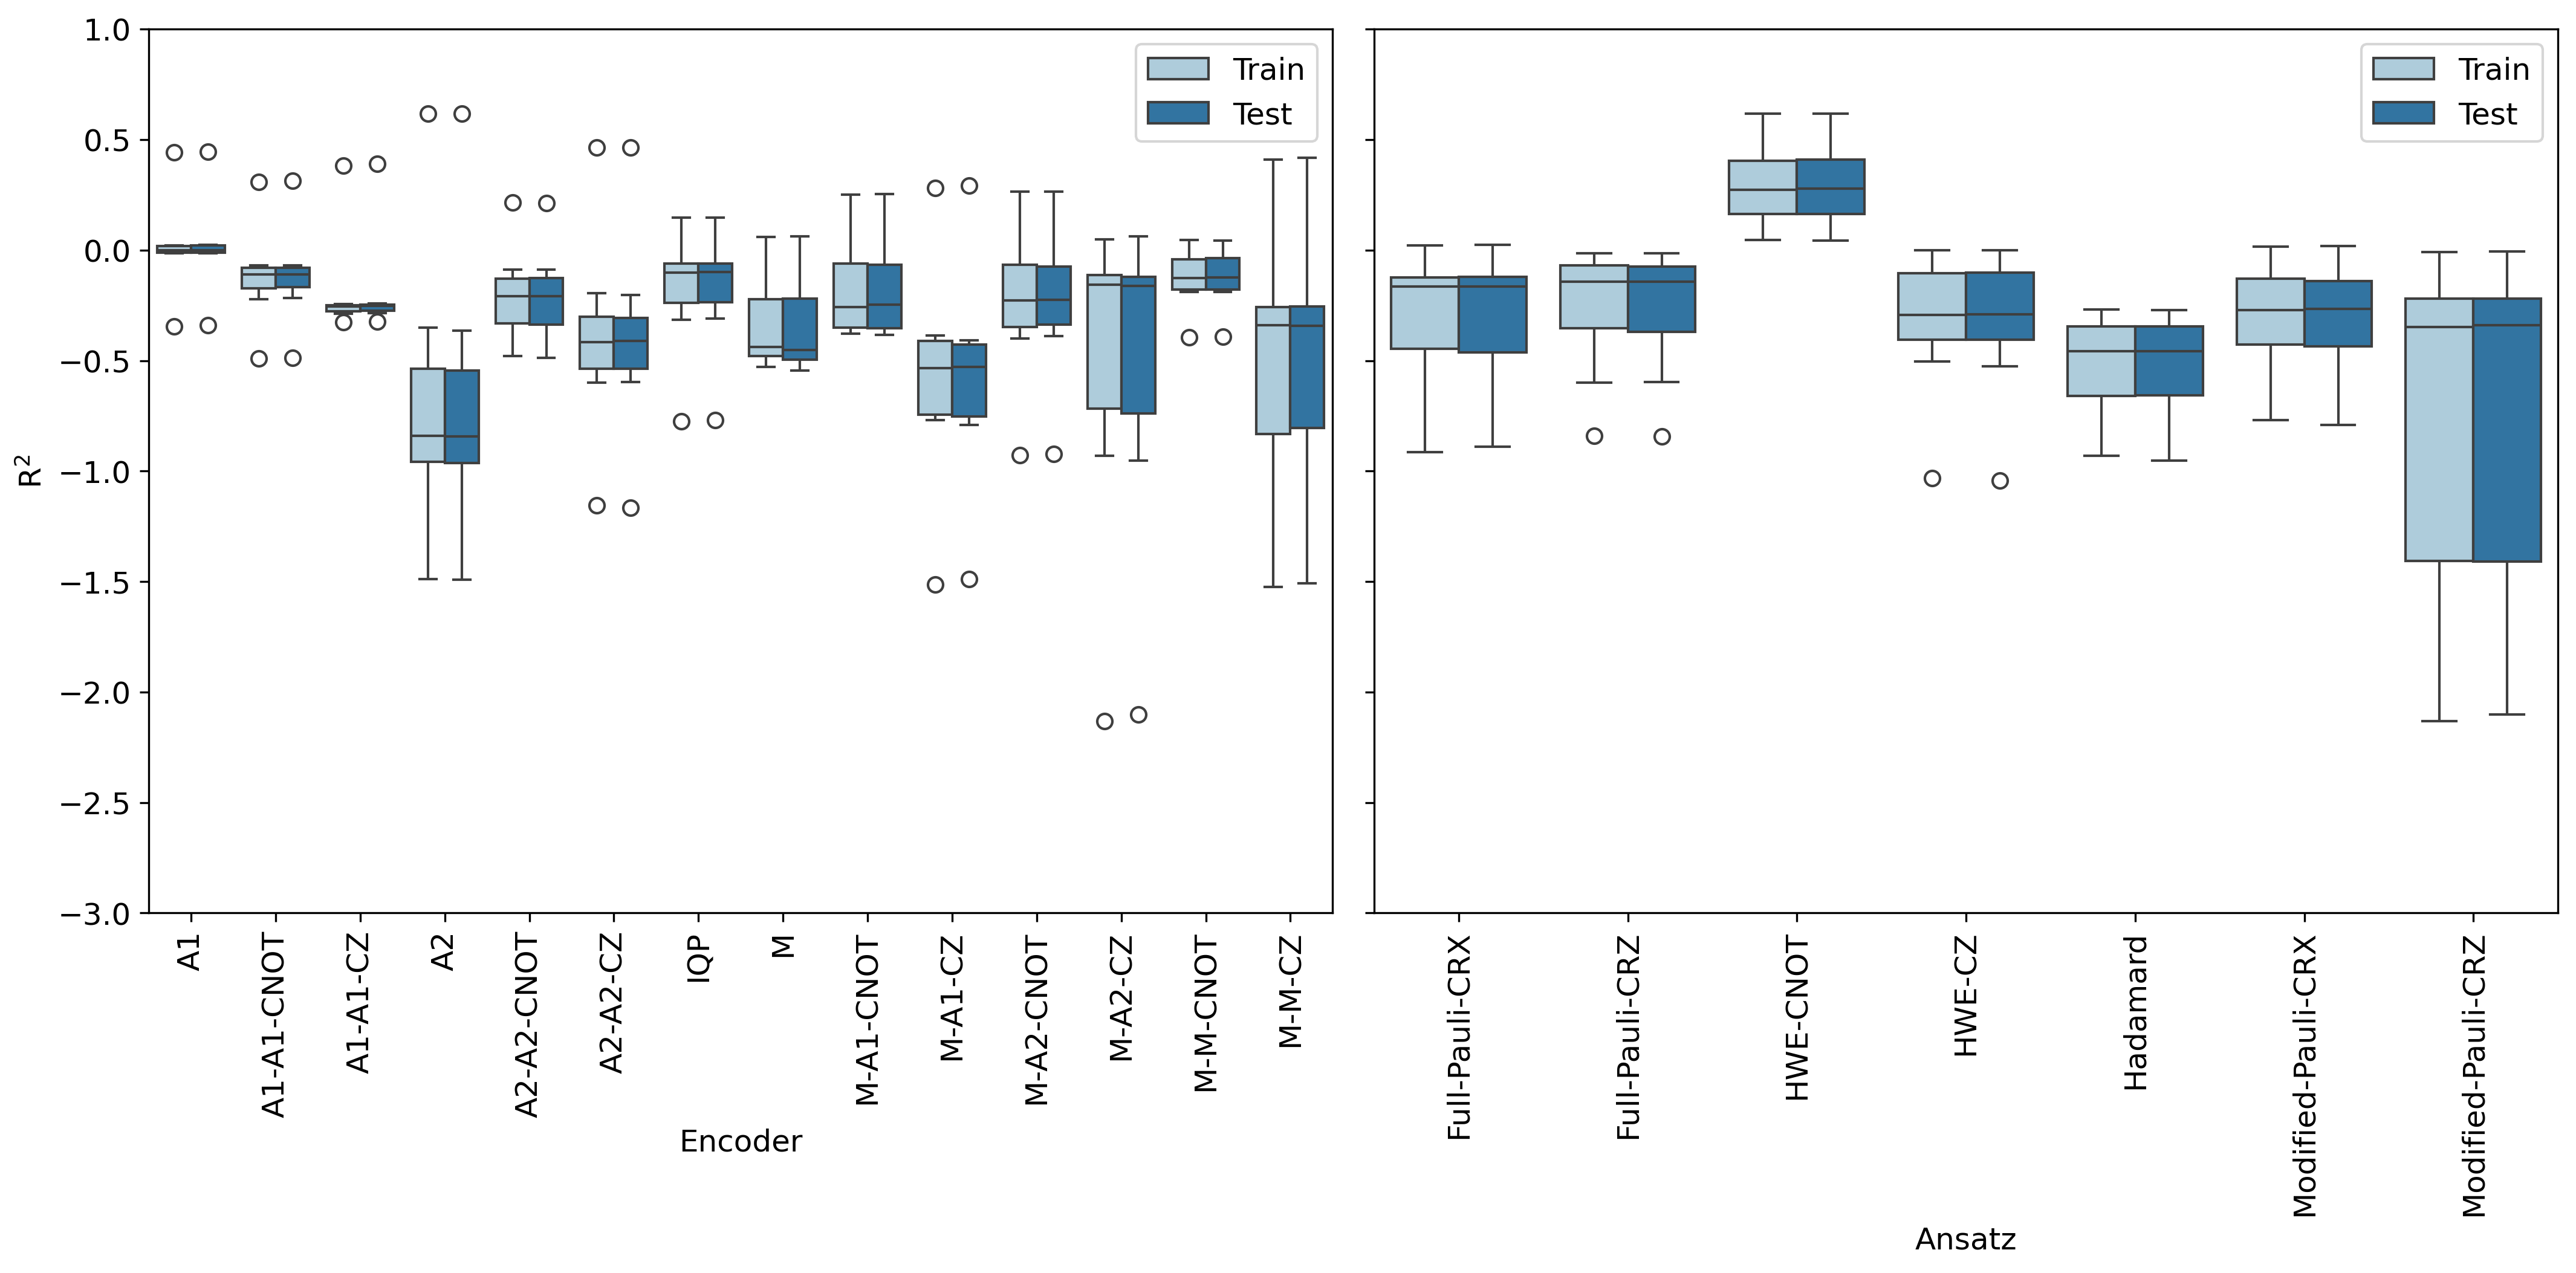
\includegraphics[width=\linewidth]{../images/DDCC/DDCC_boxplots}
		\caption{}
		\label{fig:ddccboxplots}
	\end{subfigure}
	\hfill
%	\begin{subfigure}[b]{0.49\textwidth}
%		\centering
%		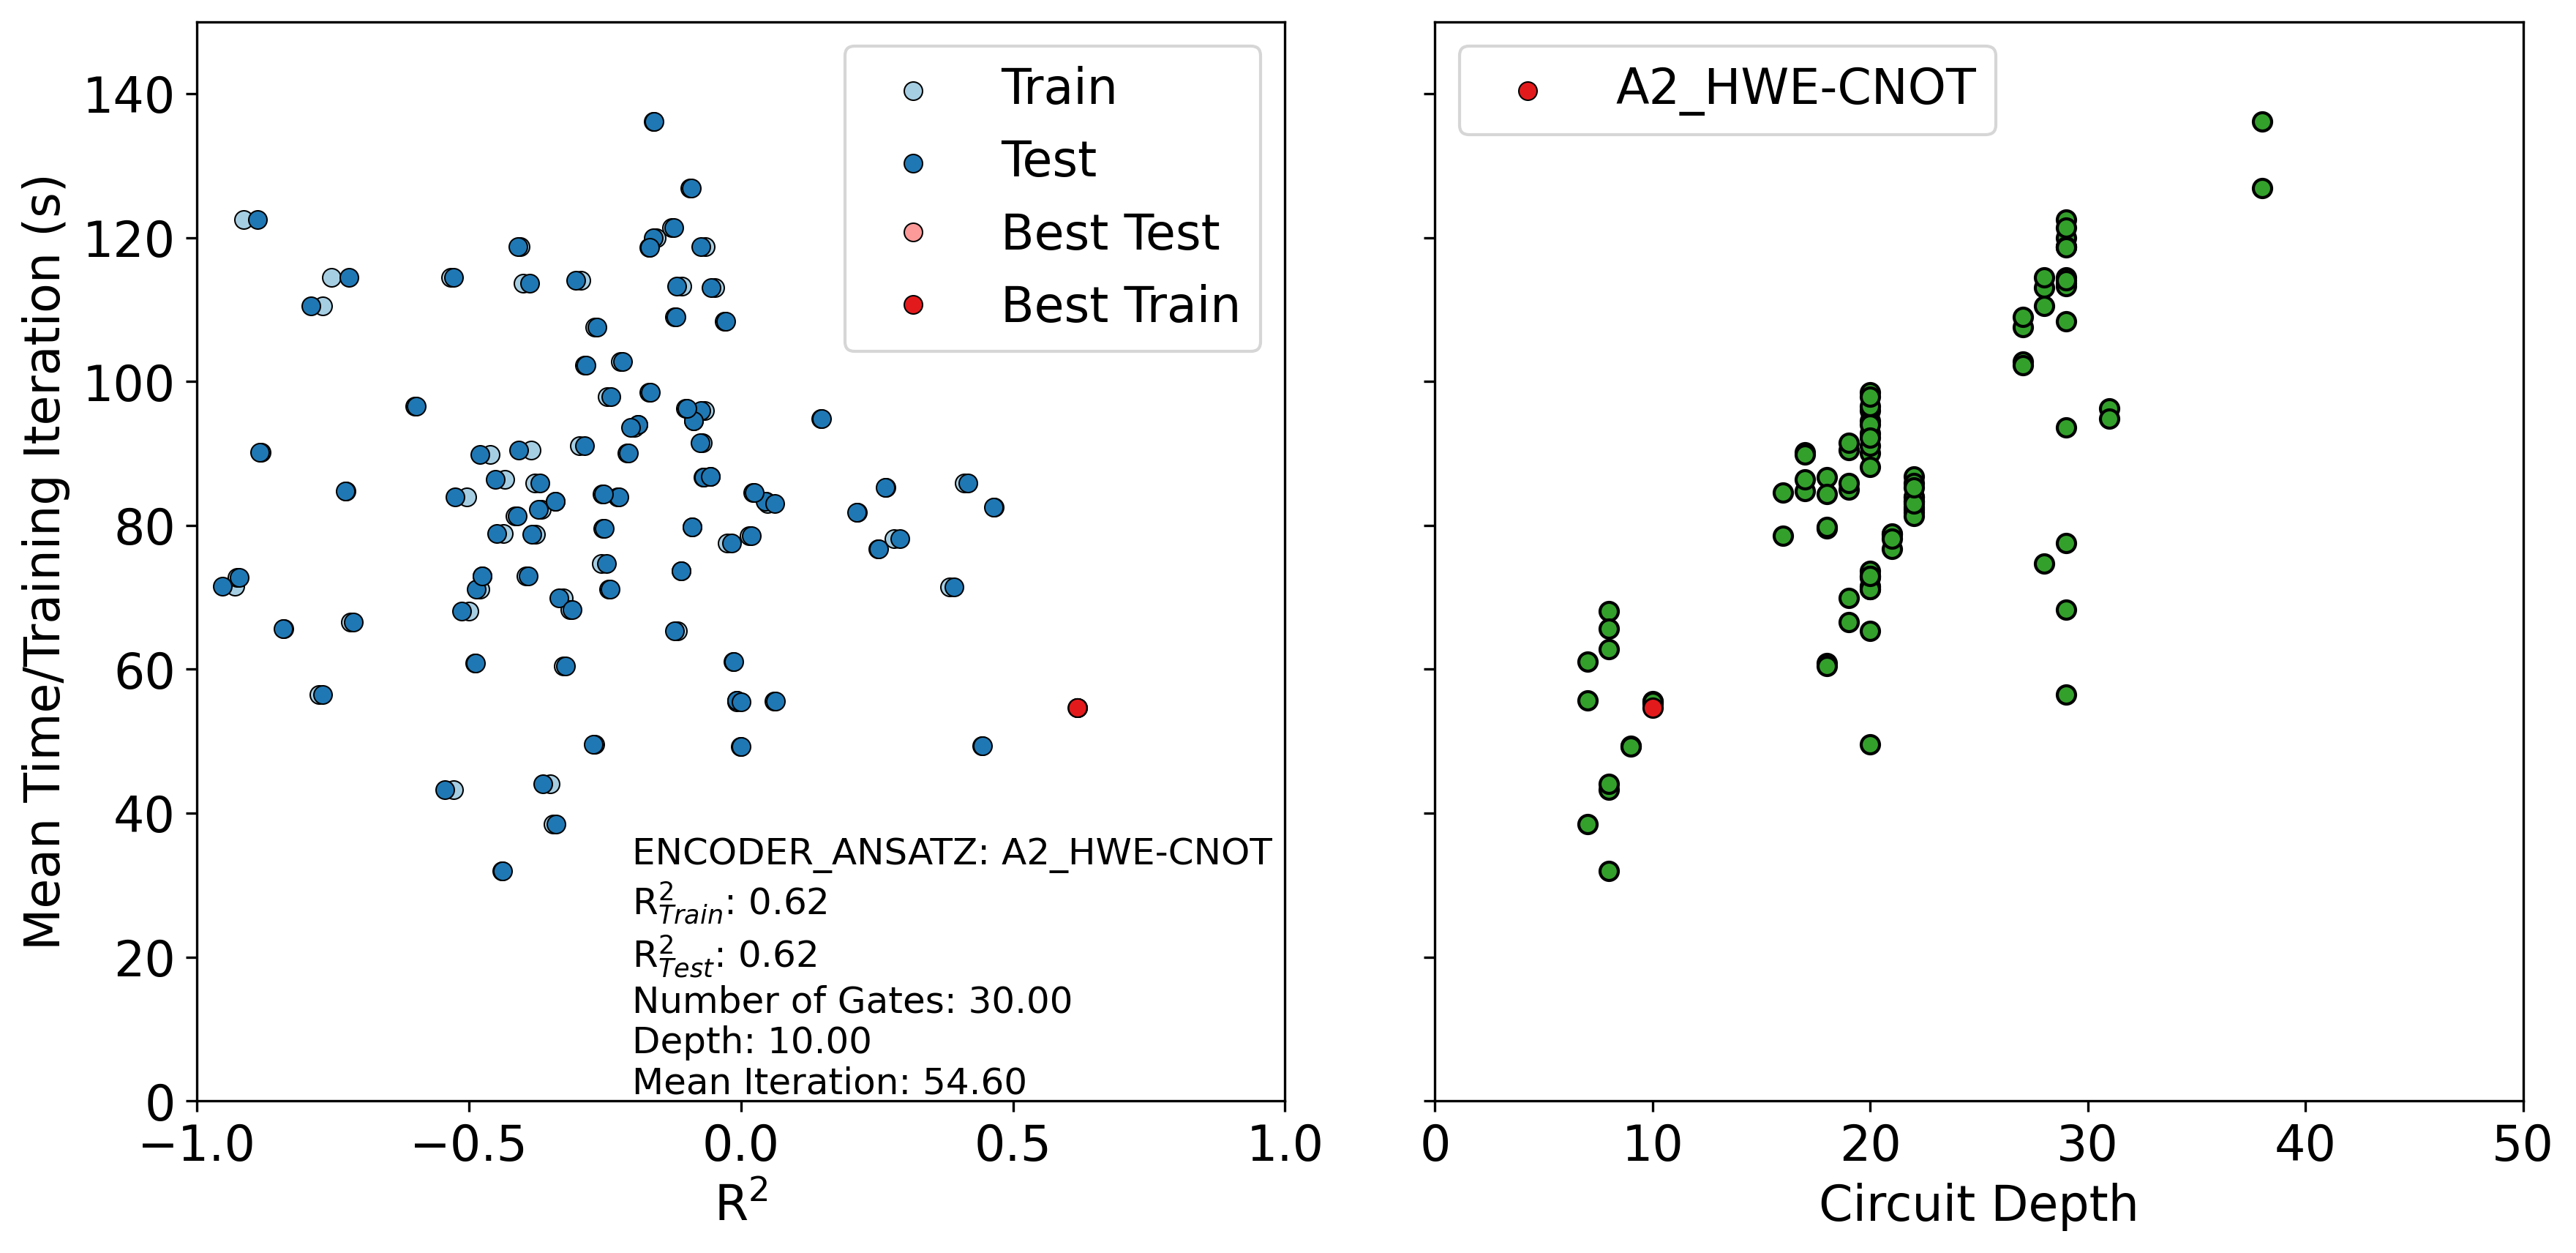
\includegraphics[width=\linewidth]{../images/DDCC/AllDDCC5_circuitdepth_R2_vs_iterationtime}
%		\caption{}
%		\label{fig:allddcc5circuitdepthr2vsiterationtime}
%	\end{subfigure}	
	\caption{}
	\label{fig:ddcc_all_analysis}	
\end{figure}


(AL,RUD)=(1,1) Train R$^{2}$ 0.62/test R$^{2}$ 0.62
(AL,RUD)=(1,3) Train R$^{2}$ 0.85/test R$^{2}$ 0.85
(AL,RUD)=(1,5) Train R$^{2}$ 0.82/test R$^{2}$ 0.83
(AL,RUD)=(3,1) Train R$^{2}$ 0.71/test R$^{2}$ 0.71
(AL,RUD)=(5,1) Train R$^{2}$ 0.77/test R$^{2}$ 0.77

Talk about the cost of going wider, and inherently deeper

\begin{figure}[H]
	\centering	
	\begin{subfigure}[b]{0.49\textwidth}
		\centering
		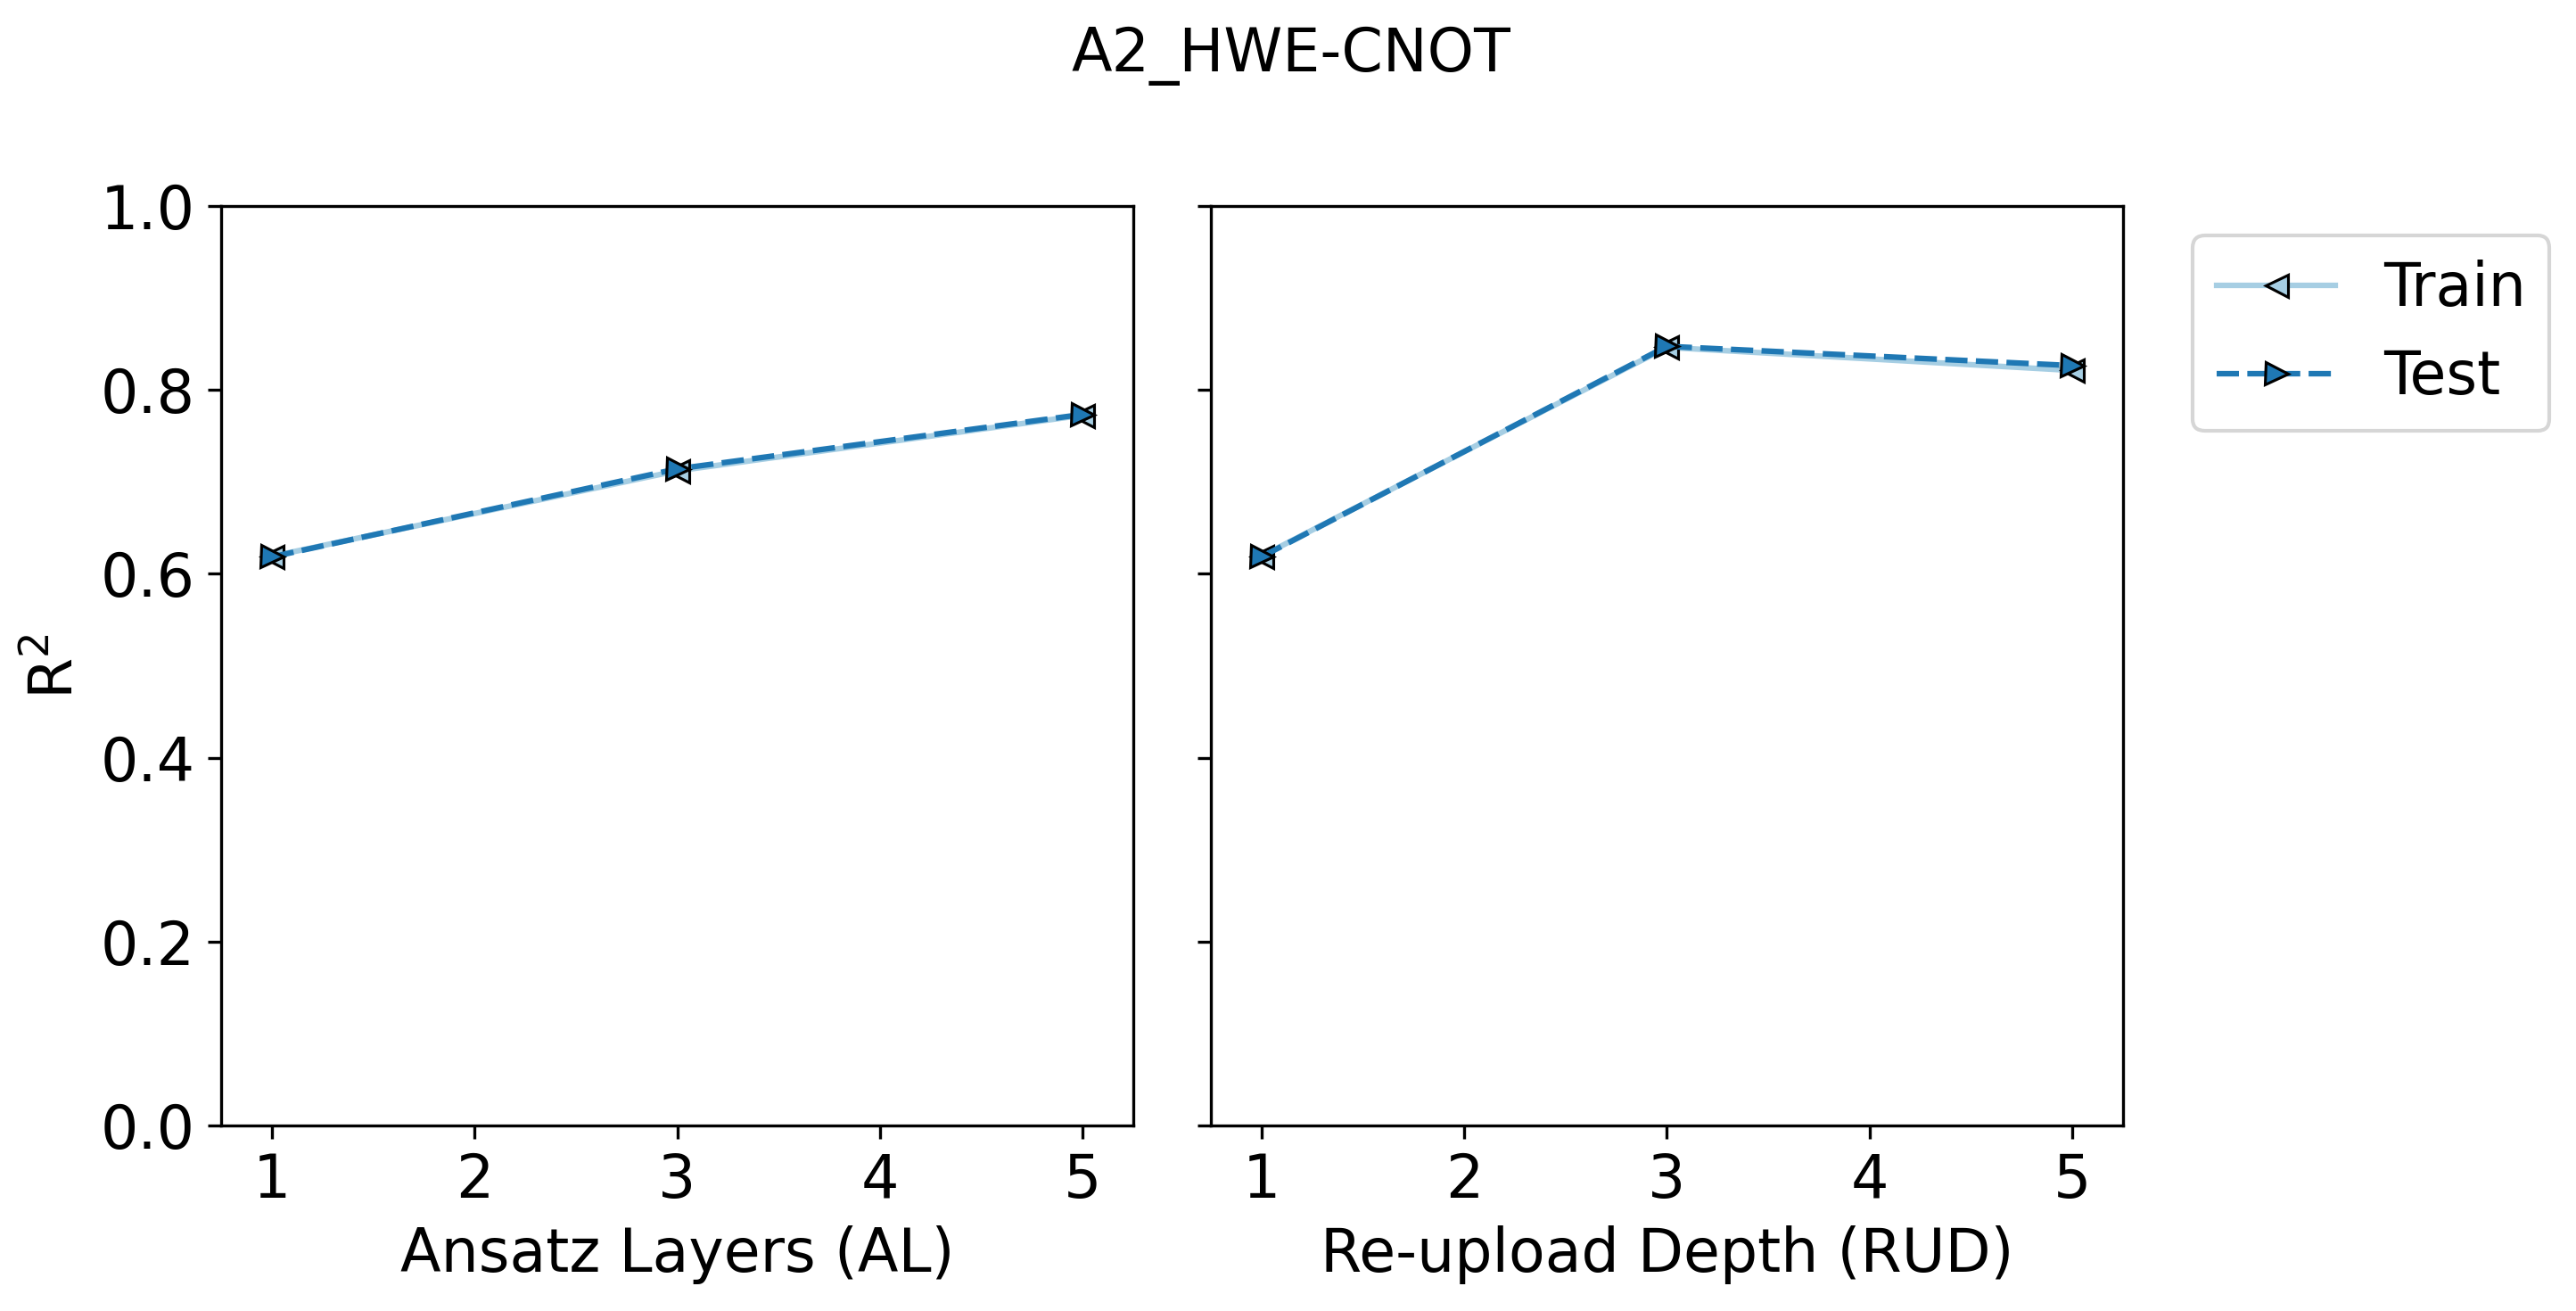
\includegraphics[width=\linewidth]{../images/DDCC/DDCC_RUDAL_lineplot}
		\caption{}
		\label{fig:ddccRUDAL_lineplot}
	\end{subfigure}
	\hfill
	\begin{subfigure}[b]{\textwidth}
		\centering
		\includegraphics[width=0.49\linewidth]{../images/DDCC/distribution_parity}
		\caption{}
		\label{fig:ddccdistribution_parity}
	\end{subfigure}
	\caption{Model evaluation, using R$^{2}$ (y-axis), of re-upload depths (RUD) and ansatz layers (AL) of 1, 3, and 5 for the A2\_HWE-CNOT using the DDCC dataset. The left side of the plot denotes the training set and the right side the test set.}
	\label{fig:ddcc_rud}	
\end{figure}




\begin{figure}[H]
	\centering
	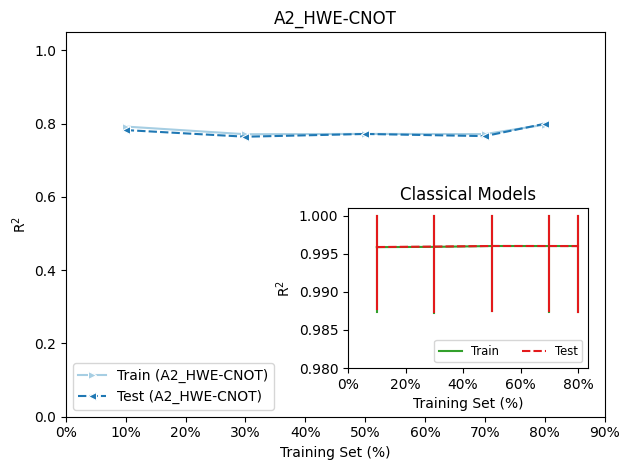
\includegraphics[width=\linewidth]{../images/DDCC/DDCC_learning_curves}
	\caption{}
	\label{fig:ddcclearningcurves}
\end{figure}

Ansaetze analysis \cite{sim_expressibility_2019}
``In particular, a substantial improvement in performance of two-qubit gates in a ring or all-to-all connected arrangement, compared to thatof those on a line, is observed.''

``Furthermore, improvement in both descriptors is achieved by sequences of controlled X-rotation gates compared tosequences of controlled Z-rotation gates.''

``investigated howexpressibility “saturates” with increased circuit depth, finding that the rateand saturated value appear to be distinguishing features of a PQC''



5 qubit/5 ansatz layers: 2*5 + 3 * 5 * 5 = 85 parameters (75 trainable, 5 * 2 features)
A2 $2n$ parameters
HWE-CNOT $3nL$ parameters
2 qubit gates $nL$
Number of parameters (2n+3nL)=(2+3L)*n

$n$, number of qubits and $L$, number of circuit layers

To efficiently run DDCC on IBM Quebec, splitting the data into batches of $\approx 4$ samples with 64 $t_{2}$-amplitudes each.

One iteration would require approximately $N_{\text{samples}} * N_{occ}^{2} * N_{virt}^{2} * N_{\text{shots}} * N_{\text{observables}}$ circuit executions (+ whatever SPSA costs to run per iteration)


Ran using the state vector model parameters for one iteration to test the optimization and resilience levels using Fake Quebec before running on the real device

$\{1024 \times x \vert  x \in [1,10]\}$ 

Fake
Optimization level 2 
resilience level 0

Regarding the number of circuit executions vs performance 3072 (1024 times 3) is the best number of shots


Fig. \ref{fig:optresfakequebec}
Fig. \ref{fig:shotsfakequebec}


Real
Optimization level 2 
resilience level 1
3072

resilience level 2 is too expensive on the real device
Regarding the number of circuit executions vs performance 3072 (1024 times 3) is the best number of shots


\section{Conclusion}
Quantum advantage in terms of computational complexity but not in model performance?


Depth is not always better!
Molecular representations specifically for QML
Distributed QC to incorporate more features
Noiseless simulation is costly and does not offer the desired accuracy for BSE49 or DDCC

DDCC could be a useful dataset to benchmark PQC models since it is trivial to perform classically, yet hard for PQCs...

\bibliography{achemso-demo}

\end{document}
